\section{Window Calculation Module}\label{window-calculation-module}

This section describes two potential modeling approaches for Windows.~ The first (layer by layer) is implemented.~ The second, simple approach, reuses the layer-by-layer approach but converts an arbitrary window performance into an equivalent single layer.

The primary Window calculation is a layer-by-layer approach where windows are considered to be composed of the following components, only the first of which, glazing, is required to be present:

\begin{itemize}
\item
  \textbf{\emph{Glazing}}, which consists of one or more plane/parallel glass layers. If there are two or more glass layers, the layers are separated by gaps filled with air or another gas. The glazing optical and thermal calculations are based on algorithms from the WINDOW 4 and WINDOW 5 programs {[}Arasteh et al., 1989{]}, {[}Finlayson et al., 1993{]}.~ Glazing layers are described using te input object WindowMaterial:Glazing.
\item
  \textbf{\emph{Gap}}, layers filled with air or another gas that separate glazing layers.~ Gaps are described using the input object WindowMaterial:Gas.
\item
  \textbf{\emph{Frame}}, which surrounds the glazing on four sides.~ Frames are described using the input object WindowProperty:FrameAndDivider.
\item
  \textbf{\emph{Divider}}, which consists of horizontal and/or vertical elements that divide the glazing into individual lites.
\item
  \textbf{\emph{Shading device}}, which is a separate layer, such as drapery, roller shade or blind, on the inside or outside of the glazing, whose purpose is to reduce solar gain, reduce heat loss (movable insulation) or control daylight glare.~ Shading layers are described using ``WindowProperty:ShadingControl'' input objects.
\end{itemize}

In the following, the description of the layer-by-layer glazing algorithms is based on material from Finlayson et al., 1993. The frame and divider thermal model, and the shading device optical and thermal models, are new to EnergyPlus.

A second approch has been developed where windows are modeled in a simplified approach that requires minimal user input that is processed to develop and equivalent layer that then reuses much of the layer-by-model.~ This ``Simple Window Construction: model is described below.

\subsection{Optical Properties of Glazing}\label{optical-properties-of-glazing}

The solar radiation transmitted by a system of glass layers and the solar radiation absorbed in each layer depends on the solar transmittance, reflectance and absorptance properties of the individual layers. The absorbed solar radiation enters the glazing heat balance calculation that determines the inside surface temperature and, therefore, the heat gain to the zone from the glazing (see ``Window Heat Balance Calculation''). The transmitted solar radiation is absorbed by interior zone surfaces and, therefore, contributes to the zone heat balance. In addition, the visible transmittance of the glazing is an important factor in the calculation of interior daylight illuminance from the glazing.

% table 28
\begin{longtable}[c]{p{1.0in}p{2.5in}p{1.0in}p{1.5in}}
\caption{Variables in Window Calculations \label{table:variables-in-window-calculations}} \tabularnewline
\toprule 
Mathematical variable & Description & Units & FORTRAN variable \tabularnewline
\midrule
\endfirsthead

\caption[]{Variables in Window Calculations} \tabularnewline
\toprule 
Mathematical variable & Description & Units & FORTRAN variable \tabularnewline
\midrule
\endhead

T & Transmittance & - & - \tabularnewline
R & Reflectance & - & - \tabularnewline
R\(^{f}\), R\(^{b}\) & Front reflectance, back reflectance & - & - \tabularnewline
T\(_{i,j}\) & Transmittance through glass layers i to j & - & - \tabularnewline
T\(^{dir}_{gl}\) & Direct transmittance of glazing & - & - \tabularnewline
R\(^{f}_{i,j}\), R\(^{b}_{i,j}\) & Front reflectance, back reflectance from glass layers i to j & - & - \tabularnewline
R\(^{dir}_{gl,f}\), R\(^{dir}_{gl,b}\) & Direct front and back reflectance of glazing & - & - \tabularnewline
A\(^{f}_{i}\), A\(^{b}_{i}\) & Front~ absorptance, back absorptance of layer i & - & - \tabularnewline
N & Number of glass layers & - & Nlayer \tabularnewline
$\lambda$ & Wavelength & microns & Wle \tabularnewline
E\(_{s}\) ($\lambda$) & Solar spectral irradiance function & W/m\(^{2}\)-micron & E \tabularnewline
V($\lambda$) & Photopic response function of the eye & - & y30 \tabularnewline
$\varphi$ & Angle of incidence (angle between surface normal and direction of incident beam radiation) & Rad & Phi \tabularnewline
$\tau$ & Transmittivity or transmittance & - & tf0 \tabularnewline
$\rho$ & Reflectivity or reflectance & - & rf0, rb0 \tabularnewline
$\alpha$ & Spectral absorption coefficient & m\(^{-1}\) & - \tabularnewline
d & Glass thickness & M & Material\%Thickness \tabularnewline
n & Index of refraction & - & ngf, ngb \tabularnewline
$\kappa$ & Extinction coefficient & - & - \tabularnewline
$\beta$ & Intermediate variable & - & betaf, betab \tabularnewline
P, p & A general property, such as transmittance & - & - \tabularnewline
$\tau$\(_{sh}\) & Shade transmittance & - & Material\%Trans \tabularnewline
$\rho$\(_{sh}\) & Shade reflectance & - & Material\%ReflectShade \tabularnewline
$\alpha$\(_{sh}\) & Shade absorptance & - & Material\%AbsorpSolar \tabularnewline
$\tau$\(_{bl}\) $\rho$\(_{bl}\) $\alpha$\(_{bl}\) & Blind transmittance, reflectance, absorptance & - & - \tabularnewline
Q, G, J & Source, irradiance and radiosity for blind optical properties calculation & W/m\(^{2}\) & - \tabularnewline
F\(_{ij}\) & View factor between segments i and j & - & - \tabularnewline
f\(_{switch}\) & Switching factor & - & SwitchFac \tabularnewline
T & Transmittance & - & - \tabularnewline
R & Reflectance & - & - \tabularnewline
R\(^f\), R\(^b\) & Front reflectance, back reflectance & - & - \tabularnewline
T\(_{i,j}\) & Transmittance through glass layers i to j & - & - \tabularnewline
R\(^f_{i,j}\), R\(^b_{i,j}\) & Front reflectance, back reflectance from glass layers i to j & - & - \tabularnewline
A\(^f_i\), A\(^b_i\) & Front~ absorptance, back absorptance of layer i & - & - \tabularnewline
N & Number of glass layers & - & Nlayer \tabularnewline
\(\lambda\) & Wavelength & microns & Wle \tabularnewline
E\(_s (\lambda)\) & Solar spectral irradiance function & W/m\(^2\)-micron & E \tabularnewline
R($\lambda$) & Photopic response function of the eye & - & y30 \tabularnewline
$\varphi$' & Relative azimuth angle (angle between screen surface normal and vertical plane through sun, Ref. Figure 87) & Rad & SunAzimuthToScreenNormal \tabularnewline
$\alpha$' & Relative altitude angle (angle between screen surface horizontal normal plane and direction of incident beam radiation, Ref. Figure 87) & Rad & SunAltitudeToScreenNormal \tabularnewline
$\rho$\(_{sc}\) & Beam-to-diffuse solar reflectance of screen material & - & Screens\%ReflectCylinder \tabularnewline
$\gamma$ & Screen material aspect ratio & - & Screens\%ScreenDiameterTo SpacingRatio \tabularnewline
Α & Spectral absorption coefficient & m\(^{-1}\) & - \tabularnewline
D & Glass thickness & M & Material\%Thickness \tabularnewline
N & Index of refraction & - & ngf, ngb \tabularnewline
Κ & Extinction coefficient & - & - \tabularnewline
Β & Intermediate variable & - & betaf, betab \tabularnewline
P, p & A general property, such as transmittance & - & - \tabularnewline
\bottomrule
\end{longtable}

\subsection{Glass Layer Properties}\label{glass-layer-properties}

In EnergyPlus, the optical properties of individual glass layers are given by the following quantities at normal incidence as a function of wavelength:

Transmittance, \emph{T}

Front reflectance, \emph{R\(^{f}\)}

Back reflectance, \emph{R\(^{b}\)}

Here ``front'' refers to radiation incident on the side of the glass closest to the outside environment, and ``back'' refers to radiant incident on the side of the glass closest to the inside environment. For glazing in exterior walls, ``front'' is therefore the side closest to the outside air and ``back'' is the side closest to the zone air. For glazing in interior (i.e., interzone) walls, ``back'' is the side closest to the zone in which the wall is defined in and ``front'' is the side closest to the adjacent zone.

\subsection{Glass Optical Properties Conversion}\label{glass-optical-properties-conversion}

\subsubsection{Conversion from Glass Optical Properties Specified as Index of Refraction and Transmittance at Normal Incidence}\label{conversion-from-glass-optical-properties-specified-as-index-of-refraction-and-transmittance-at-normal-incidence}

The optical properties of uncoated glass are sometimes specified by index of refraction, \emph{n},* * and transmittance at normal incidence, \emph{T}.

The following equations show how to convert from this set of values to the transmittance and reflectance values required by Material:WindowGlass. These equations apply only to uncoated glass, and can be used to convert either spectral-average solar properties or spectral-average visible properties (in general, \emph{n} and \emph{T} are different for the solar and visible). Note that since the glass is uncoated, the front and back reflectances are the same and equal to the \emph{R} that is solved for in the following equations.

Given \emph{n} and \emph{T}, find \emph{R}:

\begin{equation}
  \begin{array}{l}
    r = \left( \frac{n - 1}{n + 1} \right)^2 \\
    \tau  = \frac{\left[ (1 - r)^4 + 4 r^2 T^2 \right]^{1/2} - (1 - r)^2}{2 r^2 T} \\
    R = r + \frac{(1 - r)^2 r \tau ^2}{1 - r^2 \tau ^2}
  \end{array}
\end{equation}

\textbf{Example:}

\emph{T} = 0.86156

\emph{n} = 1.526

\begin{equation}
  \begin{array}{l}
    r = \left( \frac{1.526 - 1}{1.526 + 1} \right)^2 \\
    \tau = 0.93974 \\
    R = 0.07846
  \end{array}
\end{equation}

\subsection{Simple Window Model}\label{simple-window-model}

EnergyPlus includes an alternate model that allows users to enter in simplified window performance indices.~ This model is accessed through the WindowMaterial:SimpleGlazingSystem input object and converts the simple indices into an equivalent single layer window.~ (In addition a special model is used to determine the angular properties of the system -- described below).~ Once the model generates the properties for the layer, the program reuses the bulk of the layer-by-layer model for subsequent calculations.~ The properties of the equivalent layer are determined using the step by step method outlined by Arasteh, Kohler, and Griffith (2009).~ The core equations are documented here.~ The reference contains additional information.

The simplified window model accepts U and SHGC indices and is useful for several reasons:

1)~~~Sometimes, the only thing that is known about the window are its U and SHGC;

2)~~~Codes, standards, and voluntary programs are developed in these terms;

3)~~~A single-layer calculation is faster than multi-layer calculations.

Note: This use of U and SHGC to describe the thermal properties of windows is only appropriate for specular glazings.

While it is important to include the ability to model windows with only U-value and SHGC, we note that any method to use U and SHGC alone in building simulation software will inherently be approximate.~ This is due primarily to the following factors:

\begin{itemize}
\item
  SHGC combines directly transmitted solar radiation and radiation absorbed by the glass which flows inward.~ These have different implications for space heating/cooling.~ Different windows with the same SHGC often have different ratios of transmitted to absorbed solar radiation.
\item
  SHGC is determined at normal incidence; angular properties of glazings vary with number of layers, tints, coatings.~ So products which have the same SHGC, can have different angular properties.
\item
  Window U-factors vary with temperatures.
\end{itemize}

Thus, for modeling specific windows, we recommend using more detailed data than just the U and SHGC, if at all possible.

The simplified window model determines the properties of an equivalent layer in the following steps.

\subsubsection{Step 1.~ Determine glass-to-glass Resistance.}\label{step-1.-determine-glass-to-glass-resistance.}

Window U-values include interior and exterior surface heat transfer coefficients.~ The resistance of the bare window product, or glass-to-glass resistance is augmented by these film coefficients so that,

\begin{equation}
\frac{1}{U} = {R_{i,w}} + {R_{o,w}} + {R_{l,w}}
\end{equation}

Where,

\({R_{i,w}}\) ~is the resistance of the interior film coefficient under standard winter conditions in units of m\(^{2}\)·K/W,

\({R_{o,w}}\) ~is the resistance of the exterior film coefficient under standard winter conditions in units of m\(^{2}\)·K/W, and

\({R_{l,w}}\) ~is the resisance of the bare window under winter conditions (without the film coefficients) in units of m\(^{2}\)·K/W.

The values for \({R_{i,w}}\) ~and \({R_{o,w}}\) ~depend on U and are calculated using the following correlations.

\begin{equation}
{R_{i,w}} = \frac{1}{{(0.359073\;Ln(U) + 6.949915)}};\quad for\quad U < 5.85
\end{equation}

\begin{equation}
{R_{i,w}} = \frac{1}{{(1.788041\;U - 2.886625)}};\quad for\quad U \ge 5.85
\end{equation}

\begin{equation}
{R_{o,w}} = \frac{1}{{(0.025342\;U + 29.163853)}}
\end{equation}

So that the glass-to-glass resistance is calculated using,

\({R_{l,w}} = \frac{1}{U} - {R_{i,w}} - {R_{o,w}}\) .

Because the window model in EnergyPlus is for flat geometries, the models are not necessarily applicable to low-performance projecting products, such as skylights with unisulated curbs.~ The model cannot support glazing systems with a U higher than 7.0 because the thermal resistance of the film coefficients alone can provide this level of performance and none of the various resistances can be negative.

\subsubsection{Step 2.~ Determine Layer Thickness.}\label{step-2.-determine-layer-thickness.}

The thickness of the equivalent layer in units of meters is calculated using,

\begin{equation}
  Thickness = \left\{
                \begin{array}{cl}
                  0.002                             & for \frac{1}{R_{l,w}} > 7.0 \\
                  0.05914 - \frac{0.00714}{R_{l,w}} & for \frac{1}{R_{l,w}} \leq 7.0
                \end{array}
              \right.
\end{equation}

\subsubsection{Step 3.~ Determine Layer Thermal Conductivity}\label{step-3.-determine-layer-thermal-conductivity}

The effective thermal conductivity, \({\lambda_{eff}}\) , of the equivalent layer is calculated using,

\begin{equation}
{\lambda_{eff}} = \frac{{Thickness}}{{{R_{l,w}}}}
\end{equation}

\subsubsection{Step 4.~ Determine Layer Solar Transmittance}\label{step-4.-determine-layer-solar-transmittance}

The layer's solar transmittance at normal incidence, \({T_{sol}}\) , is calculated using correlations that are a function of SHGC and U-Factor.

\begin{equation}
{T_{sol}} = 0.939998\;SHG{C^2} + 0.20332\;SHGC;\quad U > 4.5;\;SHGC < 0.7206
\end{equation}

\begin{equation}
{T_{sol}} = 1.30415SHGC - 0.30515\;;\quad U > 4.5;\;SHGC \ge 0.7206
\end{equation}

\begin{equation}
{T_{sol}} = 0.41040\;SHGC;\quad U < 3.4;\;SHGC \le 0.15
\end{equation}

\begin{equation}
{T_{sol}} = 0.085775\;SHG{C^2} + 0.963954\;SHGC - 0.084958\;;\;\;U < 3.4;\;SHGC > 0.15
\end{equation}

And for U-values between 3.4 and 4.5, the value for \({T_{sol}}\) ~is interpolated using results of the equations for both ranges.

\subsubsection{Step 5.~ Determine Layer Solar Reflectance}\label{step-5.-determine-layer-solar-reflectance}

The layer's solar reflectance is calculated by first determining the inward flowing fraction which requires values for the resistance of the inside and outside film coefficients under summer conditions, \({R_{i,s}}\) ~and \({R_{o,s}}\) respectively.~ The correlations are

{\scriptsize
\begin{equation}
\begin{split}
&{R_{i,s}} = \frac{1}{{\left( {29.436546\;{{\left( {SHGC - {T_{Sol}}} \right)}^3} - 21.943415{{\left( {SHGC - {T_{Sol}}} \right)}^2} + 9.945872\left( {SHGC - {T_{Sol}}} \right) + 7.426151} \right)}}; U > 4.5 \\
&{R_{i,s}} = \frac{1}{{\left( {199.8208128\;{{\left( {SHGC - {T_{Sol}}} \right)}^3} - 90.639733{{\left( {SHGC - {T_{Sol}}} \right)}^2} + 19.737055\left( {SHGC - {T_{Sol}}} \right) + 6.766575} \right)}}; U < 3.4 \\
&{R_{o,s}} = \frac{1}{{\left( {2.225824(SHGC - {T_{Sol}}) + 20.57708} \right)}}; U > 4.5 \\
&{R_{o,s}} = \frac{1}{{\left( {5.763355(SHGC - {T_{Sol}}) + 20.541528} \right)}}; U < 3.4
\end{split}
\end{equation}}

And for U-values between 3.4 and 4.5, the values are interpolated using results from both sets of equations.

The inward flowing fraction, \(Fra{c_{inward}}\) , is then calculated using

\begin{equation}
Fra{c_{inward}} = \frac{{\left( {{R_{o,s}} + 0.5\,{R_{l,w}}} \right)}}{{\left( {{R_{o,s}} + {R_{l,w}} + {R_{i,s}}} \right)}}
\end{equation}

The the solar reflectances of the front face, \({R_{s,f}}\) , and back face, \({R_{s,b}}\) , are calculated using,

\({R_{s,f}} = {R_{s,b}} = 1 - {T_{Sol}} - \frac{{\left( {SHGC - {T_{Sol}}} \right)}}{{Fra{c_{inward}}}}\) .

The thermal absorptance, or emittance, is take as 0.84 for both the front and back and the longwave transmittance is 0.0.

\subsubsection{Step 6.~ Determine Layer Visible Properties}\label{step-6.-determine-layer-visible-properties}

The user has the option of entering a value for visible transmittance as one of the simple performance indices.~ If the user does not enter a value, then the visible properties are the same as the solar properties.~ If the user does enter a value then layer's visible transmittance at normal incidence, \({T_{Vis}}\) ,is set to that value.~ The visible light reflectance for the back surface is calculated using,

\begin{equation}
{R_{Vis,b}} =  - 0.7409\,T_{Vis}^3 + 1.6531\,T_{Vis}^2 - 1.2299\,{T_{Vis}} + 0.4547
\end{equation}

The visible light reflectance for the front surface is calculated using,

\begin{equation}
{R_{Vis,f}} =  - 0.0622\,T_{Vis}^3 + 0.4277\,T_{Vis}^2 - 0.4169\,{T_{Vis}} + 0.2399
\end{equation}

\subsubsection{Step 7. Determine Angular Performance}\label{step-7.-determine-angular-performance}

The angular properties of windows are important because during energy modeling, the solar incidence angles are usually fairly high.~ Angles of incidence are defined as angles from the normal direction extending out from the window.~ The simple glazing system model includes a range of correlations that are selected based on the values for U and SHGC.~ These were chosen to match the types of windows likely to have such performance levels.~ The matrix of possible combinations of U and SHGC values have been mapped to set of 28 bins shown in the following figure.

\begin{figure}[hbtp] % fig 74
\centering
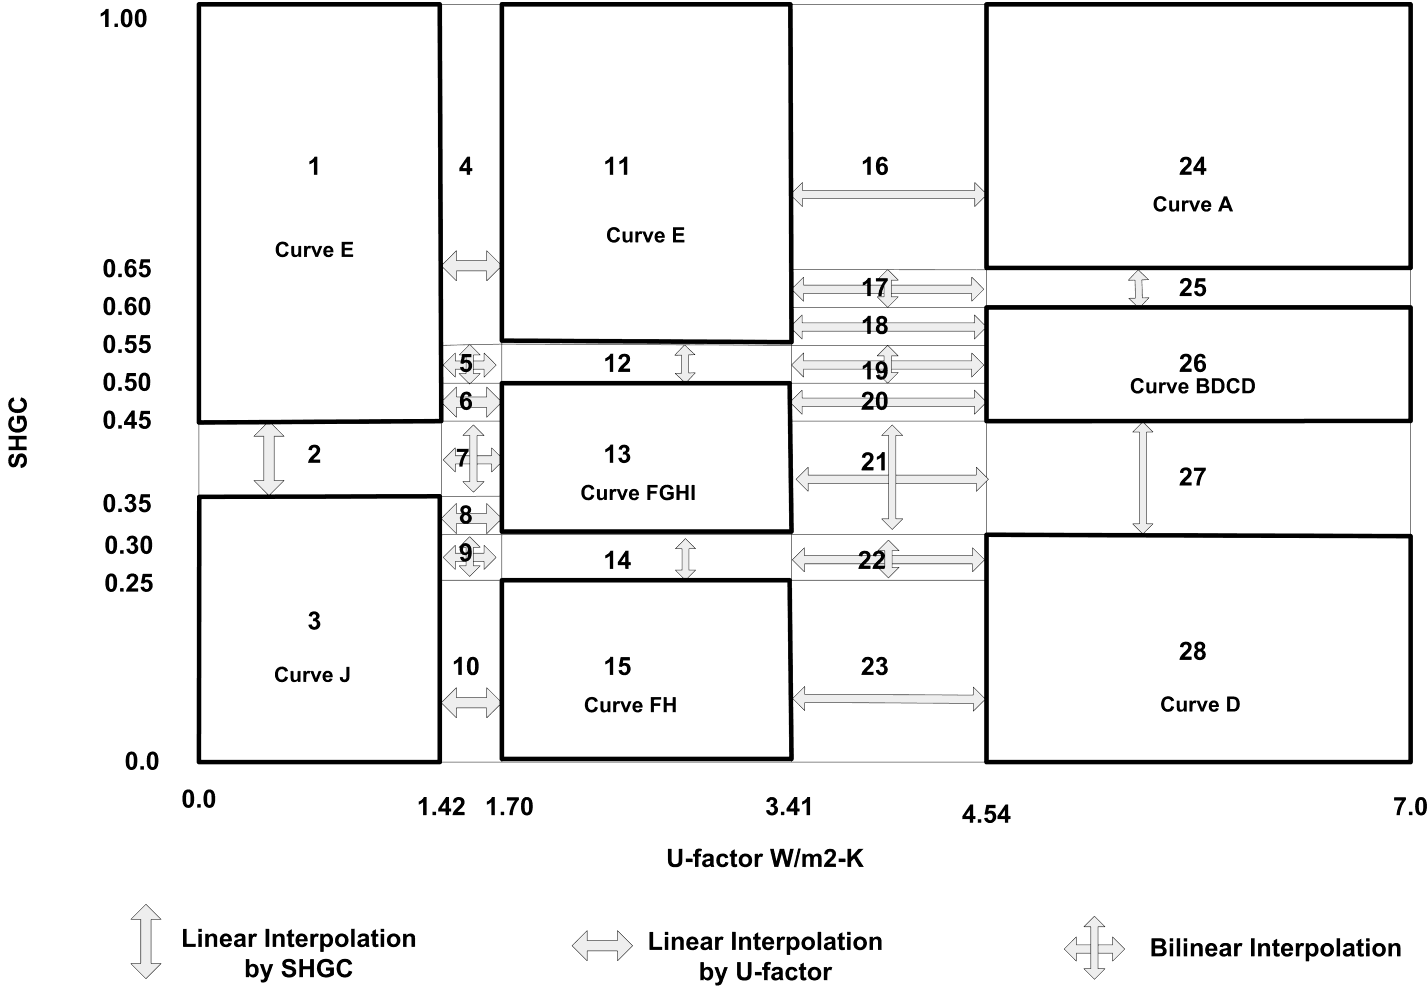
\includegraphics[width=0.9\textwidth, height=0.9\textheight, keepaspectratio=true]{media/image947.png}
\caption{Diagram of Transmittance and Reflectance Correlations Used based on U and SHGC \label{fig:diagram-of-transmittance-and}}
\end{figure}

There are ten different correlations, A thru J, for both transmission and reflectance.~ The correlations are used in various weighting and interpolation schemes according the figure above.~ The correlations are normalized against the performance at normal incidence.~ EnergyPlus uses these correlations to store the glazing system's angular performance at 10 degree increments and interpolates between them during simulations.~ The model equations use the cosine of the incidence angle, \(\cos (\varphi )\) , as the independent variable.~ The correlations have the form:

\begin{equation}
T\;or\;R = a\cos {(\varphi )^4} + b\cos {(\varphi )^3} + c\cos {(\varphi )^2} + d\cos (\varphi ) + e
\end{equation}

The coefficient values for a, b, c, d, and e are listed in the following tables for each of the curves.

\begin{figure}[hbtp] % fig 75
\centering
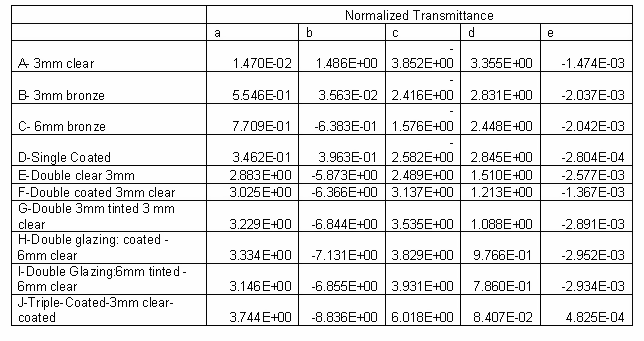
\includegraphics[width=0.9\textwidth, height=0.9\textheight, keepaspectratio=true]{media/image950.png}
\caption{Normalized Transmittance Correlations for Angular Performance \protect \label{fig:normalized-transmittance-correlations-for}}
\end{figure}

\begin{figure}[hbtp] % fig 76
\centering
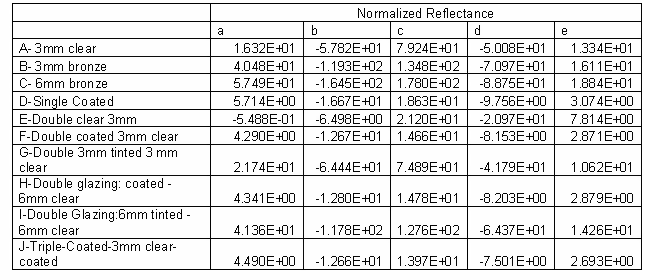
\includegraphics[width=0.9\textwidth, height=0.9\textheight, keepaspectratio=true]{media/image951.png}
\caption{Normalized Reflectanct Correlations for Angular Performance \protect \label{fig:normalized-reflectanct-correlations-for}}
\end{figure}

\subsubsection{Application Issues}\label{application-issues}

EnergyPlus's normal process of running the detailed layer-by-layer model, with the equivalent layer produced by this model, creates reports (sent to the EIO file) of the overall performance indices and the properties of the equivalent layer. Both of these raise issues that may be confusing.

The simplified window model does not reuse all aspects of the detailed layer-by-layer model, in that the angular solar transmission properties use a different model when the simple window model is in effect. If the user takes the material properties of an equivalent glazing layer from the simple window model and then re-enters them into just the detailed model, then the performance will not be the same because of the angular transmission model will have changed. It is not proper use of the model to re-enter the equivalent layer's properties and expect the exact level of performance.

There may not be exact agreement between the performance indices echoed out and those input in the model. This is expected with the model and the result of a number of factors. For example, although input is allowed to go up to U-7 W/m\(^{2}\)∙K, the actual outcome is limited to no higher than about 5.8W/m\(^{2}\)∙K. This is because the thermal resistance to heat transfer at the surfaces is already enough resistance to provide an upper limit to the conductance of a planar surface. Sometimes there is conflict between the SHGC and the U that are not physical and compromises need to be made. In general, the simple window model is intended to generate a physically-reasonable glazing that approximates the input entered as well as possible. But the model is not always be able to do exactly what is specified when the specifications are not physical.

\subsubsection{References}\label{references-054}

Arasteh, D., J.C. Kohler, B. Griffith, Modeling Windows in EnergyPlus with Simple Performance Indices. Lawrence Berkeley National Laboratory. In Draft. Available at

\subsection{Glazing System Properties}\label{glazing-system-properties}

The optical properties of a glazing system consisting of \emph{N} glass layers separated by nonabsorbing gas layers (Figure~\ref{fig:schematic-of-transmission-reflection}.~ Schematic of transmission, reflection and absorption of solar radiation within a multi-layer glazing system.) are determined by solving the following recursion relations for \emph{T\(_{i,j}\)}, the transmittance through layers* i* to* j\emph{;}R\(^{f}\)\(_{i,j}\)* and \emph{R\(^{b}\)\(_{i,j}\)}, the front and back reflectance, respectively, from layers* i* to* j\emph{; and}A\(_{j}\)\emph{, the absorption in layer} j\emph{. Here layer 1 is the outermost layer and layer}N* is the innermost layer. These relations account for multiple internal reflections within the glazing system. Each of the variables is a function of wavelength.

\begin{equation}
{T_{i,j}} = \frac{{{T_{i,j - 1}}{T_{j,j}}}}{{1 - R_{j,j}^fR_{j - 1,i}^b}}
\end{equation}

\begin{equation}
R_{i,j}^f = R_{i,j - 1}^f + \frac{{T_{i,j - 1}^2R_{j,j}^f}}{{1 - R_{j,j}^fR_{j - 1,i}^b}}
\end{equation}

\begin{equation}
R_{j,i}^b = R_{j,j}^b + \frac{{T_{j,j}^2R_{j - 1,i}^b}}{{1 - R_{j - 1,i}^bR_{j,j}^f}}
\end{equation}

\begin{equation}
A_j^f = \frac{{{T_{1,j - 1}}(1 - {T_{j,j}} - R_{j,j}^f)}}{{1 - R_{j,N}^fR_{j - 1,1}^b}} + \frac{{{T_{1,j}}R_{j + 1,N}^f(1 - {T_{j,j}} - R_{j,j}^b)}}{{1 - R_{j,N}^fR_{j - 1,1}^b}}
\end{equation}

In Eq. \emph{T\(_{i,j}\)} = 1 and \emph{R\(_{i,j}\)} = 0 if* i\emph{\textless{}0 or} j\emph{\textgreater{}}N*.

\begin{figure}[hbtp] % fig 77
\centering
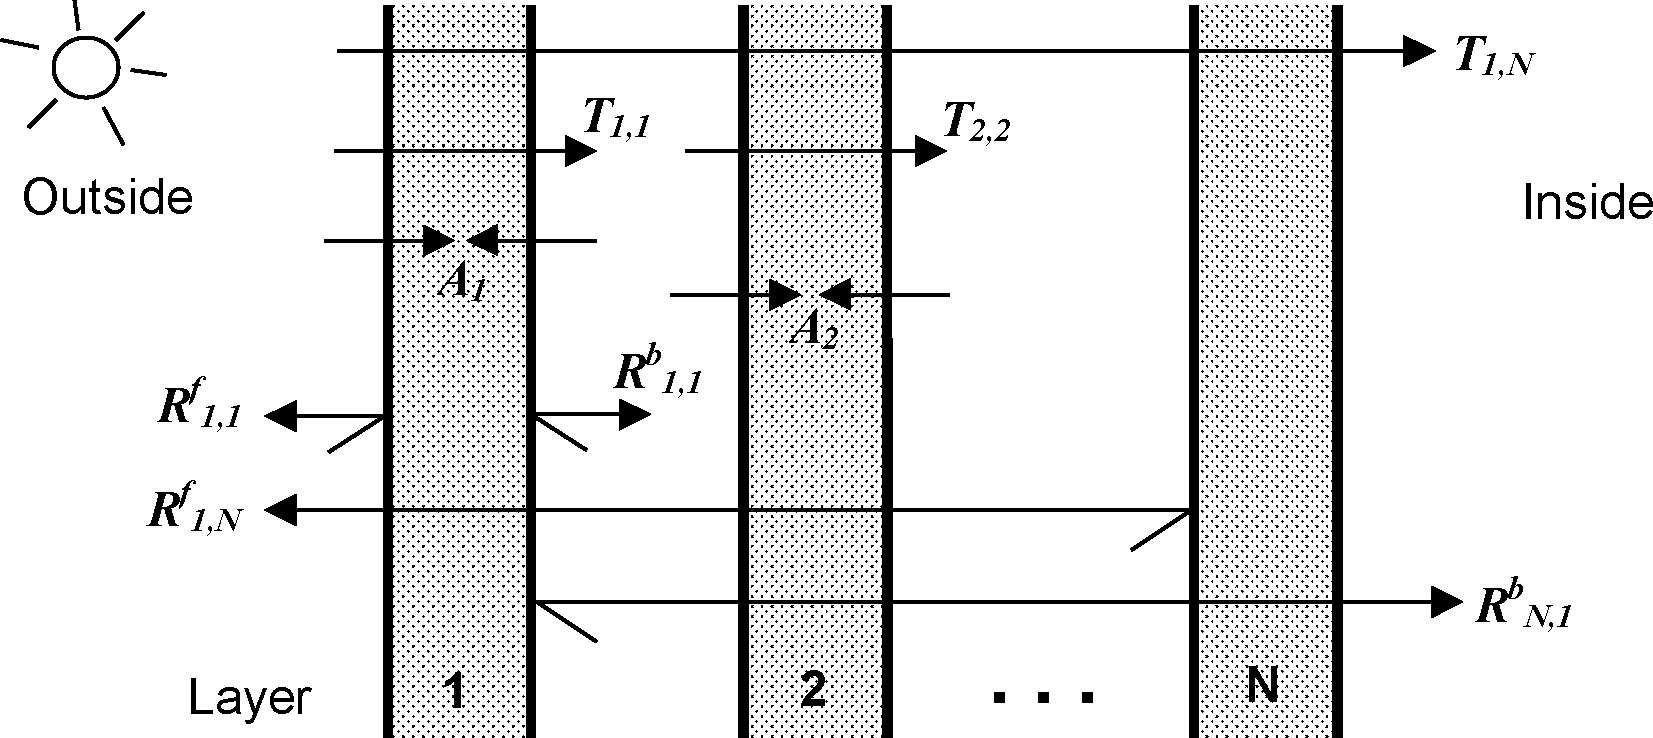
\includegraphics[width=0.9\textwidth, height=0.9\textheight, keepaspectratio=true]{media/image956.png}
\caption{Schematic of transmission, reflection and absorption of solar radiation within a multi-layer glazing system. \protect \label{fig:schematic-of-transmission-reflection}}
\end{figure}

As an example, for double glazing (\emph{N} = 2) these equations reduce to

\begin{equation}
{T_{1,2}} = \frac{{{T_{1,1}}{T_{2,2}}}}{{1 - R_{2,2}^fR_{1,1}^b}}
\end{equation}

\begin{equation}
R_{1,2}^f = R_{1,1}^f + \frac{{T_{1,1}^2R_{2,2}^f}}{{1 - R_{2,2}^fR_{1,1}^b}}
\end{equation}

\begin{equation}
R_{2,1}^b = R_{2,2}^b + \frac{{T_{2,2}^2R_{1,1}^b}}{{1 - R_{1,1}^bR_{2,2}^f}}
\end{equation}

\begin{equation}
A_1^f = (1 - {T_{1,1}} - R_{1,1}^f) + \frac{{{T_{1,1}}R_{2,2}^f(1 - {T_{1,1}} - R_{1,1}^b)}}{{1 - R_{2,2}^fR_{1,1}^b}}
\end{equation}

\begin{equation}
A_2^f = \frac{{{T_{1,1}}(1 - {T_{2,2}} - R_{2,2}^f)}}{{1 - R_{2,2}^fR_{1,1}^b}}
\end{equation}

If the above transmittance and reflectance properties are input as a function of wavelength, EnergyPlus calculates ``spectral average'' values of the above glazing system properties by integrating over wavelength:

The spectral-average solar property is

\begin{equation}
{P_s} = \frac{{\int {P(\lambda ){E_s}(\lambda )d\lambda } }}{{\int {{E_s}(\lambda )d\lambda } }}
\end{equation}

The spectral-average visible property is

\begin{equation}
{P_v} = \frac{{\int {P(\lambda ){E_s}(\lambda )V(\lambda )d\lambda } }}{{\int {{E_s}(\lambda )V(\lambda )d\lambda } }}
\end{equation}

where \({E_s}(\lambda )\) is the solar spectral irradiance function and \(V(\lambda )\) is the photopic response function of the eye. The default functions are shown in Table~\ref{table:solar-spectral-irradiance-function.} and Table~\ref{table:photopic-response-function.}. They can be overwritten by user defined solar and/or visible spectrum using the objects Site:SolarAndVisibleSpectrum and Site:SpectrumData. They are expressed as a set of values followed by the corresponding wavelengths for values.

If a glazing layer has optical properties that are roughly constant with wavelength, the wavelength-dependent values of \emph{T\(_{i,i}\)} , \emph{R\(^{f}\)\(_{i,i}\)} and \emph{R\(^{b}\)\(_{i,i}\)} in Eqs. to can be replaced with constant values for that layer.

% table 29
\begin{longtable}[c]{p{0.5in}p{0.5in}p{0.5in}p{0.5in}p{0.5in}p{0.5in}p{0.5in}p{0.5in}p{0.5in}p{0.5in}}

\caption{Solar spectral irradiance function. \label{table:solar-spectral-irradiance-function.}} \tabularnewline
\toprule 
\endfirsthead

\caption[]{Solar spectral irradiance function.} \tabularnewline
\toprule 
\endhead

\multicolumn{10}{l}{Air mass 1.5 terrestrial solar global spectral irradiance values (W/m-micron) on a 37 tilted surface.} \tabularnewline
\multicolumn{10}{l}{Corresponds to wavelengths in following data block. Based on ISO 9845-1 and ASTM E 892;} \tabularnewline
\multicolumn{10}{l}{derived from Optics5 data file ISO-9845GlobalNorm.std, 10-14-99.} \tabularnewline
\midrule
\endhead
0.0, & 9.5, & 42.3, & 107.8, & 181.0, & 246.0, & 395.3, & 390.1, & 435.3, & 438.9, \tabularnewline 
483.7, & 520.3, & 666.2, & 712.5, & 720.7, & 1013.1, & 1158.2, & 1184.0, & 1071.9, & 1302.0, \tabularnewline 
1526.0, & 1599.6, & 1581.0, & 1628.3, & 1539.2, & 1548.7, & 1586.5, & 1484.9, & 1572.4, & 1550.7, \tabularnewline 
1561.5, & 1501.5, & 1395.5, & 1485.3, & 1434.1, & 1419.9, & 1392.3, & 1130.0, & 1316.7, & 1010.3, \tabularnewline 
1043.2, & 1211.2, & 1193.9, & 1175.5, & 643.1, & 1030.7, & 1131.1, & 1081.6, & 849.2, & 785.0, \tabularnewline 
916.4, & 959.9, & 978.9, & 933.2, & 748.5, & 667.5, & 690.3, & 403.6, & 258.3, & 313.6, \tabularnewline 
526.8, & 646.4, & 746.8, & 690.5, & 637.5, & 412.6, & 108.9, & 189.1, & 132.2, & 339.0, \tabularnewline 
460.0, & 423.6, & 480.5, & 413.1, & 250.2, & 32.5, & 1.6, & 55.7, & 105.1, & 105.5, \tabularnewline 
182.1, & 262.2, & 274.2, & 275.0, & 244.6, & 247.4, & 228.7, & 244.5, & 234.8, & 220.5, \tabularnewline 
171.5, & 30.7, & 2.0, & 1.2, & 21.2, & 91.1, & 26.8, & 99.5, & 60.4, & 89.1, \tabularnewline 
82.2, & 71.5, & 70.2, & 62.0, & 21.2, & 18.5, & 3.2 \tabularnewline \midrule
\multicolumn{10}{l}{Wavelengths (microns) corresponding to above data block} \tabularnewline \midrule
0.3000, & 0.3050, & 0.3100, & 0.3150, & 0.3200, & 0.3250, & 0.3300, & 0.3350, & 0.3400, & 0.3450, \tabularnewline 
0.3500, & 0.3600, & 0.3700, & 0.3800, & 0.3900, & 0.4000, & 0.4100, & 0.4200, & 0.4300, & 0.4400, \tabularnewline  
0.4500, & 0.4600, & 0.4700, & 0.4800, & 0.4900, & 0.5000, & 0.5100, & 0.5200, & 0.5300, & 0.5400, \tabularnewline
0.5500, & 0.5700, & 0.5900, & 0.6100, & 0.6300, & 0.6500, & 0.6700, & 0.6900, & 0.7100, & 0.7180, \tabularnewline
0.7244, & 0.7400, & 0.7525, & 0.7575, & 0.7625, & 0.7675, & 0.7800, & 0.8000, & 0.8160, & 0.8237, \tabularnewline
0.8315, & 0.8400, & 0.8600, & 0.8800, & 0.9050, & 0.9150, & 0.9250, & 0.9300, & 0.9370, & 0.9480, \tabularnewline
0.9650, & 0.9800, & 0.9935, & 1.0400, & 1.0700, & 1.1000, & 1.1200, & 1.1300, & 1.1370, & 1.1610, \tabularnewline
1.1800, & 1.2000, & 1.2350, & 1.2900, & 1.3200, & 1.3500, & 1.3950, & 1.4425, & 1.4625, & 1.4770, \tabularnewline
1.4970, & 1.5200, & 1.5390, & 1.5580, & 1.5780, & 1.5920, & 1.6100, & 1.6300, & 1.6460, & 1.6780, \tabularnewline
1.7400, & 1.8000, & 1.8600, & 1.9200, & 1.9600, & 1.9850, & 2.0050, & 2.0350, & 2.0650, & 2.1000, \tabularnewline
2.1480, & 2.1980, & 2.2700, & 2.3600, & 2.4500, & 2.4940, & 2.5370 \tabularnewline
\bottomrule
\end{longtable}

% table 30
\begin{longtable}[c]{p{0.5in}p{0.5in}p{0.5in}p{0.5in}p{0.5in}p{0.5in}p{0.5in}p{0.5in}p{0.5in}p{0.5in}}

\caption{Photopic response function. \label{table:photopic-response-function.}} \tabularnewline
\toprule 
\endfirsthead

\caption[]{Photopic response function.} \tabularnewline
\toprule 
\endhead

\multicolumn{10}{l}{Photopic response function values corresponding to wavelengths in following data block.} \tabularnewline 
\multicolumn{10}{l}{Based on CIE 1931 observer; ISO/CIE 10527, CIE Standard Calorimetric Observers;} \tabularnewline 
\multicolumn{10}{l}{derived from Optics5 data file "CIE 1931 Color Match from E308.txt",} \tabularnewline 
\multicolumn{10}{l}{which is the same as WINDOW4 file Cie31t.dat.} \tabularnewline \midrule \endhead
0.0000, & 0.0001, & 0.0001, & 0.0002, & 0.0004, & 0.0006, & 0.0012, & 0.0022, & 0.0040, & 0.0073, \tabularnewline 
0.0116, & 0.0168, & 0.0230, & 0.0298, & 0.0380, & 0.0480, & 0.0600, & 0.0739, & 0.0910, & 0.1126, \tabularnewline 
0.1390, & 0.1693, & 0.2080, & 0.2586, & 0.3230, & 0.4073, & 0.5030, & 0.6082, & 0.7100, & 0.7932, \tabularnewline 
0.8620, & 0.9149, & 0.9540, & 0.9803, & 0.9950, & 1.0000, & 0.9950, & 0.9786, & 0.9520, & 0.9154, \tabularnewline 
0.8700, & 0.8163, & 0.7570, & 0.6949, & 0.6310, & 0.5668, & 0.5030, & 0.4412, & 0.3810, & 0.3210, \tabularnewline 
0.2650, & 0.2170, & 0.1750, & 0.1382, & 0.1070, & 0.0816, & 0.0610, & 0.0446, & 0.0320, & 0.0232, \tabularnewline 
0.0170, & 0.0119, & 0.0082, & 0.0158, & 0.0041, & 0.0029, & 0.0021, & 0.0015, & 0.0010, & 0.0007, \tabularnewline 
0.0005, & 0.0004, & 0.0002, & 0.0002, & 0.0001, & 0.0001, & 0.0001, & 0.0000, & 0.0000, & 0.0000, \tabularnewline 
0.0000 \tabularnewline \midrule
\multicolumn{10}{l}{Wavelengths (microns) corresponding to above data block} \tabularnewline \midrule
.380, & .385, & .390, & .395, & .400, & .405, & .410, & .415, & .420, & .425, \tabularnewline 
.430, & .435, & .440, & .445, & .450, & .455, & .460, & .465, & .470, & .475, \tabularnewline 
.480, & .485, & .490, & .495, & .500, & .505, & .510, & .515, & .520, & .525, \tabularnewline 
.530, & .535, & .540, & .545, & .550, & .555, & .560, & .565, & .570, & .575, \tabularnewline 
.580, & .585, & .590, & .595, & .600, & .605, & .610, & .615, & .620, & .625, \tabularnewline 
.630, & .635, & .640, & .645, & .650, & .655, & .660, & .665, & .670, & .675, \tabularnewline 
.680, & .685, & .690, & .695, & .700, & .705, & .710, & .715, & .720, & .725, \tabularnewline 
.730, & .735, & .740, & .745, & .750, & .755, & .760, & .765, & .770, & .775, \tabularnewline 
.780 \tabularnewline
\bottomrule
\end{longtable}

\subsection{Calculation of Angular Properties}\label{calculation-of-angular-properties}

Calculation of optical properties is divided into two categories: uncoated glass and coated glass.

\subsubsection{Angular Properties for Uncoated Glass}\label{angular-properties-for-uncoated-glass}

The following discussion assumes that optical quantities such as transmissivity, reflectvity, absorptivity, and index of refraction are a function of wavelength, λ. If there are no spectral data the angular dependence is calculated based on the single values for transmittance and reflectance in the visible and solar range. In the visible range an average wavelength of 0.575 microns is used in the calculations. In the solar range an average wavelength of 0.898 microns is used.

The spectral data include the transmittance, \emph{T}, and the reflectance, \emph{R}. For uncoated glass the reflectance is the same for the front and back surfaces. For angle of incidence, \(\phi\) , the transmittance and reflectance are related to the transmissivity, τ,and reflectivity, ρ, by the following relationships:

\begin{equation}
T(\phi ) = \frac{{\tau {{(\phi )}^2}{e^{ - \alpha d/\cos \phi '}}}}{{1 - \rho {{(\phi )}^2}{e^{ - 2\alpha d/\cos \phi '}}}}
\end{equation}

\begin{equation}
R(\phi ) = \rho (\phi )\left( {1 + T(\phi ){e^{ - \alpha d/\cos \phi '}}} \right)
\end{equation}

The spectral reflectivity is calculated from Fresnel's equation assuming unpolarized incident radiation:

\begin{equation}
\rho (\phi ) = \frac{1}{2}\left( {{{\left( {\frac{{n\cos \phi  - \cos \phi '}}{{n\cos \phi  + \cos \phi '}}} \right)}^2} + {{\left( {\frac{{n\cos \phi ' - \cos \phi }}{{n\cos \phi ' + \cos \phi }}} \right)}^2}} \right)
\end{equation}

The spectral transmittivity is given by

\begin{equation}
\tau (\phi ) = 1 - \rho (\phi )
\end{equation}

The spectral absorption coefficient is defined as

\begin{equation}
\alpha  = 4\pi \kappa /\lambda
\end{equation}

where κ is the dimensionless spectrally-dependent extinction coefficient and λ is the wavelength expressed in the same units as the sample thickness.

Solving Eq. at normal incidence gives

\begin{equation}
n = \frac{{1 + \sqrt {\rho (0)} }}{{1 - \sqrt {\rho (0)} }}
\end{equation}

Evaluating Eq. at normal incidence gives the following expression for \emph{κ}

\begin{equation}
\kappa  =  - \frac{\lambda }{{4\pi d}}\ln \frac{{R(0) - \rho (0)}}{{\rho (0)T(0)}}
\end{equation}

Eliminating the exponential in Eqs. and~ gives the reflectivity at normal incidence:

\begin{equation}
\rho (0) = \frac{{\beta  - \sqrt {{\beta ^2} - 4(2 - R(0))R(0)} }}{{2(2 - R(0))}}
\end{equation}

where

\begin{equation}
\beta  = T{(0)^2} - R{(0)^2} + 2R(0) + 1
\end{equation}

The value for the reflectivity, \emph{ρ}(0),from Eq. is substituted into Eqs. and . The result from Eq. is used to calculate the absorption coefficient in Eq. . The index of refraction is used to calculate the reflectivity in Eq. which is then used to calculate the transmittivity in Eq. . The reflectivity, transmissivity and absorption coefficient are then substituted into Eqs. and to obtain the angular values of the reflectance and transmittance.

\subsubsection{Angular Properties for Coated Glass}\label{angular-properties-for-coated-glass}

A regression fit is used to calculate the angular properties of coated glass from properties at normal incidence. If the transmittance of the coated glass is \textgreater{} 0.645, the angular dependence of uncoated clear glass is used. If the transmittance of the coated glass is ≤ 0.645, the angular dependence of uncoated bronze glass is used. The values for the angular functions for the transmittance and reflectance of both clear glass \(({\bar \tau_{clr}},{\bar \rho_{clr}})\) ~and bronze glass \(({\bar \tau_{bnz}},{\bar \rho_{bnz}})\) are determined from a fourth-order polynomial regression:

\begin{equation}
\bar \tau (\phi ) = {\bar \tau_0} + {\bar \tau_1}\cos (\phi ) + {\bar \tau_2}{\cos ^2}(\phi ) + {\bar \tau_3}{\cos ^3}(\phi ) + {\bar \tau_4}{\cos ^4}(\phi )
\end{equation}

and

\begin{equation}
\bar \rho (\phi ) = {\bar \rho_0} + {\bar \rho_1}\cos (\phi ) + {\bar \rho_2}{\cos ^2}(\phi ) + {\bar \rho_3}{\cos ^3}(\phi ) + {\bar \rho_4}{\cos ^4}(\phi ) - \bar \tau (\phi )
\end{equation}

The polynomial coefficients are given in Table~\ref{table:polynomial-coefficients-used-to-determine}.

% table 31
\begin{longtable}[c]{p{1.0in}p{1.0in}p{1.0in}p{1.0in}p{1.0in}p{1.0in}}

\caption{Polynomial coefficients used to determine angular properties of coated glass. \label{table:polynomial-coefficients-used-to-determine}} \tabularnewline
\toprule 
~ & 0 & 1 & 2 & 3 & 4 \tabularnewline
\midrule
\endfirsthead

\caption[]{Polynomial coefficients used to determine angular properties of coated glass.} \tabularnewline
\toprule 
~ & 0 & 1 & 2 & 3 & 4 \tabularnewline
\midrule
\endhead

$\bar{\tau}_{clr}$ & -0.0015 & 3.355 & -3.840 & 1.460 & 0.0288 \tabularnewline
$\bar{\rho}_{clr}$ & 0.999 & -0.563 & 2.043 & -2.532 & 1.054 \tabularnewline
$\bar{\tau}_{bnz}$ & -0.002 & 2.813 & -2.341 & -0.05725 & 0.599 \tabularnewline
$\bar{\rho}_{bnz}$ & 0.997 & -1.868 & 6.513 & -7.862 & 3.225 \tabularnewline
\bottomrule
\end{longtable}

These factors are used as follows to calculate the angular transmittance and reflectance:

For \emph{T}(0) \textgreater{} 0.645:

\begin{equation}
T(\phi ) = T(0){\bar \tau_{clr}}(\phi )
\end{equation}

\begin{equation}
R(\phi ) = R(0)(1 - {\bar \rho_{clr}}(\phi )) + {\bar \rho_{clr}}(\phi )
\end{equation}

For \emph{T}(0) ≤ 0.645:

\begin{equation}
T(\phi ) = T(0){\bar \tau_{bnz}}(\phi )
\end{equation}

\begin{equation}
R(\phi ) = R(0)(1 - {\bar \rho_{bnz}}(\phi )) + {\bar \rho_{bnz}}(\phi )
\end{equation}

\subsubsection{Angular Properties for Simple Glazing Systems}\label{angular-properties-for-simple-glazing-systems}

When the glazing system is modeled using the simplified method, an alternate method is used to determine the angular properties.~ The equation for solar transmittance as a function of incidence angle, \(T\left( \phi \right)\) , is,

\begin{equation}
T\left( \phi  \right) = T\left( {\phi  = 0} \right)\,\cos \left( \phi  \right)\,\,\left( {1 + (0.768 + 0.817\,SHG{C^4})\;{{\sin }^3}\left( \phi  \right)} \right)
\end{equation}

where,

\(T\left( {\phi = 0} \right)\) ~is the normal incidence solar transmittance, \({T_{Sol}}\) .

The equation for solar reflectance as a function of incidence angle,~ \(R\left( \phi \right)\) , is,

\begin{equation}
R\left( \phi  \right) = \frac{{R\left( {\phi  = 0} \right)\left( {{f_1}\left( \phi  \right) + {f_2}\left( \phi  \right)\sqrt {SHGC} } \right)}}{{{R_{fit,o}}}}
\end{equation}

where,

\begin{equation}
{f_1}\left( \phi  \right) = \left( {\left( {\left( {2.403\cos \left( \phi  \right) - 6.192} \right)\cos \left( \phi  \right) + 5.625} \right)\cos \left( \phi  \right) - 2.095} \right)\cos \left( \phi  \right) + 1
\end{equation}

\begin{equation}
{f_2}\left( \phi  \right) = \left( {\left( {\left( { - 1.188\cos \left( \phi  \right) + 2.022} \right)\cos \left( \phi  \right) + 0.137} \right)\cos \left( \phi  \right) - 1.720} \right)\cos \left( \phi  \right)
\end{equation}

\begin{equation}
{R_{fit,o}} = 0.7413 - \left( {0.7396\;\sqrt {SHGC} } \right)
\end{equation}

\subsection{Calculation of Hemispherical Values}\label{calculation-of-hemispherical-values}

The hemispherical value of a property is determined from the following integral:

\begin{equation}
{P_{hemispherical}} = 2\int_0^{\frac{\pi }{2}} {P(\phi )\cos (\phi )\sin (\phi )d\phi }
\end{equation}

The integral is evaluated by Simpson's rule for property values at angles of incidence from 0 to 90 degrees in 10-degree increments.

\subsection{Optical Properties of Window Shading Devices}\label{optical-properties-of-window-shading-devices}

Shading devices affect the system transmittance and glass layer absorptance for short-wave radiation and for long-wave (thermal) radiation. The effect depends on the shade position (interior, exterior or between-glass), its transmittance, and the amount of inter-reflection between the shading device and the glazing. Also of interest is the amount of radiation absorbed by the shading device.

In EnergyPlus, shading devices are divided into four categories, ``shades,'' ''blinds,'' ``screens,'' and ``switchable glazing.'' ``Shades'' are assumed to be perfect diffusers. This means that direct radiation incident on the shade is reflected and transmitted as hemispherically uniform diffuse radiation: there is no direct component of transmitted radiation. It is also assumed that the transmittance, \emph{τ\(_{sh}\)}, reflectance, \emph{ρ\(_{sh}\)}, and absorptance, \emph{α\(_{sh}\)}, are the same for the front and back of the shade and are independent of angle of incidence. Many types of drapery and pull-down roller devices are close to being perfect diffusers and can be categorized as ``shades.''

``Blinds'' in EnergyPlus are slat-type devices such as venetian blinds. Unlike shades, the optical properties of blinds are strongly dependent on angle of incidence. Also, depending on slat angle and the profile angle of incident direct radiation, some of the direct radiation may pass between the slats, giving a direct component of transmitted radiation.

``Screens'' are debris or insect protection devices made up of metallic or non-metallic materials. Screens may also be used as shading devices for large glazing areas where excessive solar gain is an issue. The EnergyPlus window screen model assumes the screen is composed of intersecting orthogonally-crossed cylinders, with the surface of the cylinders assumed to be diffusely reflecting. Screens may only be used on the exterior surface of a window construction. As with blinds, the optical properties affecting the direct component of transmitted radiation are dependent on the angle of incident direct radiation.

With ``Switchable glazing,'' shading is achieved making the glazing more absorbing or more reflecting, usually by an electrical or chemical mechanism. An example is electrochromic glazing where the application of an electrical voltage or current causes the glazing to switch from light to dark.

Shades and blinds can be either fixed or moveable. If moveable, they can be deployed according to a schedule or according to a trigger variable, such as solar radiation incident on the window. Screens can be either fixed or moveable according to a schedule.

\subsubsection{Shades}\label{shades}

\subsubsection{Shade/Glazing System Properties for Short-Wave Radiation}\label{shadeglazing-system-properties-for-short-wave-radiation}

Short-wave radiation includes

1)~~~Beam solar radiation from the sun and diffuse solar radiation from the sky and ground incident on the outside of the window,

2)~~~Beam and/or diffuse radiation reflected from exterior obstructions or the building itself,

3)~~~Solar radiation reflected from the inside zone surfaces and incident as diffuse radiation on the inside of the window,

4)~~~Beam solar radiation from one exterior window incident on the inside of another window in the same zone, and

5)~~~Short-wave radiation from electric lights incident as diffuse radiation on the inside of the window.

\textbf{Exterior Shade}

For an exterior shade we have the following expressions for the system transmittance, the effective system glass layer absorptance, and the system shade absorptance, taking inter-reflection between shade and glazing into account. Here, ``system'' refers to the combination of glazing and shade. The system properties are given in terms of the isolated shade properties (i.e., shade properties in the absence of the glazing) and the isolated glazing properties (i.e., glazing properties in the absence of the shade).

\begin{equation}
{T_{sys}}(\phi ) = T_{1,N}^{dif}\frac{{{\tau_{sh}}}}{{1 - R_f^{dif}{\rho_{sh}}}}
\end{equation}

\begin{equation}
T_{sys}^{dif} = T_{1,N}^{dif}\frac{{{\tau_{sh}}}}{{1 - R_f^{dif}{\rho_{sh}}}}
\end{equation}

\begin{equation}
A_{j,f}^{sys}(\phi ) = A_{j,f}^{dif}\frac{{{\tau_{sh}}}}{{1 - {R_f}{\rho_{sh}}}},\quad j = 1{\rm{to}}N
\end{equation}

\begin{equation}
A_{j,f}^{dif,sys} = A_{j,f}^{dif}\frac{{{\tau_{sh}}}}{{1 - {R_f}{\rho_{sh}}}},\quad j = 1{\rm{ to }}N
\end{equation}

\begin{equation}
A_{j,b}^{dif,sys} = A_{j,b}^{dif}\frac{{T_{1,N}^{dif}{\rho_{sh}}}}{{1 - {R_f}{\rho_{sh}}}},\quad j = 1{\rm{ to }}N
\end{equation}

\begin{equation}
\alpha_{sh}^{sys} = {\alpha_{sh}}\left( {1 + \frac{{{\tau_{sh}}{R_f}}}{{1 - {R_f}{\rho_{sh}}}}} \right)
\end{equation}

\textbf{Interior Shade}

The system properties when an interior shade is in place are the following.

\begin{equation}
{T_{sys}}(\phi ) = T_{1,N}^{}(\phi )\frac{{{\tau_{sh}}}}{{1 - R_b^{dif}{\rho_{sh}}}}
\end{equation}

\begin{equation}
T_{sys}^{dif} = T_{1,N}^{dif}\frac{{{\tau_{sh}}}}{{1 - R_b^{dif}{\rho_{sh}}}}
\end{equation}

\begin{equation}
A_{j,f}^{sys}(\phi ) = {A_{j,f}}(\phi ) + {T_{1,N}}(\phi )\frac{{{\rho_{sh}}}}{{1 - R_b^{dif}{\rho_{sh}}}}A_{j,b}^{dif},\quad j = 1{\rm{ to }}N
\end{equation}

\begin{equation}
A_{j,f}^{dif,sys} = A_{j,f}^{dif} + T_{1,N}^{dif}\frac{{{\rho_{sh}}}}{{1 - R_b^{dif}{\rho_{sh}}}}A_{j,b}^{dif},\quad j = 1{\rm{ to }}N
\end{equation}

\begin{equation}
A_{j,b}^{dif,sys} = \frac{{{\tau_{sh}}}}{{1 - R_b^{dif}{\rho_{sh}}}}A_{j,b}^{dif},{\rm{    }}j = 1{\rm{ to }}N
\end{equation}

\begin{equation}
\alpha_{sh}^{sys}(\phi ) = T_{1,N}^{}(\phi )\frac{{{\alpha_{sh}}}}{{1 - R_b^{dif}{\rho_{sh}}}}
\end{equation}

\begin{equation}
\alpha_{sh}^{dif,sys} = T_{1,N}^{dif}\frac{{{\alpha_{sh}}}}{{1 - R_b^{dif}{\rho_{sh}}}}
\end{equation}

\subsubsection{Long-Wave Radiation Properties of Window Shades}\label{long-wave-radiation-properties-of-window-shades}

Long-wave radiation includes

~~~~~~~Thermal radiation from the sky, ground and exterior obstructions incident on the outside of the window,

~~~~~~~Thermal radiation from other room surfaces incident on the inside of the window, and

~~~~~~~Thermal radiation from internal sources, such as equipment and electric lights, incident on the inside of the window.

The program calculates how much long-wave radiation is absorbed by the shade and by the adjacent glass surface. The system emissivity (thermal absorptance) for an interior or exterior shade, taking into account reflection of long-wave radiation between the glass and shade, is given by

\begin{equation}
\varepsilon_{sh}^{lw,sys} = \varepsilon_{sh}^{lw}\left( {1 + \frac{{\tau_{sh}^{lw}\rho_{gl}^{lw}}}{{1 - \rho_{sh}^{lw}\rho_{gl}^{lw}}}} \right)
\end{equation}

where \(\rho_{gl}^{lw}\) is the long-wave reflectance of the outermost glass surface for an exterior shade or the innermost glass surface for an interior shade, and it is assumed that the long-wave transmittance of the glass is zero.

The innermost (for interior shade) or outermost (for exterior shade) glass surface emissivity when the shade is present is

\begin{equation}
\varepsilon_{gl}^{lw,sys} = \varepsilon_{gl}^{lw}\frac{{\tau_{sh}^{lw}}}{{1 - \rho_{sh}^{lw}\rho_{gl}^{lw}}}
\end{equation}

\subsubsection{Switchable Glazing}\label{switchable-glazing}

For switchable glazing, such as electrochromics, the solar and visible optical properties of the glazing can switch from a light state to a dark state. The switching factor, \emph{f\(_{switch}\)}, determines what state the glazing is in. An optical property, \emph{p}, such as transmittance or glass layer absorptance, for this state is given by

\begin{equation}
p = (1 - {f_{switch}}){p_{light}} + {f_{switch}}{p_{dark}}
\end{equation}

where

\emph{p\(_{light}\)}is the property value for the unswitched, or light state, and \emph{p\(_{dark}\)} is the property value for the fully switched, or dark state.

The value of the switching factor in a particular time step depends on what type of switching control has been specified: ``schedule,'' ``trigger,'' or ``daylighting.'' If ``schedule,'' \emph{f\(_{switch}\)} = schedule value, which can be 0 or 1.

\subsection{Thermochromic Windows}\label{thermochromic-windows}

Thermochromic (TC) materials have active, reversible optical properties that vary with temperature. Thermochromic windows are adaptive window systems for incorporation into building envelopes. Thermochromic windows respond by absorbing sunlight and turning the sunlight energy into heat. As the thermochromic film warms it changes its light transmission level from less absorbing to more absorbing. The more sunlight it absorbs the lower the light level going through it. Figure~\ref{fig:variations-of-window-properties-with} shows the variations of window properties with the temperature of the thermochromic glazing layer. By using the suns own energy the window adapts based solely on the directness and amount of sunlight. Thermochromic materials will normally reduce optical transparency by absorption and/or reflection, and are specular (maintaining vision).

\begin{figure}[hbtp] % fig 78
\centering
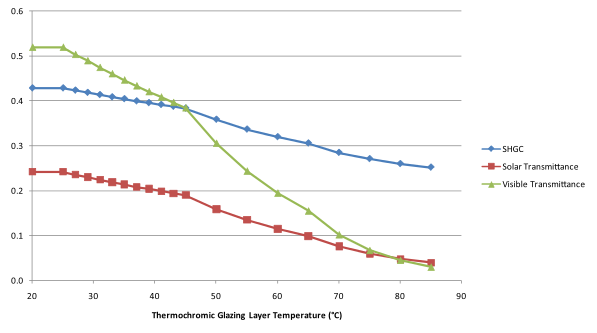
\includegraphics[width=0.9\textwidth, height=0.9\textheight, keepaspectratio=true]{media/image1015.svg.png}
\caption{Variations of Window Properties with the Temperature of the Thermochromic Glazing Layer \protect \label{fig:variations-of-window-properties-with}}
\end{figure}

On cloudy days the window is at full transmission and letting in diffuse daylighting. On sunny days the window maximizes diffuse daylighting and tints based on the angle of the sun relative to the window. For a south facing window (northern hemisphere) the daylight early and late in the day is maximized and the direct sun at mid day is minimized.

The active thermochromic material can be embodied within a laminate layer or a surface film. The overall optical state of the window at a given time is a function primarily of

\begin{itemize}
\item
  thermochromic material properties
\item
  solar energy incident on the window
\item
  construction of the window system that incorporates the thermochromic layer
\item
  environmental conditions (interior, exterior, air temperature, wind, etc).
\end{itemize}

The tinted film, in combination with a heat reflecting, low-e layer allows the window to reject most of the absorbed radiation thus reducing undesirable heat load in a building. In the absence of direct sunlight the window cools and clears and again allows lower intensity diffuse radiation into a building. TC windows can be designed in several ways (Figure~\ref{fig:configurations-of-thermochromic-windows}), with the most common being a triple pane windows with the TC glass layer in the middle a double pane windows with the TC layer on the inner surface of the outer pane or for sloped glazing a double pane with the laminate layer on the inner pane with a low-e layer toward the interior. The TC glass layer has variable optical properties depending on its temperature, with a lower temperature at which the optical change is initiated, and an upper temperature at which a minimum transmittance is reached. TC windows act as passive solar shading devices without the need for sensors, controls and power supplies but their optical performance is dependent on varying solar and other environmental conditions at the location of the window.

\begin{figure}[hbtp] % fig 79
\centering
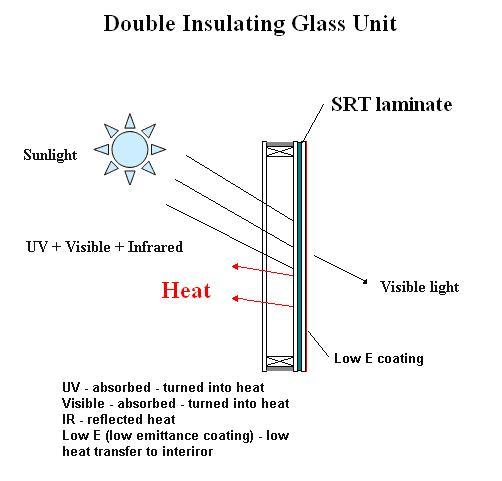
\includegraphics[width=0.9\textwidth, height=0.9\textheight, keepaspectratio=true]{media/image1017.png}
\caption{Configurations of Thermochromic Windows \protect \label{fig:configurations-of-thermochromic-windows}}
\end{figure}

EnergyPlus describes a thermochromic window with a Construction object which references a special layer defined with a WindowMaterial:GlazingGroup:Thermochromic object. The WindowMaterial:GlazingGroup:Thermochromic object further references a series of WindowMaterial:Glazing objects corresponding to each specification temperature of the TC layer. During EnergyPlus run time, a series of TC windows corresponding to each specification temperature is created once. At the beginning of a particular time step calculations, the temperature of the TC glass layer from the previous time step is used to look up the most closed specification temperature whose corresponding TC window construction will be used for the current time step calculations. The current time step calculated temperature of the TC glass layer can be different from the previous time step, but no iterations are done in the current time step for the new TC glass layer temperature. This is an approximation that considers the reaction time of the TC glass layer can be close to EnergyPlus simulation time step say 10 to 15 minutes.

\subsubsection{Blinds}\label{blinds}

Window blinds in EnergyPlus are defined as a series of equidistant slats that are oriented horizontally or vertically. All of the slats are assumed to have the same optical properties. The overall optical properties of the blind are determined by the slat geometry (width, separation and angle) and the slat optical properties (front-side and back-side transmittance and reflectance). Blind properties for direct radiation are also sensitive to the ``profile angle,'' which is the angle of incidence in a plane that is perpendicular to the window plane and to the direction of the slats. The blind optical model in EnergyPlus is based on Simmler, Fischer and Winkelmann, 1996; however, that document has numerous typographical errors and should be used with caution.

The following assumptions are made in calculating the blind optical properties:

\begin{itemize}
\item
  The slats are flat.
\item
  The spectral dependence of inter-reflections between slats and glazing is ignored; spectral-average slat optical properties are used.
\item
  The slats are perfect diffusers. They have a perfectly matte finish so that reflection from a slat is isotropic (hemispherically uniform) and independent of angle of incidence, i.e., the reflection has no specular component. This also means that absorption by the slats is hemispherically uniform with no incidence angle dependence. If the transmittance of a slat is non-zero, the transmitted radiation is isotropic and the transmittance is independent of angle of incidence.
\item
  Inter-reflection between the blind and wall elements near the periphery of the blind is ignored.
\item
  If the slats have holes through which support strings pass, the holes and strings are ignored. Any other structures that support or move the slats are ignored.
\end{itemize}

\subsubsection{Slat Optical Properties}\label{slat-optical-properties}

The slat optical properties used by EnergyPlus are shown in the following table.

% table 32
\begin{longtable}[c]{p{1.5in}p{2.5in}}
\caption{Slat Optical Properties \label{table:slat-optical-properties}} \tabularnewline
\toprule 
\({\tau_{dir,dir}}\) & Direct-to-diffuse transmittance (same for front and back of slat) \tabularnewline
\midrule
\endfirsthead

\caption[]{Slat Optical Properties} \tabularnewline
\toprule
\({\tau_{dir,dir}}\) & Direct-to-diffuse transmittance (same for front and back of slat) \tabularnewline
\midrule
\endhead

\({\tau_{dir,dir}}\) & Direct-to-diffuse transmittance (same for front and back of slat) \tabularnewline
\({\tau_{dif,dir}}\) & Diffuse-to-diffuse transmittance (same for front and back of slat) \tabularnewline
\(\rho_{dir,dif}^f\), \(\rho_{dir,dif}^b\) & Front and back direct-to-diffuse reflectance \tabularnewline
\(\rho_{dif,dif}^f\), \(\rho_{dif,dif}^b\) & Front and back diffuse-to-diffuse reflectance \tabularnewline
\bottomrule
\end{longtable}

It is assumed that there is no direct-to-direct transmission or reflection, so that \({\tau_{dir,dir}} = 0\), \(\rho_{dir,dir}^f = 0\), and \(\rho_{dir,dir}^b = 0\). It is further assumed that the slats are perfect diffusers, so that \({\tau_{dir,dif}}\), \(\rho_{dir,dif}^f\) and \(\rho_{dir,dif}^b\) are independent of angle of incidence. Until the EnergyPlus model is improved to take into account the angle-of-incidence dependence of slat transmission and reflection, it is assumed that \({\tau_{dir,dif}}\) = \({\tau_{dif,dif}}\), \(\rho_{dir,dif}^f\) = \(\rho_{dif,dif}^f\), and \(\rho_{dir,dif}^b\) = \(\rho_{dif,dif}^b\).

\subsubsection{Direct Transmittance of Blind}\label{direct-transmittance-of-blind}

The direct-to-direct and direct-to-diffuse transmittance of a blind is calculated using the slat geometry shown in Figure~\ref{fig:a-side-view-of-a-cell-formed-by-adjacent} (a), which shows the side view of one of the cells of the blind. For the case shown, each slat is divided into two segments, so that the cell is bounded by a total of six segments, denoted by \emph{s\(_{1}\)} through \emph{s\(_{6}\)} (note in the following that \emph{s\(_{i}\)} refers to both segment \emph{i} and the length of segment \emph{i)}.The lengths of \emph{s\(_{1}\)} and \emph{s\(_{2}\)} are equal to the slat separation, \emph{h}, which is the distance between adjacent slat faces. \emph{s\(_{3}\)} and \emph{s\(_{4}\)} are the segments illuminated by direct radiation. In the case shown in Figure~\ref{fig:a-side-view-of-a-cell-formed-by-adjacent} (a) the cell receives radiation by reflection of the direct radiation incident on \emph{s\(_{4}\)} and, if the slats have non-zero transmittance, by transmission through \emph{s\(_{3}\)}, which is illuminated from above.

The goal of the blind direct transmission calculation is to determine the direct and diffuse radiation leaving the cell through \emph{s\(_{2}\)} for unit direct radiation entering the cell through \emph{s\(_{1}\)}.

\begin{figure}[hbtp] % fig 80
\centering
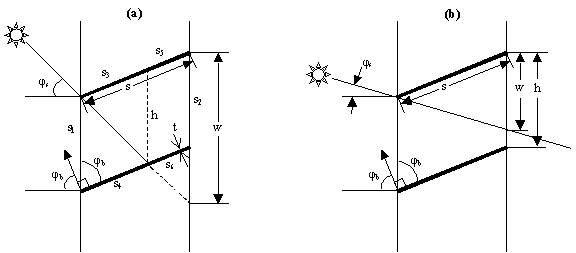
\includegraphics[width=0.9\textwidth, height=0.9\textheight, keepaspectratio=true]{media/image1034.png}
\caption{(a) Side view of a cell formed by adjacent slats showing how the cell is divided into segments, \(s_i\),  for the calculation of direct solar transmittance; (b) side view of a cell showing case where some of the direct solar passes between adjacent slats without touching either of them. In this figure \(\phi_s\) is the profile angle and \(\phi_b\) is the slat angle. \label{fig:a-side-view-of-a-cell-formed-by-adjacent}}
\end{figure}

\subsubsection{Direct-to-Direct Blind Transmittance}\label{direct-to-direct-blind-transmittance}

Figure~\ref{fig:a-side-view-of-a-cell-formed-by-adjacent} (b) shows the case where some of the direct radiation passes through the cell without hitting the slats. From the geometry in this figure we see that

\begin{equation}
\tau_{bl,f}^{dir,dir} = 1 - \frac{{|w|}}{h},{\rm{       }}|w|{\rm{ }} \le {\rm{ }}h
\end{equation}

where

\begin{equation}
w = s\frac{{\cos ({\varphi_b} - {\varphi_s})}}{{\cos {\varphi_s}}}
\end{equation}

Note that we are assuming that the slat thickness is zero. A correction for non-zero slat thickness is described later.

\subsubsection{Direct-to-Diffuse Blind Transmittance, Reflectance and Absorptance}\label{direct-to-diffuse-blind-transmittance-reflectance-and-absorptance}

The direct-to-diffuse and transmittance and reflectance of the blind are calculated using a radiosity method that involves the following three vector quantities:

\emph{J\(_{i}\)} = the radiosity of segment \emph{s\(_{i}\)}, i.e., the total radiant flux into the cell from~ \emph{s\(_{i}\)}

\emph{G\(_{i}\)} = the irradiance on the cell side of \emph{s\(_{i}\)}

\emph{Q\(_{i}\)} = the source flux from the cell side of s\emph{\(_{i}\)}

Based on these definitions we have the following equations that relate \emph{J}, \emph{G} and \emph{Q} for the different segments:

\begin{equation}
  \begin{array}{rl}
    J_1 & = Q_1 \\
    J_2 & = Q_2 \\
    J_3 & = Q_3 + \rho_{dif,dif}^b G_3 + \tau_{dif,dif} G_4 \\
    J_4 & = Q_4 + \tau_{dif,dif} G_3 + \rho_{dif,dif}^f G_4 \\
    J_5 & = Q_5 + \rho_{dif,dif}^b G_5 + \tau_{dif,dif} G_6 \\
    J_6 & = Q_6 + \tau_{dif,dif} G_5 + \rho_{dif,dif}^f G_6
  \end{array}
\end{equation}

In addition we have the following equation relating \emph{G} and* J*:

\begin{equation}
{G_i} = \sum\limits_{j = 1}^6 {{J_j}{F_{ji}}{\rm{ ,    }}i = 1,6}
\end{equation}

where \({F_{ji}}\) is the view factor between \({s_j}\) and \({s_i}\) , i.e., \({F_{ji}}\) is the fraction of radiation leaving \({s_j}\) that is intercepted by \({s_i}\) .

Using \({J_1} = {Q_1} = 0\) and \({J_2} = {Q_2} = 0\) ~and combining the above equations gives the following equation set relating* J* and* Q*:

\begin{equation}
{J_3} - \rho_{dif,dif}^b\sum\limits_{j = 3}^6 {{J_j}{F_{j3}} - {\tau_{dif,dif}}\sum\limits_{j = 3}^6 {{J_j}{F_{j4}} = {Q_3}} }
\end{equation}

\begin{equation}
{J_4} - \tau_{dif,dif}^{}\sum\limits_{j = 3}^6 {{J_j}{F_{j3}} - \rho_{dif,dif}^f\sum\limits_{j = 3}^6 {{J_j}{F_{j4}} = {Q_4}} }
\end{equation}

\begin{equation}
{J_5} - \rho_{dif,dif}^b\sum\limits_{j = 3}^6 {{J_j}{F_{j5}} - {\tau_{dif,dif}}\sum\limits_{j = 3}^6 {{J_j}{F_{j6}} = {Q_5}} }
\end{equation}

\begin{equation}
{J_6} - \tau_{dif,dif}^{}\sum\limits_{j = 3}^6 {{J_j}{F_{j3}} - \rho_{dif,dif}^f\sum\limits_{j = 3}^6 {{J_j}{F_{j6}} = {Q_6}} }
\end{equation}

This can be written in the form

\begin{equation}
Q' = XJ'
\end{equation}

where \emph{X} is a 4x4 matrix and

\begin{equation}
J' = \left[ \begin{array}{c}
   J_3 \\
   J_4 \\
   J_5 \\
   J_6 \end{array} \right]
\end{equation}

\begin{equation}
Q' = \left[ \begin{array}{c}
    Q_3 \\
    Q_4 \\
    Q_5 \\
    Q_6 \end{array} \right]
\end{equation}

We then obtain \(J'\) ~from

\begin{equation}
J' = {X^{ - 1}}Q'
\end{equation}

The view factors, \({F_{ij}}\) , are obtained as follows. The cell we are dealing with is a convex polygon with \emph{n} sides. In such a polygon the view factors must satisfy the following constraints:

\begin{equation}
\sum\limits_{j = 1}^n {{F_{ij}} = 1{\rm{,  }}i = 1,n}
\end{equation}

\begin{equation}
{s_i}{F_{ij}} = {s_j}{F_{ji}}{\rm{,  }}i = 1,n{\rm{;  }}j = 1,n
\end{equation}

\begin{equation}
{F_{ii}} = 0{\rm{,  }}i = 1,n
\end{equation}

These constraints lead to simple equations for the view factors for* n* = 3 and 4. For \emph{n} = 3, we have the following geometry and view factor expression:

\begin{figure}[htbp]
\centering
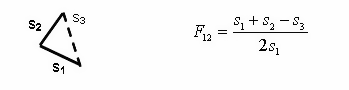
\includegraphics{media/image1059.png}
\caption{WindowHB\_1}
\end{figure}

For~ \emph{n} = 4~ we have:

\begin{figure}[htbp]
\centering
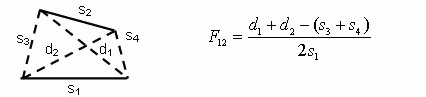
\includegraphics{media/image1060.png}
\caption{WindowHB\_2}
\end{figure}

Applying these to the slat cell shown in Figure~\ref{fig:slat-cell-showing-geometry-for-calculation-of} we have the following:

\begin{equation}
{F_{12}} = \frac{{{d_1} + {d_2} - 2s}}{{2h}}
\end{equation}

\begin{equation}
{F_{13}} = \frac{{h + {s_3} - {d_3}}}{{2h}}{\rm{ ,  etc}}{\rm{.}}
\end{equation}

\begin{figure}[hbtp] % fig 81
\centering
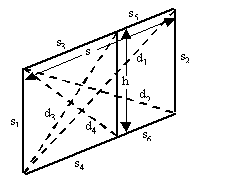
\includegraphics[width=0.9\textwidth, height=0.9\textheight, keepaspectratio=true]{media/image1063.png}
\caption{Slat cell showing geometry for calculation of view factors between the segments of the cell. \protect \label{fig:slat-cell-showing-geometry-for-calculation-of}}
\end{figure}

The sources for the direct-to-diffuse transmittance calculation are:

\begin{equation}
{Q_1} = {Q_2} = {Q_5} = {Q_6} = 0 \;  (and therefore) {J_1} = {J_2} = 0
\end{equation}

\begin{equation}
\left. 
    \begin{array}{l}
      Q_3 = \tau_{dir,dif} \\
      Q_4 = \rho_{dir,dif}^f 
    \end{array} 
  \right\} 
  \;
  \varphi_b \le \varphi_s + \frac{\pi }{2} 
  \;
  \rm{ (beam hits front of slats)}
\end{equation}

\begin{equation}
\left.
    \begin{array}{l}
      Q_3 = \rho_{dir,dif}^b \\
      Q_4 = \tau_{dir,dif}
    \end{array}
  \right\}
  \;
  \varphi_b > \varphi_s + \frac{\pi }{2}
  \;
  \rm{ (beam hits back of slats)}
\end{equation}

For unit incident direct flux, the front direct-to-diffuse transmittance and reflectance of the blind are:

\begin{equation}
  \begin{array}{l}
    \tau_{bl,f}^{dir,dif} = {G_2} \\
    \rho_{bl,f}^{dir,dif} = {G_1}
  \end{array}
\end{equation}

where

\begin{equation}
  \begin{array}{l}
    G_2 = \sum_{j = 3}^6 J_j F_{j2} \\
    G_1 = \sum_{j = 3}^6 J_j F_{j1} 
  \end{array}
\end{equation}

and \({J_3}\) to \({J_6}\) are given by Eq. .~

The front direct absorptance of the blind is then

\begin{equation}
\alpha_{bl,f}^{dir} = 1 - \tau_{bl,f}^{dir,dif} - \tau_{bl,f}^{dir,dir} - \rho_{bl,f}^{dir,dif}
\end{equation}

The direct-to-diffuse calculations are performed separately for solar and visible slat properties to get the corresponding solar and visible blind properties.

\subsubsection{Dependence on Profile Angle}\label{dependence-on-profile-angle}

The direct-to-direct and direct-to-diffuse blind properties are calculated for direct radiation profile angles (see Figure~\ref{fig:a-side-view-of-a-cell-formed-by-adjacent}) ranging from --90\(^{O}\) to +90\(^{O}\) in 5\(^{O}\) increments. (The ``profile angle'' is the angle of incidence in a plane that is perpendicular to the window \emph{and} perpendicular to the slat direction.) In the time step loop the blind properties for a particular profile angle are obtained by interpolation.

\subsubsection{Dependence on Slat Angle}\label{dependence-on-slat-angle}

All blind properties are calculated for slat angles ranging from --90\(^{O}\) to +90\(^{O}\) in 10\(^{O}\) increments. In the time-step loop the slat angle is determined by the slat-angle control mechanism and then the blind properties at that slat angle are determined by interpolation. Three slat-angle controls are available: (1) slat angle is adjusted to just block beam solar incident on the window; (2) slat angle is determined by a schedule; and (3) slat angle is fixed.

\subsubsection{Diffuse-to-Diffuse Transmittance and Reflectance of Blind}\label{diffuse-to-diffuse-transmittance-and-reflectance-of-blind}

To calculate the diffuse-to-diffuse properties, assuming uniformly distributed incident diffuse radiation, each slat bounding the cell is divided into two segments of equal length (Figure~\ref{fig:slat-cell-showing-arrangement-of-segments}), i.e., \({s_3} = {s_4}\) and \({s_5} = {s_6}\) .~ For front-side properties we have a unit source, \({Q_1} = 1\) .~ All the other \({Q_i}\) are zero. Using this source value, we apply the methodology described above to obtain \emph{G\(_{2}\)}and \emph{G\(_{1}\)}. We then have

\begin{equation}
\begin{array}{l}\tau_{bl,f}^{dif,dif} = {G_2}\\\rho_{bl,f}^{dif,dif} = {G_1}\\\alpha_{bl,f}^{dif} = 1 - \tau_{bl,f}^{dif,dif} - \rho_{bl,f}^{dif,dif}\end{array}
\end{equation}

The back-side properties are calculated in a similar way by setting \emph{Q\(_{2}\)} = 1 with the other \({Q_i}\) equal to zero.

The diffuse-to-diffuse calculations are performed separately for solar, visible and IR slat properties to get the corresponding solar, visible and IR blind properties.

\begin{figure}[hbtp] % fig 82
\centering
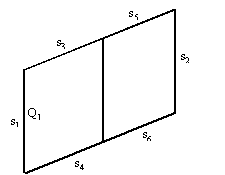
\includegraphics[width=0.9\textwidth, height=0.9\textheight, keepaspectratio=true]{media/image1078.png}
\caption{Slat cell showing arrangement of segments and location of source for calculation of diffuse-to-diffuse optical properties. \protect \label{fig:slat-cell-showing-arrangement-of-segments}}
\end{figure}

\subsubsection{Blind properties for sky and ground diffuse radiation}\label{blind-properties-for-sky-and-ground-diffuse-radiation}

For horizontal slats on a vertical window (the most common configuration) the blind diffuse-to-diffuse properties will be sensitve to whether the radiation is incident upward from the ground or downward from the sky (Figure~\ref{fig:side-view-of-horizontal-slats-in-a-vertical}). For this reason we also calculate the following solar properties for a blind consisting of horizontal slats in a vertical plane:

\(\tau_{bl,f}^{gnd - dif,dif} = {\rm{ }}\) front transmittance for ground diffuse solar

\(\tau_{bl,f}^{sky - dif,dif} = {\rm{ }}\) front transmittance for sky diffuse solar

$\rho_{bl,f}^{gnd - dif,dif} = $ front reflectance for ground diffuse solar

\(\rho_{bl,f}^{sky - dif,dif} = {\rm{ }}\) front reflectance for sky diffuse solar

\(\alpha_{bl,f}^{gnd - dif,dif} = {\rm{ }}\) front absorptance for ground diffuse solar

\(\alpha_{bl,f}^{sky - dif,dif} = {\rm{ }}\) front absorptance for sky diffuse solar

These are obtained by integrating over sky and ground elements, as shown in Figure~\ref{fig:side-view-of-horizontal-slats-in-a-vertical}, treating each element as a source of direct radiation of irradiance \(I({\phi_s})\) ~incident on the blind at profile angle \({\phi_s}\) . This gives:

\begin{equation}
\tau_{bl,f}^{sky - dif,dif} = \frac{{\int\limits_0^{\pi /2} {\left[ {\tau_{bl,f}^{dir,dir}({\phi_s}) + \tau_{bl,f}^{dir,dif}({\phi_s})} \right]{I_{sky}}({\phi_s})\cos {\phi_s}d{\phi_s}} }}{{\int\limits_0^{\pi /2} {{I_{sky}}({\phi_s})\cos {\phi_s}d{\phi_s}} }}
\end{equation}

\begin{equation}
\rho_{bl,f}^{sky - dif,dif} = \frac{{\int\limits_0^{\pi /2} {\rho_{bl,f}^{dir,dif}{I_{sky}}({\phi_s})\cos {\phi_s}d{\phi_s}} }}{{\int\limits_0^{\pi /2} {{I_{sky}}({\phi_s})\cos {\phi_s}d{\phi_s}} }}
\end{equation}

\begin{equation}
\alpha_{bl,f}^{sky - dif} = \frac{{\int\limits_0^{\pi /2} {\alpha_{bl,f}^{dir}{I_{sky}}({\phi_s})\cos {\phi_s}d{\phi_s}} }}{{\int\limits_0^{\pi /2} {{I_{sky}}({\phi_s})\cos {\phi_s}d{\phi_s}} }}
\end{equation}

\begin{figure}[hbtp] % fig 83
\centering
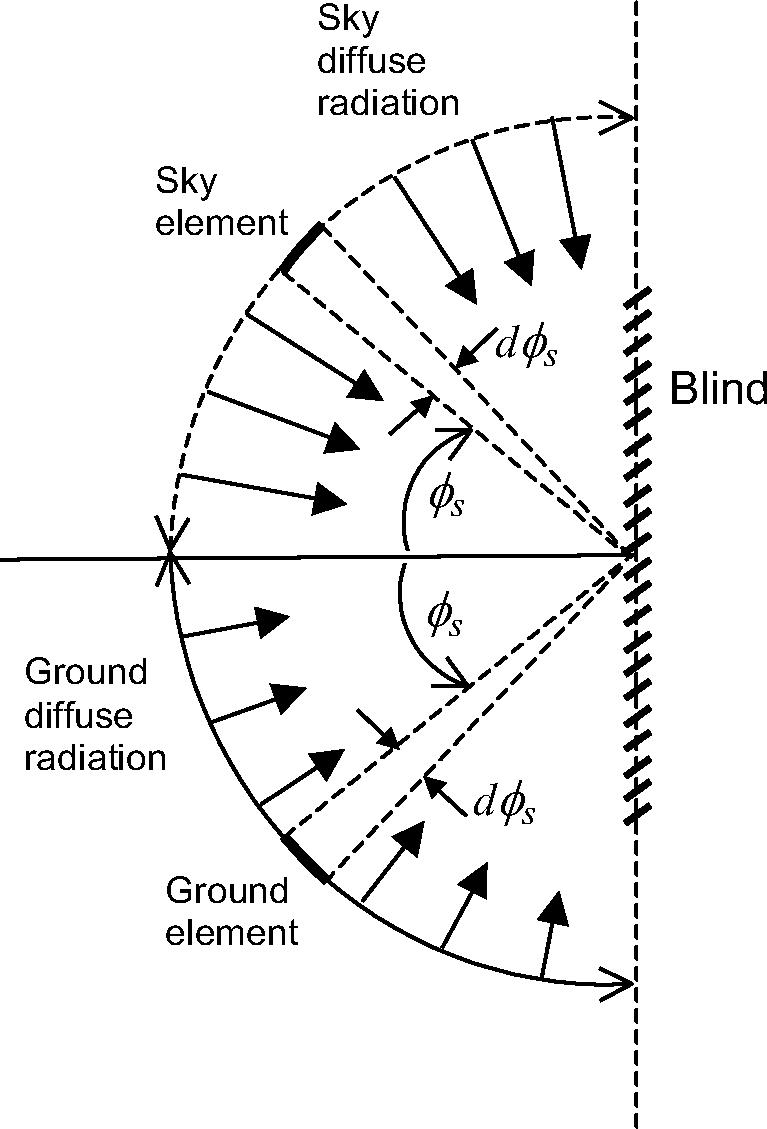
\includegraphics[width=0.9\textwidth, height=0.9\textheight, keepaspectratio=true]{media/image1090.png}
\caption{Side view of horizontal slats in a vertical blind showing geometry for calculating blind transmission, reflection and absorption properties for sky and ground diffuse radiation. \protect \label{fig:side-view-of-horizontal-slats-in-a-vertical}}
\end{figure}

We assume that the sky radiance is uniform. This means that \({I_{sky}}\) is independent of \({\phi_s}\) , giving:

\begin{equation}
\tau_{bl,f}^{sky - dif,dif} = \int\limits_0^{\pi /2} {\left[ {\tau_{bl,f}^{dir,dir} + \tau_{bl,f}^{dir,dif}} \right]\cos {\phi_s}d{\phi_s}}
\end{equation}

\begin{equation}
\rho_{bl,f}^{sky - dif,dif} = \int\limits_0^{\pi /2} {\rho_{bl,f}^{dir,dif}\cos {\phi_s}d{\phi_s}}
\end{equation}

\begin{equation}
\alpha_{bl,f}^{sky - dif} = \int\limits_0^{\pi /2} {\alpha_{bl,f}^{dir}\cos {\phi_s}d{\phi_s}}
\end{equation}

The corresponding ground diffuse quantities are obtained by integrating \({\phi_s}\) ~from \(- \pi /2\) ~to 0.

An improvement to this calculation would be to allow the sky radiance distribution to be non-uniform, i.e.,~ to depend on sun position and sky conditions, as is done in the detailed daylighting calculation (see ``Sky Luminance Distributions'' under ``Daylight Factor Calculation'').

\subsubsection{Correction Factor for Slat Thickness}\label{correction-factor-for-slat-thickness}

A correction has to be made to the blind transmittance, reflectance and absorptance properties to account for the amount of radiation incident on a blind that is reflected and absorbed by the slat edges (the slats are assumed to be opaque to radiation striking the slat edges). This is illustrated in Figure~\ref{fig:side-view-of-slats-showing-geometry-for} for the case of direct radiation incident on the blind. The slat cross-section is assumed to be rectangular. The quantity of interest is the fraction, \emph{f\(_{edge}\)}, of direct radiation incident on the blind that strikes the slat edges. Based on the geometry shown in Figure~\ref{fig:side-view-of-slats-showing-geometry-for} we see that

\begin{equation}
{f_{edge}} = \frac{{t\cos \gamma }}{{\left( {h + \frac{t}{{\cos \xi }}} \right)\cos {\varphi_s}}} = \frac{{t\cos ({\varphi_s} - \xi )}}{{\left( {h + \frac{t}{{\cos \xi }}} \right)\cos {\varphi_s}}} = \frac{{t\sin ({\varphi_b} - {\varphi_s})}}{{\left( {h + \frac{t}{{\sin {\varphi_b}}}} \right)\cos {\varphi_s}}}
\end{equation}

The edge correction factor for diffuse incident radiation is calculated by averaging this value of \emph{f\(_{edge}\)} over profile angles, \emph{φ\(_{s}\)}, from --90\(^{O}\) to +90\(^{O}\).

As an example of how the edge correction factor is applied, the following two equations show how blind front diffuse transmittance and reflectance calculated assuming zero slat thickness are modified by the edge correction factor. It is assumed that the edge transmittance is zero and that the edge reflectance is the same as the slat front reflectance, \emph{ρ\(_{f}\)}.

\begin{equation}
\begin{array}{l}\tau_{bl,f}^{dif,dif} \to \tau_{bl,f}^{dif,dif}\left( {1 - {f_{edge}}} \right)\\\rho_{bl,f}^{dif} \to \rho_{bl,f}^{dif}\left( {1 - {f_{edge}}} \right) + {f_{edge}}{\rho_f}\end{array}
\end{equation}

\begin{figure}[hbtp] % fig 84
\centering
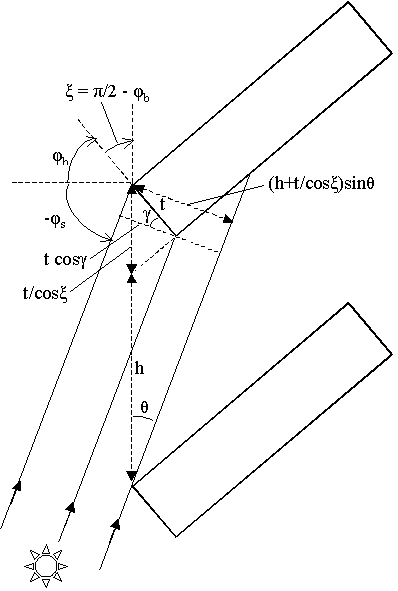
\includegraphics[width=0.9\textwidth, height=0.9\textheight, keepaspectratio=true]{media/image1100.png}
\caption{Side view of slats showing geometry for calculation of slat edge correction factor for incident direct radiation. \protect \label{fig:side-view-of-slats-showing-geometry-for}}
\end{figure}

\subsubsection{Comparison with ISO 15099 Calculation of Blind Optical Properties}\label{comparison-with-iso-15099-calculation-of-blind-optical-properties}

Table~\ref{table:comparison-of-blind-optical-properties} compares EnergyPlus and ISO 15099 {[}2001{]} calculations of blind optical properties for a variety of profile angles, slat angles and slat optical properties. The ISO 15099 calculation method is similar to that used in EnergyPlus, except that the slats are divided into five equal segments. The ISO 15099 and EnergyPlus results agree to within 12\%, except for the solar transmittances for the 10-degree slat angle case. Here the transmittances are small (from 1\% to about 5\%) but differ by about a factor of up to two between ISO 15099 and EnergyPlus. This indicates that the slats should be divided into more than two segments at small slat angles.

% table 33
\begin{longtable}[c]{p{1.0in}p{0.4in}p{0.4in}p{0.4in}p{0.4in}p{0.4in}p{0.4in}p{0.4in}p{0.4in}p{0.4in}p{0.4in}}
\caption{Comparison of blind optical properties calculated with the EnergyPlus and ISO 15099 methods. EnergyPlus values that differ by more than 12\% from ISO 15099 values are shown in bold italics. \label{table:comparison-of-blind-optical-properties}} \tabularnewline
\toprule 
\multicolumn{11}{l}{\textbf{Slat Properties}} \tabularnewline
\midrule
\endfirsthead

\caption[]{Comparison of blind optical properties calculated with the EnergyPlus and ISO 15099 methods. EnergyPlus values that differ by more than 12\% from ISO 15099 values are shown in bold italics.} \tabularnewline
\toprule 
\multicolumn{11}{l}{\textbf{Slat Properties}} \tabularnewline
\midrule
\endhead

Separation (m) & \multicolumn{2}{c}{0.012} & \multicolumn{2}{c}{0.012} & \multicolumn{2}{c}{0.012} & \multicolumn{2}{c}{0.012} & \multicolumn{2}{c}{0.012} \tabularnewline
Width (m) & \multicolumn{2}{c}{0.016} & \multicolumn{2}{c}{0.016} & \multicolumn{2}{c}{0.016} & \multicolumn{2}{c}{0.016} & \multicolumn{2}{c}{0.016} \tabularnewline
Angle (deg) & \multicolumn{2}{c}{45} & \multicolumn{2}{c}{45} & \multicolumn{2}{c}{45} & \multicolumn{2}{c}{10} & \multicolumn{2}{c}{45} \tabularnewline
IR transmittance & \multicolumn{2}{c}{0} & \multicolumn{2}{c}{0} & \multicolumn{2}{c}{0} & \multicolumn{2}{c}{0} & \multicolumn{2}{c}{0.4} \tabularnewline
IR emissivity, front side & \multicolumn{2}{c}{0.9} & \multicolumn{2}{c}{0.9} & \multicolumn{2}{c}{0.9} & \multicolumn{2}{c}{0.9} & \multicolumn{2}{c}{0.55} \tabularnewline
IR emissivity, back side & \multicolumn{2}{c}{0.9} & \multicolumn{2}{c}{0.9} & \multicolumn{2}{c}{0.9} & \multicolumn{2}{c}{0.9} & \multicolumn{2}{c}{0.55} \tabularnewline
Solar transmittance & \multicolumn{2}{c}{0} & \multicolumn{2}{c}{0} & \multicolumn{2}{c}{0} & \multicolumn{2}{c}{0} & \multicolumn{2}{c}{0.4} \tabularnewline
Solar reflectance, front side & \multicolumn{2}{c}{0.7} & \multicolumn{2}{c}{0.55} & \multicolumn{2}{c}{0.7} & \multicolumn{2}{c}{0.7} & \multicolumn{2}{c}{0.5} \tabularnewline
Solar reflectance, back side & \multicolumn{2}{c}{0.7} & \multicolumn{2}{c}{0.55} & \multicolumn{2}{c}{0.4} & \multicolumn{2}{c}{0.4} & \multicolumn{2}{c}{0.5} \tabularnewline \midrule
 \tabularnewline \midrule
Solar Profile angle (deg) & 0 & 60 & 0 & 60 & 0 & 60 & 0 & 60 & 0 & 60 \tabularnewline \midrule
 \tabularnewline \midrule
\multicolumn{11}{l}{\textbf{Calculated blind properties} (first row = ISO 15099 calculation,} \tabularnewline
\multicolumn{11}{l}{second row (in italics) = EnergyPlus calculation)} \tabularnewline \midrule
Front solar transmittance, direct to Direct & 0.057 \quad \quad \textit{0.057} & 0 \quad \quad \textit{0} & 0.057 \quad \quad \textit{0.057} & 0 \quad \quad \textit{0} & 0.057 \quad \quad \textit{0.057} & 0 \quad \quad \textit{0} & 0 \quad \quad \textit{0} & 0 \quad \quad \textit{0} & 0.057 \quad \quad \textit{0.057} & 0 \quad \quad \textit{0} \tabularnewline
Back solar transmittance, direct to direct & 0.057 \quad \quad \textit{0.057} & 0.310 \quad \quad \textit{0.309} & 0.057 \quad \quad \textit{0.057} & 0.310 \quad \quad \textit{0.309} & 0.057 \quad \quad \textit{0.057} & 0.310 \quad \quad \textit{0.309} & 0 \quad \quad \textit{0} & 0.088 \quad \quad \textit{0.087} & 0.057 \quad \quad \textit{0.057} & 0.310 \quad \quad \textit{0.309} \tabularnewline
Front solar transmittance, direct to diffuse & 0.141 \quad \quad \textit{0.155} & 0.073 \quad \quad \textit{0.074} & 0.090 \quad \quad \textit{0.100} & 0.047 \quad \quad \textit{0.048} & 0.096 \quad \quad \textit{0.104} & 0.051 \quad \quad \textit{0.051} & 0.012 \quad \quad \textbf{\textit{0.019}} & 0.005 \quad \quad \textbf{\textit{0.006}} & 0.373 \quad \quad \textit{0.375} & 0.277 \quad \quad \textit{0.275} \tabularnewline
Back solar transmittance, direct to diffuse & 0.141 \quad \quad \textit{0.155} & 0.288 \quad \quad \textit{0.284} & 0.090 \quad \quad \textit{0.100} & 0.216 \quad \quad \textit{0.214} & 0.076 \quad \quad \textit{0.085} & 0.271 \quad \quad \textit{0.269} & 0.011 \quad \quad \textbf{\textit{0.019}} & 0.027 \quad \quad \textbf{\textit{0.052}} & 0.373 \quad \quad \textit{0.375} & 0.306 \quad \quad \textit{0.304} \tabularnewline
Front solar reflectance, direct to diffuse & 0.394 \quad \quad \textit{0.389} & 0.558 \quad \quad \textit{0.558} & 0.295 \quad \quad \textit{0.293} & 0.430 \quad \quad \textit{0.431} & 0.371 \quad \quad \textit{0.368} & 0.544 \quad \quad \textit{0.546} & 0.622 \quad \quad \textit{0.636} & 0.678 \quad \quad \textit{0.679} & 0.418 \quad \quad \textit{0.416} & 0.567 \quad \quad \textit{0.568} \tabularnewline
Back solar reflectance, direct to diffuse & 0.394 \quad \quad \textit{0.389} & 0.103 \quad \quad \textit{0.115} & 0.295 \quad \quad \textit{0.293} & 0.066 \quad \quad \textit{0.074} & 0.216 \quad \quad \textit{0.214} & 0.070 \quad \quad \textit{0.077} & 0.356 \quad \quad \textit{0.363} & 0.273 \quad \quad \textit{0.272} & 0.418 \quad \quad \textit{0.416} & 0.273 \quad \quad \textit{0.275} \tabularnewline
Front solar transmittance, hemispherical diffuse to diffuse & 0.332 \quad \quad \textit{0.338} &  & 0.294 \quad \quad \textit{0.298} &  & 0.291 \quad \quad \textit{0.295} &  & 0.038 \quad \quad \textbf{\textit{0.053}} &  & 0.495 \quad \quad \textit{0.502} \tabularnewline
Back solar transmittance, hemispherical diffuse to diffuse & 0.332 \quad \quad \textit{0.338} &  & 0.294 \quad \quad \textit{0.298} &  & 0.291 \quad \quad \textit{0.295} &  & 0.038 \quad \quad \textbf{\textit{0.053}} &  & 0.495 \quad \quad \textit{0.502} &  \tabularnewline
Front hemispherical IR transmittance & 0.227 \quad \quad \textit{0.227} &  & 0.227 \quad \quad \textit{0.227} &  & 0.227 \quad \quad \textit{0.227} &  & 0.0245 \quad \quad \textit{0.025} &  & 0.385 \quad \quad \textit{0.387} &  \tabularnewline
Back hemispherical IR transmittance & 0.227 \quad \quad \textit{0.227} &  & 0.227 \quad \quad \textit{0.227} &  & 0.227 \quad \quad \textit{0.227} &  & 0.0245 \quad \quad \textit{0.025} &  & 0.385 \quad \quad \textit{0.387} &  \tabularnewline
Front hemispherical IR emissivity & 0.729 \quad \quad \textit{0.730} &  & 0.729 \quad \quad \textit{0.730} &  & 0.729 \quad \quad \textit{0.730} &  & 0.890 \quad \quad \textit{0.895} &  & 0.536 \quad \quad \textit{0.534} &  \tabularnewline
Back hemispherical IR emissivity & 0.729 \quad \quad \textit{0.730} &  & 0.729 \quad \quad \textit{0.730} &  & 0.729 \quad \quad \textit{0.730} &  & 0.890 \quad \quad \textit{0.895} &  & 0.536 \quad \quad \textit{0.534} &  \tabularnewline
\bottomrule
\end{longtable}

\subsubsection{Blind/Glazing System Properties for Short-Wave Radiation}\label{blindglazing-system-properties-for-short-wave-radiation}

When a blind is in place we have the following expressions for the system transmittance, the system glass layer absorptance, and the system blind absorptance, taking inter-reflection between blind and glazing into account. The system properties, indicated by ``sys,'' are given in terms of the isolated blind properties (i.e., blind properties in the absence of the glazing)---indicated by ``bl'' ---and the isolated glazing properties (i.e., glazing properties in the absence of the blind)---indicated by ``gl.''

\subsubsection{Interior Blind}\label{interior-blind}

The system properties when an interior blind is in place are the following:

\begin{equation}
T_{f,sys}^{dir,all}(\phi ,{\phi_s}) = T_{gl}^{dir}(\phi )\left( {\tau_{bl,f}^{dir,dir}({\phi_s}) + \tau_{bl,f}^{dir,dif}({\phi_s}) + \frac{{\tau_{bl,f}^{dif}\rho_{bl,f}^{dir,dif}({\phi_s})R_{gl,b}^{dif}}}{{1 - \rho_{bl,f}^{dif}R_{gl,b}^{dif}}}} \right)
\end{equation}

\begin{equation}
A_{gl,j,f}^{dir,sys}(\phi ,{\phi_s}) = A_{gl,j,f}^{dir}(\phi ) + \frac{{T_{gl}^{dir}(\phi )\alpha_{gl,j,b}^{dif}\rho_{bl,f}^{dir}({\phi_s})}}{{1 - \rho_{bl,f}^{dir}({\phi_s})R_{gl,b}^{dif}}}{\rm{,    }}j = 1,N
\end{equation}

\begin{equation}
\alpha_{bl,f}^{dir,sys}(\phi ,{\phi_s}) = T_{gl}^{dir}(\phi )\left( {\alpha_{bl,f}^{dir}({\phi_s}) + \frac{{\rho_{bl,f}^{dir}({\phi_s})R_{gl,b}^{dif}\alpha_{bl,f}^{dif}}}{{1 - \rho_{bl,f}^{dif}R_{gl,b}^{dif}}}} \right)
\end{equation}

\begin{equation}
T_{f,sys}^{dif,dif} = \frac{{T_{gl}^{dif}\tau_{bl,f}^{dif,dif}}}{{1 - \rho_{bl,f}^{dif}R_{gl,b}^{dif}}}
\end{equation}

\begin{equation}
T_{f,sys}^{sky - dif,dif} = \frac{{T_{gl}^{dif}\tau_{bl,f}^{sky - dif,dif}}}{{1 - \rho_{bl,f}^{sky - dif}R_{gl,b}^{dif}}}
\end{equation}

\begin{equation}
T_{f,sys}^{gnd - dif,dif} = \frac{{T_{gl}^{dif}\tau_{bl,f}^{gnd - dif,dif}}}{{1 - \rho_{bl,f}^{gnd - dif}R_{gl,b}^{dif}}}
\end{equation}

\begin{equation}
A_{gl,j,f}^{dif,sys} = A_{gl,j,f}^{dif} + \frac{{T_{gl}^{dif}\rho_{bl,f}^{dif}A_{gl,j,b}^{dif}}}{{1 - \rho_{bl,f}^{dif}R_{gl,b}^{dif}}}{\rm{,    }}j = 1,N
\end{equation}

\begin{equation}
A_{gl,j,f}^{sky - dif,sys} = A_{gl,j,f}^{dif} + \frac{{T_{gl}^{dif}\rho_{bl,f}^{sky - dif}A_{gl,j,b}^{dif}}}{{1 - \rho_{bl,f}^{sky - dif}R_{gl,b}^{dif}}}{\rm{,    }}j = 1,N
\end{equation}

\begin{equation}
A_{gl,j,f}^{gnd - dif,sys} = A_{gl,j,f}^{dif} + \frac{{T_{gl}^{dif}\rho_{bl,f}^{gnd - dif}A_{gl,j,b}^{dif}}}{{1 - \rho_{bl,f}^{gnd - dif}R_{gl,b}^{dif}}}{\rm{,    }}j = 1,N
\end{equation}

\begin{equation}
\alpha_{bl,f}^{dif,sys} = \frac{{T_{gl}^{dif}\alpha_{bl,f}^{dif}}}{{1 - \rho_{bl,f}^{dif}R_{gl,b}^{dif}}}
\end{equation}

\begin{equation}
\alpha_{bl,f}^{sky - dif,sys} = \frac{{T_{gl}^{dif}\alpha_{bl,f}^{sky - dif}}}{{1 - \rho_{bl,f}^{sky - dif}R_{gl,b}^{dif}}}
\end{equation}

\begin{equation}
\alpha_{bl,f}^{gnd - dif,sys} = \frac{{T_{gl}^{dif}\alpha_{bl,f}^{gnd - dif}}}{{1 - \rho_{bl,f}^{gnd - dif}R_{gl,b}^{dif}}}
\end{equation}

\subsubsection{Exterior Blind}\label{exterior-blind}

The system properties when an exterior blind is in place are the following:

\begin{equation}
T_{f,sys}^{dir,all}(\phi ,{\phi_s}) = \tau_{bl,f}^{dir,dir}({\phi_s})\left( {T_{gl}^{dir}(\phi ) + \frac{{T_{gl}^{dif}R_{gl,f}^{dir}\rho_{bl,b}^{dir,dif}}}{{1 - R_{gl,f}^{dif}\rho_{bl,b}^{dif}}}} \right) + \frac{{\tau_{bl}^{dir,dif}({\phi_s})T_{gl}^{dif}}}{{1 - R_{gl,f}^{dif}\rho_{bl,b}^{dif}}}
\end{equation}

\begin{equation}
A_{gl,j,f}^{dir,sys}(\phi ,\phi_s) = 
     \tau_{bl,f}^{dir,dir}(\phi_s) A_{gl,j,f}^{dir}(\phi ) + 
     \frac{
       \left(
         \tau_{bl,f}^{dir,dir}(\phi_s) R_{gl}^{dir}(\phi) \rho_{bl,b}^{dir}(\phi_s)+ \tau_{bl,f}^{dir,dif}(\phi_s)
       \right) A_{gl,j,f}^{dif}
     } {
       1 - R_{gl,f}^{dif}\rho_{bl,b}^{dif}
     },\;j = 1,N
\end{equation}

\begin{equation}
\begin{split}
\alpha_{bl,f}^{dir,sys}(\phi ,\phi_s) =& \alpha_{bl,f}^{dir}(\phi_s) + \alpha_{bl,b}^{dir}(\phi_s) R_{gl,f}^{dir}(\phi) \tau_{bl,f}^{dir,dir}(\phi_s) \\
&+ \frac{\alpha_{bl,b}^{dif}R_{gl,f}^{dif}}{1 - \rho_{bl,b}^{dif} R_{gl,f}^{dif}}\left(R_{gl,f}^{dir}(\phi) \tau_{bl,f}^{dir,dir}(\phi_s) \rho_{bl,b}^{dir}(\phi_s) + \tau_{bl,f}^{dir,dif}(\phi_s) \right)
\end{split}
\end{equation}

\begin{equation}
T_{f,sys}^{dif,dif} = \frac{{\tau_{bl,f}^{dif,dif}T_{gl}^{dif}}}{{1 - R_{gl,f}^{dif}\rho_{bl,b}^{dif}}}
\end{equation}

\begin{equation}
T_{f,sys}^{sky - dif,dif} = \frac{{\tau_{bl,f}^{sky - dif,dif}T_{gl}^{dif}}}{{1 - R_{gl,f}^{dif}\rho_{bl,b}^{dif}}}
\end{equation}

\begin{equation}
T_{f,sys}^{gnd - dif,dif} = \frac{{\tau_{bl,f}^{gnd - dif,dif}T_{gl}^{dif}}}{{1 - R_{gl,f}^{dif}\rho_{bl,b}^{dif}}}
\end{equation}

\begin{equation}
A_{gl,j,f}^{dif,sys} = \frac{{\tau_{bl,f}^{dif,dif}A_{gl,j,f}^{dif}}}{{1 - R_{gl,f}^{dif}\rho_{bl,b}^{dif}}},{\rm{    }}j = 1,N
\end{equation}

\begin{equation}
A_{gl,j,f}^{sky - dif,sys} = \frac{{\tau_{bl,f}^{sky - dif,dif}A_{gl,j,f}^{dif}}}{{1 - R_{gl,f}^{dif}\rho_{bl,b}^{dif}}},{\rm{    }}j = 1,N
\end{equation}

\begin{equation}
A_{gl,j,f}^{gnd - dif,sys} = \frac{{\tau_{bl,f}^{gnd - dif,dif}A_{gl,j,f}^{dif}}}{{1 - R_{gl,f}^{dif}\rho_{bl,b}^{dif}}},{\rm{    }}j = 1,N
\end{equation}

\begin{equation}
\alpha_{bl,f}^{dif,sys} = \alpha_{bl,f}^{dif} + \frac{{\tau_{bl,f}^{dif,dif}R_{gl,f}^{dif}}}{{1 - R_{gl,f}^{dif}\rho_{bl,b}^{dif}}}\alpha_{bl,b}^{dif}
\end{equation}

\begin{equation}
\alpha_{bl,f}^{sky - dif,sys} = \alpha_{bl,f}^{sky - dif} + \frac{{\tau_{bl,f}^{sky - dif,dif}R_{gl,f}^{dif}}}{{1 - R_{gl,f}^{dif}\rho_{bl,b}^{dif}}}\alpha_{bl,b}^{dif}
\end{equation}

\begin{equation}
\alpha_{bl,f}^{gnd - dif,sys} = \alpha_{bl,f}^{gnd - dif} + \frac{{\tau_{bl,f}^{gnd - dif,dif}R_{gl,f}^{dif}}}{{1 - R_{gl,f}^{dif}\rho_{bl,b}^{dif}}}\alpha_{bl,b}^{dif}
\end{equation}

\subsubsection{Blind/Glazing System Properties for Long-Wave Radiation}\label{blindglazing-system-properties-for-long-wave-radiation}

The program calculates how much long-wave radiation is absorbed by the blind and by the adjacent glass surface. The effective emissivity (long-wave absorptance) of an interior or exterior blind, taking into account reflection of long-wave radiation between the glass and blind, is given by

\begin{equation}
\varepsilon_{bl}^{lw,eff} = \varepsilon_{bl}^{lw}\left( {1 + \frac{{\tau_{bl}^{lw}\rho_{gl}^{lw}}}{{1 - \rho_{bl}^{lw}\rho_{gl}^{lw}}}} \right)
\end{equation}

where \(\rho_{gl}^{lw}\) is the long-wave reflectance of the outermost glass surface for an exterior blind or the innermost glass surface for an interior blind, and it is assumed that the long-wave transmittance of the glass is zero.

The effective innermost (for interior blind) or outermost (for exterior blind) glass surface emissivity when the blind is present is

\begin{equation}
\varepsilon_{gl}^{lw,eff} = \varepsilon_{gl}^{lw}\frac{{\tau_{bl}^{lw}}}{{1 - \rho_{bl}^{lw}\rho_{gl}^{lw}}}
\end{equation}

The effective inside surface emissivity is the sum of the effective blind and effective glass emissivities:

\begin{equation}
\varepsilon_{ins}^{lw,eff} = \varepsilon_{bl}^{lw,eff} + \varepsilon_{gl}^{lw,eff}
\end{equation}

The effective temperature of the blind/glazing combination that is used to calculate the window's contribution to the zone's mean radiant temperature (MRT) is given by

\begin{equation}
T_{}^{eff} = \frac{{\varepsilon_{bl}^{lw,eff}{T_{bl}} + \varepsilon_{gl}^{lw,eff}{T_{gl}}}}{{\varepsilon_{bl}^{lw,eff} + \varepsilon_{gl}^{lw,eff}}}
\end{equation}

\subsubsection{Solar Radiation Transmitted and Absorbed by a Window/Blind System}\label{solar-radiation-transmitted-and-absorbed-by-a-windowblind-system}

Let the direct solar incident on the window be

\begin{equation}
{I_{dir,inc}} = {f_{sunlit}}{I_{dir,norm}}\cos \phi {\rm{    }}(W/{m^2})
\end{equation}

where \({f_{sunlit}}\) is the fraction of the window that is sunlit (determined by the shadowing calculations), \({I_{dir,norm}}\) is the direct normal solar irradiance, and \(\phi\) ~is the angle of incidence.

Let \({I_{sky,inc}}\) be the irradiance on the window due to diffuse solar radiation from the sky (W/m\(^{2}\)) and let \({I_{gnd,inc}}\) be the irradiance on the window due to diffuse solar radiation from the ground (W/m\(^{2}\)).

Then we have the following expressions for different classes of transmitted and absorbed solar radiation for the window/blind system (where \({\phi_s}\) is the direct solar profile angle), all in W/m\(^{2}\):

\emph{Direct solar entering zone from incident direct solar:}

\begin{equation}
{I_{dir,inc}}T_{f,sys}^{dir,dir}(\phi ,{\phi_s})
\end{equation}

\emph{Diffuse solar entering zone from incident direct solar:}

\begin{equation}
{I_{dir,inc}}T_{f,sys}^{dir,dif}(\phi ,{\phi_s})
\end{equation}

\emph{Direct solar absorbed by blind:}

\begin{equation}
{I_{dir,inc}}\alpha_{bl,f}^{dir,sys}(\phi ,{\phi_s})
\end{equation}

\emph{Direct solar absorbed by glass layers:}

\begin{equation}
{I_{dir,inc}}A_{gl,j,f}^{dir,sys}(\phi ,{\phi_s}),{\rm{    }}j = 1,N
\end{equation}

\subsubsection{For windows whose blinds have vertical slats:}\label{for-windows-whose-blinds-have-vertical-slats}

\emph{Diffuse solar entering zone from incident diffuse solar:}

\begin{equation}
({I_{sky,inc}} + {I_{gnd,inc}})T_{f,sys}^{dif,dif}
\end{equation}

\emph{Diffuse solar absorbed by blind:}

\begin{equation}
({I_{sky,inc}} + {I_{gnd,inc}})\alpha_{bl,f}^{dif,sys}
\end{equation}

\emph{Diffuse solar absorbed by glass layers:}

\begin{equation}
({I_{sky,inc}} + {I_{gnd,inc}})A_{gl,j,f}^{dif,sys},{\rm{   }}j = 1,N{\rm{ }}
\end{equation}

\subsubsection{\texorpdfstring{For windows of tilt angle \(\gamma\) ~whose blinds have horizontal slats:}{For windows of tilt angle \textbackslash{}gamma ~whose blinds have horizontal slats:}}\label{for-windows-of-tilt-angle-gamma-whose-blinds-have-horizontal-slats}

(vertical windows have tilt = 90\(^{O}\), horizontal windows have tilt = 0\(^{O}\))

\emph{Diffuse solar entering zone from incident diffuse solar:}

\begin{equation}
\begin{split}
T_{f,sys}^{sky - dif,dif}\left[ {\left( {1 - \frac{{|\cos \gamma |}}{2}} \right){I_{sky,inc}} + \frac{{|\cos \gamma |}}{2}{I_{gnd,inc}}} \right] + \\
T_{f,sys}^{gnd - dif,dif}\left[ {\frac{{|\cos \gamma |}}{2}{I_{sky,inc}} + \left( {1 - \frac{{|\cos \gamma |}}{2}} \right){I_{gnd,inc}}} \right]
\end{split}
\end{equation}

\emph{Diffuse solar absorbed by blind:}

\begin{equation}
\begin{split}
\alpha_{bl,f}^{sky - dif,sys}\left[ {\left( {1 - \frac{{|\cos \gamma |}}{2}} \right){I_{sky,inc}} + \frac{{|\cos \gamma |}}{2}{I_{gnd,inc}}} \right] + \\
\alpha_{bl,f}^{gnd - dif,sys}\left[ {\frac{{|\cos \gamma |}}{2}{I_{sky,inc}} + \left( {1 - \frac{{|\cos \gamma |}}{2}} \right){I_{gnd,inc}}} \right]
\end{split}
\end{equation}

\emph{Diffuse solar absorbed by glass layers:}

\begin{equation}
\begin{array}{l}A_{gl,j,f}^{sky - dif,sys}\left[ {\left( {1 - \frac{{|\cos \gamma |}}{2}} \right){I_{sky,inc}} + \frac{{|\cos \gamma |}}{2}{I_{gnd,inc}}} \right] + \\A_{gl,j,f}^{gnd - dif,sys}\left[ {\frac{{|\cos \gamma |}}{2}{I_{sky,inc}} + \left( {1 - \frac{{|\cos \gamma |}}{2}} \right){I_{gnd,inc}}} \right],{\rm{    }}j = 1,N\end{array}
\end{equation}

\subsubsection{Screens}\label{screens}

The model for window screens currently allows placement on the exterior surface of a window system (i.e., between glass and interior window screens can not be modeled). The exterior screen is modeled as a planar semi-transparent sheet having specular transmittance that is dependent on the angle of incidence of beam solar radiation. The screen transmittance algorithm includes two components. The first one, \emph{T\(_{beam}\)} (α', φ'), accounts for the blockage of the sun's rays by the screen material. This component accounts for the beam solar radiation passing through the screen openings without hitting the screen material. The second part, \emph{T\(_{scatt}\)}~ (α', φ'), accounts for the additional flux of transmitted beam solar radiation by diffuse reflectance (scattering) from the screen material. Since the reflected component is small compared with the incident beam and the direction of scattering is highly dependent on incident angle, the component of transmitted beam radiation due to screen material reflectance can be treated in one of three ways based on a user input to the model.

The user may elect not to model the inward reflected beam transmittance due to the uncertainty of the direction of scattering or its low magnitude for low-reflecting screen materials. The user may alternately choose to model the inwardly-reflected transmitted beam as an additive component to the direct beam transmittance in the same solid angle and direction. Finally, the additional flux due to the inward reflection of direct beam radiation may be modeled as hemispherically-diffuse transmittance.

This reflected beam transmittance component depends upon the diffuse (i.e., beam-to-diffuse) reflectance of the screen material, so this reflectance (ρ\(_{sc}\)) is a required input to the model. Guidance input values for this diffuse reflectance are provided, to account for screens that are dark, medium, or light colored in appearance, in the likely case that more accurate values for the material reflectance are difficult or time-consuming to obtain. If the diffuse reflectance of the screen material is known, use this value in place of the guidance provided.

The model is based on an orthogonal crossed cylinder geometry in which the screen material's cylindrical diameter and spacing are known. The model assumes that the screen material diameter and spacing are the same in both directions. Figure~\ref{fig:screen-model-rendering-of-intersecting} shows a rendering of intersecting orthogonal crossed cylinders used as the basis for the EnergyPlus screen model.

\begin{figure}[hbtp] % fig 85
\centering
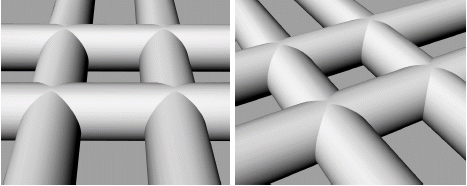
\includegraphics[width=0.9\textwidth, height=0.9\textheight, keepaspectratio=true]{media/image1148.png}
\caption{Screen model rendering of intersecting orthogonal crossed cylinders \protect \label{fig:screen-model-rendering-of-intersecting}}
\end{figure}

If the required screen material dimensions are not available from the manufacturer, they may be determined using the following procedure:

\begin{itemize}
\item
  Lay the screen next to a finely-divided scale or ruler. A magnifying glass may be helpful in determining the screen material dimensions. Alternately, a photograph can be taken and the image enlarged.
\item
  Determine the diameter \emph{D} of an individual screen material ``cylinder''. Average the diameter values if different in opposing directions.
\item
  Determine the average center-to-center spacing \emph{S} of the screen material or measure from one side of a ``cylinder'' to the same side of the next ''cylinder'' and record the spacing \emph{S}. Average the spacing values if different in opposing directions.
\item
  Enter these values as inputs to the exterior window screen model.
\end{itemize}

The screen material diameter and spacing are then used to determine the screen material aspect ratio for use in the screen model.

\begin{equation}
\gamma  = {D \mathord{\left/ {\vphantom {D S}} \right. } S}
\end{equation}

where

\(\gamma\) ~~ = Screen material aspect ratio, dimensionless

\(D\) ~ = Screen material diameter, m

\(S\) ~ = Screen material spacing, m

Figure~\ref{fig:physical-screen-material-properties} below shows the input requirements for material diameter and spacing and the associated calculation for openness factor, the equivalent to \emph{T\(_{beam}\)} at direct normal incidence.

\begin{figure}[hbtp] % fig 86
\centering
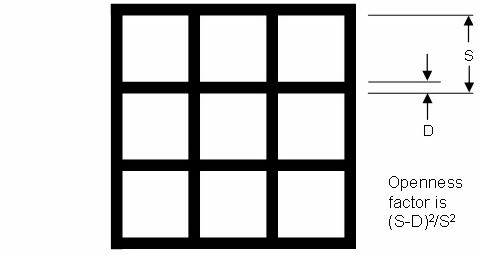
\includegraphics[width=0.9\textwidth, height=0.9\textheight, keepaspectratio=true]{media/image1153.png}
\caption{Physical screen material properties \protect \label{fig:physical-screen-material-properties}}
\end{figure}

\subsection{Screen Properties and Calculations}\label{screen-properties-and-calculations}

\subsubsection{Screen Beam Transmittance}\label{screen-beam-transmittance}

The first component of the window screen transmittance model is a geometric representation of the open area of the screen material and is dependent on the angle of incident beam radiation. Figure~\ref{fig:schematic-of-a-vertical-window-screen-facing} shows a schematic of a South-facing vertical window screen and the solar angles used in EnergyPlus. The window screen model is based on the relative angles of incidence of the sun's rays with respect the the window screen outward normal. In the figure, the relative solar azimuth and relative solar altitude are represented as φ' and α', respectively.

\begin{figure}[hbtp] % fig 87
\centering
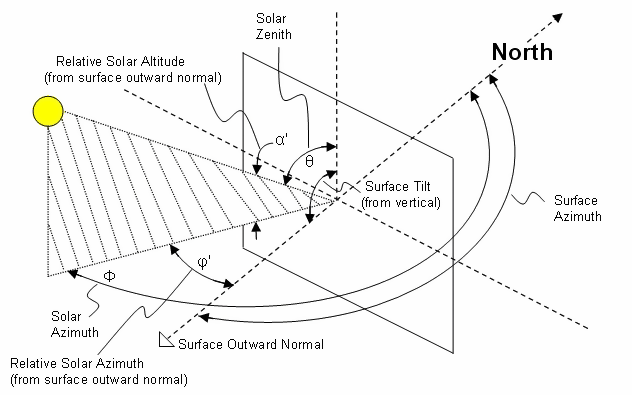
\includegraphics[width=0.9\textwidth, height=0.9\textheight, keepaspectratio=true]{media/image1154.png}
\caption{Schematic of a vertical window screen facing due South \protect \label{fig:schematic-of-a-vertical-window-screen-facing}}
\end{figure}

Given the diffuse reflectance ρ\(_{sc}\) and the screen aspect ratio γ, the model takes the direction of solar incidence, the relative solar altitude angle α' and the relative solar azimuth angle φ', illustrated in Figure~\ref{fig:schematic-of-a-vertical-window-screen-facing}, and calculates the direct beam transmittance \emph{T\(_{beam}\)} (α', φ') as follows. Since the direct beam transmittance is only a function of the incident angle and the screen material aspect ratio, the following applies to both solar and visible radiation.

\begin{equation}
\alpha '' = {\rm{arctan}}\left( {\tan \alpha '\sec \varphi '} \right)
\end{equation}

\begin{equation}
\beta  = \frac{\pi }{2} - \varphi '
\end{equation}

\begin{equation}
{T_y} = 1 - \gamma \left[ {\cos \alpha '' + \sin \alpha ''\tan \alpha '{{\left( {1 + {{\cot }^2}\beta } \right)}^{\frac{1}{2}}}} \right]
\end{equation}

\begin{equation}
\mu  = \arccos \left( {{{\left[ {{{\cos }^2}\alpha '{{\cos }^2}\varphi ' + {{\sin }^2}\alpha '} \right]}^{\frac{1}{2}}}} \right)
\end{equation}

\begin{equation}
  \varepsilon  = \arccos \PB{\frac{\cos \alpha '\cos \varphi '}{\cos \mu}}
\end{equation}

\begin{equation}
\eta  = \frac{\pi }{2} - \varepsilon
\end{equation}

\begin{equation}
\mu ' = \arctan \left( {\tan \mu \sec \varepsilon } \right)
\end{equation}

\begin{equation}
{T_x} = 1 - \gamma \left[ {\cos \mu ' + \sin \mu '\tan \mu {{\left( {1 + {{\cot }^2}\eta } \right)}^{\frac{1}{2}}}} \right]
\end{equation}

\begin{equation}
{T_{beam}}\left( {\alpha ',\varphi '} \right) = T_{beam}^{vis}\left( {\alpha ',\varphi '} \right) = {T_x}{T_y}
\end{equation}

where

\({T_y}\) ~ = vertical component of direct beam transmittance

\({T_x}\) ~ = horizontal component of direct beam transmittance

\({T_{beam}}\) ~ = direct screen transmittance that accounts for beam solar radiation passing through the screen openings without hitting the screen material

\(T_{beam}^{vis}\) ~ = direct visible screen transmittance that accounts for beam solar radiation passing through the screen openings without hitting the screen material

α'~~ = relative solar altitude angle {[}radians{]}

φ'~~ = relative solar azimuth angle {[}radians{]}

\(\gamma\) ~~ = Screen material aspect ratio, dimensionless

\(\alpha '',\beta ,\mu ,\varepsilon ,\eta ,\mu '\) ~ = intermediate variables

This first component of screen direct beam transmittance was developed using geometric principals and was verified using an optical ray tracing software program.

The second component of the window screen transmittance model is an empirical algorithm that accounts for the inward reflection of incident beam radiation off the screen material surface. The calculation procedure for the screen's transmittance via beam reflection, \emph{T\(_{scatt}\)} (α', φ') is as follows:

\begin{equation}
\begin{array}{l}{T_{scattmax}} = 0.0229\,\gamma  + 0.2971\,{\rho_{sc}} - 0.03624\,{\gamma ^2}\, + \\\,\,\,\,\,\,\,\,\,\,\,\,\,\,\,\,\,\,\,\,0.04763\,{\rho_{sc}}^2 - 0.44416\,\gamma \,{\rho_{sc}}\end{array}
\end{equation}

\begin{equation}
\begin{array}{l}T_{scattmax}^{vis} = 0.0229\,\gamma  + 0.2971\,\rho_{sc}^{vis} - 0.03624\,{\gamma ^2}\, + \\\,\,\,\,\,\,\,\,\,\,\,\,\,\,\,\,\,\,\,\,0.04763{\left( {\rho_{sc}^{vis}} \right)^2} - 0.44416\,\gamma \,\rho_{sc}^{vis}\end{array}
\end{equation}

\begin{equation}
{\delta_{max}} = 89.7 - {{10\gamma } \mathord{\left/ {\vphantom {{10\gamma } {0.16}}} \right. } {0.16}}
\end{equation}

\begin{equation}
\delta  = {\left( {\alpha_d^{'2} + \varphi_d^{'2}} \right)^{\frac{1}{2}}}
\end{equation}

\begin{equation}
  Peak_{ratio} = \frac{1}{0.2{\rho_{sc}}\left( {1 - \gamma } \right)}
\end{equation}

\begin{equation}
  Peak_{ratio}^{vis} = \frac{1}{0.2\rho_{sc}^{vis}\left( {1 - \gamma } \right)}
\end{equation}

\begin{equation}
{T_{scatt}}\left( {\alpha ',\varphi '} \right) = 0.2{\rho_{sc}}{T_{scattmax}}\left( {1 - \gamma } \right)\left( {1 + \left( {Pea{k_{ratio}} - 1} \right){e^{\frac{{ - {{\left| {\delta  - {\delta_{max}}} \right|}^{2.0}}}}{{600}}}}} \right)
\end{equation}

\begin{equation}
T_{scatt}^{vis}\left( {\alpha ',\varphi '} \right) = 0.2\rho_{sc}^{vis}T_{scattmax}^{vis}\left( {1 - \gamma } \right)\left( {1 + \left( {Peak_{ratio}^{vis} - 1} \right){e^{\frac{{ - {{\left| {\delta  - {\delta_{max}}} \right|}^{2.0}}}}{{600}}}}} \right)
\end{equation}

If $\delta > \delta_{max}$, then:

\begin{equation}
  \begin{array}{rl}
    T_{scatt} \left( \alpha ',\varphi ' \right) &= 0.2 \rho_{sc} T_{scattmax} \left( 1 - \gamma \right) \left( 1 + \left( Peak_{ratio} - 1 \right) e^{\frac{- \left| \delta - \delta_{max} \right|^{2.5}}{600}} \right) \\
                                                &- 0.2 \rho_{sc} T_{scattmax} \left( 1 - \gamma \right) \left( \max \left( 0.0, \frac{\delta  - \delta_{max}}{90. - {delta_{max}}} \right) \right) \\
    T_{scatt}^{vis} \left( \alpha ',\varphi ' \right) &= 0.2 \rho_{sc}^{vis} T_{scattmax}^{vis} \left( 1 - \gamma \right) \left( 1 + \left( Peak_{ratio}^{vis} - 1 \right) e^{\frac{- \left| \delta - \delta_{max} \right|^{2.5}}{600}} \right) \\
                                                      &- 0.2 \rho_{sc}^{vis} T_{scattmax}^{vis} \left( 1 - \gamma \right) \left( \max \left( 0.0, \frac{\delta  - \delta_{max}}{90. - {delta_{max}}} \right) \right)
  \end{array}
\end{equation}

where

\({T_{scattmax}}\) ~ = maximum reflected (scattered) beam transmittance

\(T_{scattmax}^{vis}\) ~ = maximum visible reflected (scattered) beam transmittance

\({\delta_{max}},\delta\) ~ = intermediate variables {[}degrees{]}

\(\alpha_d'\) ~ = relative solar altitude {[}degrees{]}

\(\varphi_d'\) ~ = relative solar azimuth {[}degrees{]}

\(Pea{k_{ratio}}\) = Ratio of peak scattered beam transmittance to scattered beam transmittance at direct normal incidence.

\(Peak_{ratio}^{vis}\) = Ratio of peak scattered visible transmittance to scattered visible transmittance at direct normal incidence.

\({\rho_{sc}}\) = diffuse solar reflectance of the screen material

\(\rho_{sc}^{vis}\) = diffuse visible reflectance of the screen material

\({T_{scatt}}\) ~ = beam solar transmittance due to reflectance (scattering)

\(T_{scatt}^{vis}\) ~ = beam visible transmittance due to reflectance (scattering)

The reflected (scattered) transmittance of incident beam radiation is an empirical model derived by curvefitting results from optical ray trace modeling. Ray traces were performed for a range of screen aspect ratios, diffuse screen reflectances, and relative solar azimuth and altitude angles. The surface of the screen cylinders was assumed to be diffusely reflecting, having the optical properties of a Lambertian surface. The transmitted flux due to reflection was determined by a hemispherical detector on the transmitted side of the screen.

These two components of beam solar transmittance are then used to specify the properties for beam-to-beam and beam-to-diffuse transmittance for the screen based on the user selection for Reflected Beam Transmittance Accounting Method in the WindowMaterial:Screen object. The calculations below apply to both the solar and visible beam solar transmittance.

If the user selects DoNotModel, the direct beam transmittance is set to \emph{T\(_{beam}\)} and the reflected (scattered) portion of the beam solar transmittance is ignored:

\begin{equation}
T_{sc}^{dir,dir} = {T_{beam}}\left( {\alpha ',\varphi '} \right)
\end{equation}

\begin{equation}
T_{sc}^{dir,dif} = 0.0
\end{equation}

\begin{equation}
T_{sc,\,vis}^{dir,dir} = {T_{beam}}\left( {\alpha ',\varphi '} \right)
\end{equation}

\begin{equation}
T_{sc,\,vis}^{dir,dif} = 0.0
\end{equation}

where

\(T_{sc}^{dir,dir}\) ~ = direct-to-direct beam transmittance of the screen (output report variable Surface Window Screen Beam to Beam Solar Transmittance)

\(T_{sc}^{dir,dif}\) = direct-to-diffuse beam transmittance of the screen (output report variable Surface Window Screen Beam to Diffuse Solar Transmittance)

\(T_{sc,\,vis}^{dir,dir}\) ~ = direct-to-direct visible transmittance of the screen

\(T_{sc,\,vis}^{dir,dif}\) = direct-to-diffuse visible transmittance of the screen

If the user selects Model as Direct Beam, the reflected (scattered) portion of the beam solar transmittance is added to the direct beam transmittance \emph{T\(_{beam}\)} in the same solid angle and direction of the unattenuated solar beam:

\begin{equation}
T_{sc}^{dir,dir} = {T_{beam}}\left( {\alpha ',\varphi '} \right) + {T_{scatt}}\left( {\alpha ',\varphi '} \right)
\end{equation}

\begin{equation}
T_{sc}^{dir,dif} = 0.0
\end{equation}

\begin{equation}
T_{sc,\,vis}^{dir,dir} = {T_{beam}}\left( {\alpha ',\varphi '} \right) + T_{scatt}^{vis}\left( {\alpha ',\varphi '} \right)
\end{equation}

\begin{equation}
T_{sc,\,vis}^{dir,dif} = 0.0
\end{equation}

If the user selects Model as Diffuse Beam, the direct beam transmittance is set to \emph{T\(_{beam}\)} and the reflected (scattered) portion of the beam solar transmittance is modeled as diffuse hemispherical radiation:

\begin{equation}
T_{sc}^{dir,dir} = {T_{beam}}\left( {\alpha ',\varphi '} \right)
\end{equation}

\begin{equation}
T_{sc}^{dir,dif} = {T_{scatt}}\left( {\alpha ',\varphi '} \right)
\end{equation}

\begin{equation}
T_{sc,\,vis}^{dir,dir} = {T_{beam}}\left( {\alpha ',\varphi '} \right)
\end{equation}

\begin{equation}
T_{sc,\,vis}^{dir,dif} = T_{scatt}^{vis}\left( {\alpha ',\varphi '} \right)
\end{equation}

\subsubsection{Screen Beam Reflectance}\label{screen-beam-reflectance}

The screen reflectance (overall value for the screen assembly, accounting for the screen material itself and the open spaces between the screen material) is calculated by first subtracting the direct-to-direct screen transmittance from the unit incident beam. This approximates the fraction of incident beam solar radiation striking the screen that is not inwardly transmitted. The result is then multiplied by the screen material diffuse reflectance ρ\(_{sc}\). The inwardly scattered transmittance is then subtracted from this quantity to obtain an approximate value for the screen's reflectance R\(_{sc}\) to beam radiation incident as a function of the relative angles of incident radiation. This equation is used for both beam and visible reflectance:

\begin{equation}
R_{SC}^{dir,dif}\left( {\alpha ',\varphi '} \right) = {\rho_{SC}}\left( {1 - T_{SC}^{dir,dir}} \right) - T_{SC}^{dir,dif}
\end{equation}

\begin{equation}
R_{SC,vis}^{dir,dif}\left( {\alpha ',\varphi '} \right) = \rho_{SC}^{vis}\left( {1 - T_{SC,vis}^{dir,dir}} \right) - T_{SC,vis}^{dir,dif}
\end{equation}

\subsubsection{Screen Beam Absorptance}\label{screen-beam-absorptance}

The screen absorptance(overall value for the screen assembly, accounting for the screen material itself and the open spaces between the screen material) is calculated as the quantity of the unit incident flux (1) less the directly-transmitted component \emph{T\(_{dir,dir}\)} multiplied by the quantity 1 minus the screen material diffuse reflectance.

\begin{equation}
A_{SC}^{dir}\left( {\alpha ',\varphi '} \right) = \left( {1 - T_{SC}^{dir,dir}} \right)\left( {1 - {\rho_{SC}}} \right)
\end{equation}

\subsubsection{Screen Diffuse Properties}\label{screen-diffuse-properties}

The transmittance of the screen to half-hemispherical diffuse (sky) radiation is calculated by performing a finite-element-summation, approximately equivalent to an integration over the solid angle of the beam transmittance, assuming uniform radiance. This single-number screen diffuse transmittance is then multiplied by the irradiance incident on the screen from a uniform half-hemisphere of sky- or ground-reflected radiation to determine the level of additional flux transmitted by the screen to the window from the diffuse sky or ground. The sun angles shown in the figure below represent the solar altitude angle (θ) and solar azimuth angle (Ф) in polar coordinates. These angles are used to calculate the average diffuse-to-diffuse properties for screens in the following derivations.

\begin{figure}[hbtp] % fig 88
\centering
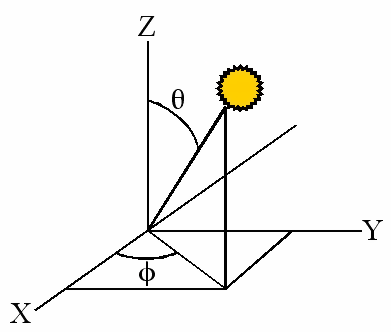
\includegraphics[width=0.9\textwidth, height=0.9\textheight, keepaspectratio=true]{media/image1210.png}
\caption{Sun Angles in Screen Calculations. \protect \label{fig:sun-angles-in-screen-calculations.}}
\end{figure}

The screen transmittance to diffuse radiation \emph{T\(_{dif,dif}\)} (γ, ρ\(_{sc}\))~ is computed as the integrated average of the combined beam transmittance \emph{T\(_{tot}\)} (γ, ρ, θ, Ф) over the directions of incidence using spherical coordinates (θ, Ф) in which the z-axis is perpendicular to the plane of the screen. Using a finite element computation, this is:

\begin{equation}
{T_{tot}}(\gamma ,{\rho_{sc}},{\theta_j},{\phi_i}) = {T_{beam}}\left( {\alpha ',\varphi '} \right) + {T_{scatt}}\left( {\alpha ',\varphi '} \right)
\end{equation}

\begin{equation}
T_{sc}^{dif,dif}(\gamma ,{\rho_{sc}}) = \frac{{\sum\limits_{j = 1}^N {\sum\limits_{i = 1}^M {{T_{tot}}(\gamma ,{\rho_{sc}},{\theta_j},{\phi_i})\sin ({\theta_j})\cos ({\theta_j})} } }}{{\sum\limits_{j = 1}^N {\sum\limits_{i = 1}^M {\sin ({\theta_j})\cos ({\theta_j})} } }}
\end{equation}

where

\(\theta\) ~ = solar altitude angle in polar coordinates {[}radians{]}

\(\phi\) ~ = solar azimuth angle in polar coordinates {[}radians{]}

\(T_{sc}^{dif,dif}(\gamma ,{\rho_{sc}})\) = diffuse-diffuse transmittance (output report variable Surface Window Screen Diffuse to Diffuse Solar Transmittance)

Similarly, the reflectance of the screen to diffuse radiation is given by

\begin{equation}
R_{sc}^{dif,dif}(\gamma ,{\rho_{sc}}) = \frac{{\sum\limits_{j = 1}^N {\sum\limits_{i = 1}^M {R_{sc}^{dir,dif}(\gamma ,{\rho_{sc}},{\theta_j},{\phi_i})\sin ({\theta_j})\cos ({\theta_j})} } }}{{\sum\limits_{j = 1}^N {\sum\limits_{i = 1}^M {\sin ({\theta_j})\cos ({\theta_j})} } }}
\end{equation}

There is an assumption in both of these formulas that the brightness of the sky (or ground) diffuse radiation is the same for all directions. For this reason, the solar azimuth angle Ф and solar altitude angle θ have a range of 0 to \({\pi \mathord{\left/ {\vphantom {\pi 2}} \right. } 2}\) ~(instead of \({{ - \pi } \mathord{\left/ {\vphantom {{ - \pi } 2}} \right. } 2}\) ~to \({{ + \pi } \mathord{\left/ {\vphantom {{ + \pi } 2}} \right. } 2}\) ) because the screen is assumed to have identical optical properties for radiation incident at the same angles on either side of a vertical or horizontal plane perpendicular to the screen.

Since the screen direct transmittance model is derived with respect to a different coordinate axis labeling, a coordinate transform is needed in order to calculate the diffuse optical properties. In these calculations, for each spherical solar coordinates (θ, Ф) we need the corresponding screen relative solar coordinates (α', φ') to evaluate the screen transmittance model for that direction.

For each θ and Ф in the summation, the corresponding values for the relative solar altitude α' and relative solar azimuth φ' needed to calculate screen transmittance are determined with the following coordinate transform equations:

\begin{equation}
\sin \alpha ' = \sin \theta \cos \phi
\end{equation}

\begin{equation}
\tan \varphi ' = \tan \theta \sin \phi
\end{equation}

The absorptance of the screen to diffuse incident radiation is calculated by subtracting the diffuse transmittance and diffuse reflectance from unity as follows:

\begin{equation}
A_{sc}^{dif}(\gamma ,{\rho_{sc}}) = 1 - T_{sc}^{dif,dif}(\gamma ,{\rho_{sc}}) - R_{sc}^{dif,dif}(\gamma ,{\rho_{sc}})
\end{equation}

\subsubsection{Screen/Glass System Properties for Short-Wave Radiation}\label{screenglass-system-properties-for-short-wave-radiation}

The combined system properties of the screen/glass combination are calculated using the properties of the screen in combination with the bare glass material properties. Interreflections of radiation between the screen and glass surfaces are included. The following infinite series serves as an example for calculating the combined screen/glass system properties. The terms of the series are built up as illustrated in the following figure. The terms shown at the right of the figure represent each term in the infinite series for the combined screen/glass property (beam transmittance in this example).

For the example of beam transmittance, the incident solar beam strikes the screen at the incident angle associated with the current relative azimuth and altitude angle. The incident beam splits into reflected and transmitted components at the screen. The transmitted component is attenuated as it passes through the screen material by the screen's beam transmittance (\(T_{sc}^{dir,dir}\) , shown as\(T_{sc}^{dir}\) ~in the figure and equations below) at this incident angle. The reflected (scattered) transmittance of incident solar beam is also shown at this point and will be discussed later in this section. As the attenuated solar beam continues on towards the front glass surface, a portion of the screen-transmitted beam splits at the window surface into transmitted and reflected components. The reflected component reflects off the front surface of the glass material (\(T_{sc}^{dir,dir}R_{gl,f}^{dir}\) ) and the transmitted component continues to travel through the glass material and is further attenuated by the glass beam transmittance. Thus the first term of the combined screen/glass solar beam transmittance is shown as \(T_{sc}^{dir,dir}T_{gl}^{dir}\) . Interreflections are accounted for by following the beam as it continues to reflect off the front surface of the glass material and the back surface of the screen material. Continuing on with the glass-reflected beam (\(T_{sc}^{dir,dir}R_{gl,f}^{dir}\) ) described above, this beam strikes the back surface of the screen material at the same incident angle as the incident solar beam. This reflected beam is also assumed to be a collimated beam (solid lines) which strikes the back surface of the screen material and reflects as hemispherically-diffuse radiation (dotted lines). The reflective property of the screen material used here is the beam reflectance calculated at the incident solar angle (\(R_{sc}^{dir,dif}\) ). A single ray of this diffuse light will be followed through the remaining steps and represents the energy associated with \textbf{all} diffuse rays interreflecting between the screen and glass layers. To determine the second term of the combined screen/glass beam transmittance, the diffusely-reflected ray (\(T_{sc}^{dir,dir}R_{gl,f}^{dir}R_{sc}^{dir,dif}\) ) passes through and is attenuated by the glass layer. Since this ray originates from diffuse reflection, the attenuation of this ray is accounted for using the diffuse transmittance property of the glass. Thus, the second term is shown as \(T_{sc}^{dir,dir}R_{gl,f}^{dir}R_{sc}^{dir,dif}T_{gl}^{dif}\) . Defining the remaining terms continues in a similar fashion using diffuse properties of both the screen and glass material. Notice that the 3\(^{rd}\) and 4\(^{th}\) terms shown below are similar to the 2\(^{nd}\) term, but additional terms are raised to increasing powers.

\begin{figure}[hbtp] % fig 89
\centering
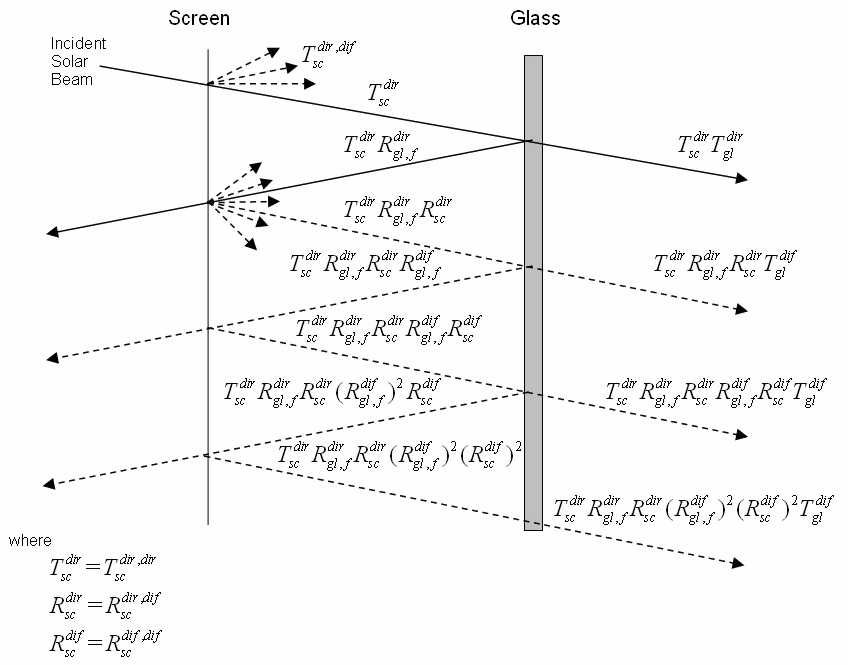
\includegraphics[width=0.9\textwidth, height=0.9\textheight, keepaspectratio=true]{media/image1231.png}
\caption{Screen/Glass System Transmittance Equation Schematic. \protect \label{fig:screenglass-system-transmittance-equation}}
\end{figure}

The screen/glass system transmittance equation shown in the figure above is repeated here in an alternate format to emphasize the recurring nature of the infinite series. This equation represents the final solar beam transmittance equation for the screen/glass combination. The recurring terms are shown as a summation of a quantity raised to the n power, with n ranging from 0 to infinity. Since the quantity \(R_{gl}^{dif}R_{sc}^{dif,dif}\) ~is less than 1, the summation \(\sum\limits_{n = 0}^\infty {{{(R_{gl,f}^{dif}R_{sc}^{dif,dif})}^n}}\) converges and can be expressed as $\PB{1-R_{gl,f}^{dif}R_{sc}^{dif,dif}}^{-1}$.  Since the reflected (scattered) transmittance of incident solar beam (\(T_{sc}^{dir,dif}\)) and the diffusely reflecting beam \(T_{sc}^{dir,dir}R_{gl,f}^{dir}R_{sc}^{dir,dif}\) ~are both assumed to be hemispherically diffuse radiation, the reflected (scattered) transmittance of incident solar beam is added to the infinite series as shown below.

\begin{equation}
\begin{array}{rl}
  T_{sys}^{dir,all}(\alpha ',\varphi ',\phi ) &= T_{sc}^{dir,dir}(\alpha ',\varphi ')T_{gl}^{dir}\left( \phi  \right) \\
                                              &+ (T_{sc}^{dir,dir}(\alpha ',\varphi ')R_{gl,f}^{dir}R_{sc}^{dir,dif}(\alpha ',\varphi ') \\
                                              &+ T_{sc}^{dir,dif}(\alpha ',\varphi '))T_{gl}^{dif}\sum\limits_{n = 0}^\infty  {{{(R_{gl,f}^{dif}R_{sc}^{dif,dif})}^n}} 
\end{array}
\end{equation}

or:

\begin{equation}
T_{sys}^{dir,all}(\alpha ',\varphi ',\phi ) = T_{sc}^{dir,dir}(\alpha ',\varphi ')T_{gl}^{dir}\left( \phi  \right) + \frac{{(T_{sc}^{dir,dir}(\alpha ',\varphi ')R_{gl,f}^{dir}R_{sc}^{dir,dif}(\alpha ',\varphi ') + T_{sc}^{dir,dif}(\alpha ',\varphi '))T_{gl}^{dif}}}{{1 - R_{gl,f}^{dif}R_{sc}^{dif,dif}}}
\end{equation}

where

\(T_{sys}^{dir,all}(\alpha ',\varphi ',\phi )\) ~ = screen/glass system beam transmittance (output report variable Surface Window Screen and Glazing System Beam Solar Transmittance)

Properties for beam absorptance of the individual glass layers and screen/glass combination are derived in a similar fashion to the transmittance calculation described above. Diffuse transmittance and absorptance of individual glass layers and the screen/glass combination are also shown here.

\begin{equation}
\begin{array}{l}A_{gl,j,f}^{dir,sys}\left( {\alpha ',\varphi ',\phi } \right) = T_{sc}^{dir,dir}\left( {\alpha ',\varphi '} \right)A_{gl,j,f}^{dir}\left( \phi \right) + \\\;\;\;\;\;\;\;\;\;\;\;\;\;\;\,\,\,\,\,\,\,\,\,\,\,\,\,\,\,\,\,\,\,\,\;\;\;\;\;\;\frac{{\left( {T_{sc}^{dir,dir}\left( {\alpha ',\varphi '} \right)R_{gl}^{dir}\left( \phi \right)R_{sc}^{dir,dif}\left( {\alpha ',\varphi '} \right) + T_{sc}^{dir,dif}\left( {\alpha ',\varphi '} \right)} \right)A_{gl,j,f}^{dif}}}{{1 - R_{gl,f}^{dif}R_{sc}^{dif,dif}}},\;j = 1,N\end{array}
\end{equation}

\begin{equation}
\begin{array}{l}\alpha_{sc}^{dir,sys}\left( {\alpha ',\varphi ',\phi } \right) = A_{sc}^{dir}\left( {\alpha ',\varphi '} \right)\left( {1 + R_{gl,f}^{dir}\left( \phi \right)T_{sc}^{dir,dir}\left( {\alpha ',\varphi '} \right)} \right) + \\\;\;\;\;\;\;\;\;\;\;\;\;\;\;\;\;\;\;\;\;\;\;\;\;\;\;\;\;\;\;\;\frac{{A_{sc}^{dif}R_{gl,f}^{dif}}}{{1 - R_{sc}^{dif,dif}R_{gl,f}^{dif}}}\left( {R_{gl,f}^{dir}\left( \phi \right)T_{sc}^{dir,dir}\left( {\alpha ',\varphi '} \right)R_{sc}^{dir,dif}\left( {\alpha ',\varphi '} \right)} \right)\end{array}
\end{equation}

\begin{equation}
T_{sys}^{dif,dif} = \frac{{T_{sc}^{dif,dif}T_{gl}^{dif}}}{{1 - R_{gl,f}^{dif}R_{sc}^{dif,dif}}}
\end{equation}

\begin{equation}
A_{gl,j,f}^{dif,sys} = \frac{{T_{sc}^{dif,dif}A_{gl,j,f}^{dif}}}{{1 - R_{gl,f}^{dif}R_{sc}^{dif,dif}}},\;j = 1,N
\end{equation}

\begin{equation}
\alpha_{sc}^{dif,\,sys} = A_{sc}^{dif}\left( {1 + \frac{{T_{sc}^{dif,dif}R_{gl,f}^{dif}}}{{1 - R_{gl,f}^{dif}R_{sc}^{dif,dif}}}} \right)
\end{equation}

where

\(A_{gl,j,f}^{dir,sys}\left( {\alpha ',\varphi ',\phi } \right)\) ~ = glass layer beam absorptance including interreflections with screen material

\(\alpha_{sc}^{dir,sys}\left( {\alpha ',\varphi ',\phi } \right)\) ~ = beam absorptance of screen material including interreflections with glass

\(T_{sys}^{dif,dif}\) ~ = screen/glass system diffuse transmittance (output report variable Surface Window Screen and Glazing System Diffuse Solar Transmittance)

\(A_{gl,j,f}^{dif,sys}\) ~ = glass layer diffuse absorptance including interreflections with screen material

\(\alpha_{sc}^{dif,sys}\) ~ = diffuse absorptance of screen material including interreflections with glass

\subsubsection{Screen/Glazing System Properties for Long-Wave Radiation}\label{screenglazing-system-properties-for-long-wave-radiation}

The program calculates how much long-wave radiation is absorbed by the screen and by the adjacent glass surface. The effective long-wave emissivity (equal to the long-wave absorptance on a wavelength-by-wavelength basis or over the same spectral range) of an exterior screen, taking into account reflection of long-wave radiation between the glass and screen, is given by

\begin{equation}
\varepsilon_{sc}^{lw,eff} = \varepsilon_{sc}^{lw}\left( {1 + \frac{{T_{sc}^{dif,dif}\rho_{gl}^{lw}}}{{1 - R_{sc}^{dif,dif}\rho_{gl}^{lw}}}} \right)
\end{equation}

where \(\rho_{gl}^{lw}\) is the long-wave reflectance of the outermost glass surface facing an exterior screen, and it is assumed that the long-wave transmittance of the glass is zero.

The effective outermost (for exterior screen) glass surface emissivity when the screen is present is

\begin{equation}
\varepsilon_{gl}^{lw,eff} = \varepsilon_{gl}^{lw}\frac{{T_{sc}^{dif,dif}}}{{1 - R_{sc}^{dif,dif}\rho_{gl}^{lw}}}
\end{equation}

The effective inside surface emissivity is the sum of the effective screen and effective glass emissivities:

\begin{equation}
\varepsilon_{ins}^{lw,eff} = \varepsilon_{sc}^{lw,eff} + \varepsilon_{gl}^{lw,eff}
\end{equation}

The effective temperature of the screen/glazing combination that is used to calculate the window's contribution to the zone's mean radiant temperature (MRT) is given by

\begin{equation}
{T^{eff}} = \frac{{\varepsilon_{sc}^{lw,eff}{T_{sc}} + \varepsilon_{gl}^{lw,eff}{T_{gl}}}}{{\varepsilon_{sc}^{lw,eff} + \varepsilon_{gl}^{lw,eff}}}
\end{equation}

\subsubsection{Solar Radiation Transmitted and Absorbed by a Window/Screen System}\label{solar-radiation-transmitted-and-absorbed-by-a-windowscreen-system}

Let the direct solar incident on the window be

\begin{equation}
{I_{dir,inc}} = {f_{sunlit}}{I_{dir,norm}}\cos \phi {\rm{    }}(W/{m^2})
\end{equation}

where \({f_{sunlit}}\) is the fraction of the window that is sunlit (determined by the shadowing calculations), \({I_{dir,norm}}\) is the direct normal solar irradiance, and \(\phi\) ~is the angle of incidence.

Let \({I_{sky,inc}}\) be the irradiance on the window due to diffuse solar radiation from the sky (W/m\(^{2}\)) and let \({I_{gnd,inc}}\) be the irradiance on the window due to diffuse solar radiation from the ground (W/m\(^{2}\)).

Then we have the following expressions for different classes of transmitted and absorbed solar radiation for the window/screen system, all in W/m\(^{2}\):

\emph{Direct and diffuse solar entering zone from incident direct solar:}

\begin{equation}
{I_{dir,inc}}T_{sys}^{dir,all}\left( {\alpha ',\varphi '} \right)
\end{equation}

\emph{Direct solar absorbed by screen:}

\begin{equation}
{I_{dir,inc}}\alpha_{sc}^{dir,sys}\left( {\alpha ',\varphi '} \right)
\end{equation}

\emph{Direct solar absorbed by glass layers:}

\begin{equation}
{I_{dir,inc}}A_{gl,j,f}^{dir,sys}(\phi ,{\phi_s}),{\rm{    }}j = 1,N
\end{equation}

\emph{Diffuse solar entering zone from incident diffuse solar:}

\begin{equation}
\left( {{I_{sky,inc}} + {I_{gnd,inc}}} \right)T_{sys}^{dif,dif}
\end{equation}

\emph{Diffuse solar absorbed by screen:}

\begin{equation}
\left( {Isky,inc + Ignd,inc} \right)\alpha_{sc}^{dif,sys}
\end{equation}

\emph{Diffuse solar absorbed by glass layers:}

\begin{equation}
({I_{sky,inc}} + {I_{gnd,inc}})A_{gl,j,f}^{dif,sys},{\rm{   }}j = 1,N{\rm{ }}
\end{equation}

\subsection{Complex Fenestration Calculation Module}\label{complex-fenestration-calculation-module}

This section describes detailed method for modeling complex fenestration systems, including shading devices and general fenestration attachments. This detailed method primarily refers to the optical side of modeling complex fenestration systems. Thermal modeling is done according to ISO 15099 standard, which is described in the Window Heat Balance Calculation section with the addition of deflection and vacuum glazing systems modeling and some modifications to shading layer algorithms, which is described in Shading Device Thermal Model section. Optical caclulations in this method are done using Bidirectional Scattering Distribution Function (BSDF) approach.~ The concept behind BSDF is based on the definition of descrete set of incident and outgoing angles, which fully describes optical performance of any system, simple or complex, limited only by the resolution of angular discretization.~ In this method each layer, as well as the whole system is described by a matrix of incident and outgoing angles.

\subsubsection{Complex Fenestration Solar-Optical Calculations}\label{complex-fenestration-solar-optical-calculations}

\paragraph{\texorpdfstring{\textbf{Solar radiation calculation outline}}{Solar radiation calculation outline}}\label{solar-radiation-calculation-outline}

For solar radiation calculations, each of the layers as well as entire glazing system can be represented with the set of Bi-directional Scattering Distribution Functions or BSDF, consisting of Bi-directional Reflectance Distribution Function or BRDF and Bi-directional Transmittance Distribution Function or BTDF.~ Each function is a matrix 145 x 145 that describes reflectance or transmittance distribution in the outgoing hemisphere for each incident angle in the incidence hemisphere.~ For each function there is forward and back matrix, for a total of 4 145 x 145 matrices.~ Depending on the purpose of calculations, description of entire glazing system is divided into solar and visible spectrum, which means that there can be 8 matrices describing visible and complete solar spectrums.~ Reflectance and transmittance being non-dimnsional ratios of reflected or transmitted energy over incident energy, in order to get total reflected and transmitted energy it is necessary to supply vector of incident solar energy, which usually consists of direct and diffuse radition.Specifics of calculations of direct and diffuse solar radiationis be described in some detail in oncoming chapters.

\subparagraph{\texorpdfstring{\textbf{Scattering (Non-Specular) Glazing and Shading Devices}}{Scattering (Non-Specular) Glazing and Shading Devices}}\label{scattering-non-specular-glazing-and-shading-devices}

A general scattering fenestration system is characterized by BTDFs and BRDFs, which were described above.~ Given an incident direction \textbf{\emph{p}}\(^{(I)}\), and an incident irradiance \emph{E}( \textbf{\emph{p}}\(^{(I)}\)), the transmitted radiance in the outgoing direction \textbf{\emph{p}}\(^{(T)}\) is

\begin{equation}
S({{\bf{p}}^{{\rm{(T)}}}}) = {\mathop{\rm T}\nolimits} ({{\bf{p}}^{{\rm{(T)}}}},{{\bf{p}}^{{\rm{(I)}}}})dE({{\bf{p}}^{{\rm{(I)}}}})
\end{equation}

where the function T is the BTDF.~ In the absence of a source of effectively plane-parallel incident radiation (such as direct sunlight) d\emph{E(\textbf{p}}\(^{(I)}\)\emph{)} is an infinitesimal quantity, and the right side of the equation must be summed over the irradiance from all incident directions to produce the outgoing radiance:

\begin{equation}
S({{\bf{p}}^{{\rm{(T)}}}}) = \int {{\mathop{\rm T}\nolimits} ({{\bf{p}}^{{\rm{(T)}}}},{{\bf{p}}^{{\rm{(I)}}}})\frac{{dE({{\bf{p}}^{{\rm{(I)}}}})}}{{d\Omega }}d\Omega }
\end{equation}

A similar equation gives the reflected radiance in the direction \textbf{\emph{p}}\(^{(R)}\):

\begin{equation}
S({{\bf{p}}^{{\rm{(R)}}}}) = \int {{\mathop{\rm R}\nolimits} ({{\bf{p}}^{{\rm{(R)}}}},{{\bf{p}}^{{\rm{(I)}}}})\frac{{dE({{\bf{p}}^{{\rm{(I)}}}})}}{{d\Omega }}d\Omega }
\end{equation}

We can express the irradiance in terms of the exterior luminance, S, in that direction,

\begin{equation}
dE({{\bf{p}}^{{\rm{(I)}}}})dA = {S^{{\rm{(I)}}}}({{\bf{p}}^{{\rm{(I)}}}})\left( { - {{\bf{p}}^{{\rm{(I)}}}}\cdot {\bf{n}}} \right)d{\Omega ^{{\rm{(I)}}}}dA
\end{equation}

\begin{figure}[hbtp] % fig 90
\centering
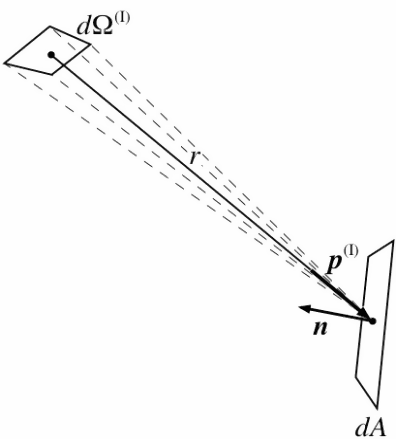
\includegraphics[width=0.9\textwidth, height=0.9\textheight, keepaspectratio=true]{media/image1271.png}
\caption{Irradiance geometry \protect \label{fig:irradiance-geometry}}
\end{figure}

which allows one to express the transmittance of exterior radiation to produce the total outgoing radiance from the fenestration into the room in a particular direction:

\begin{equation}
S({{\bf{p}}^{{\rm{(T)}}}}) = \int\limits_{{\Omega ^{{\rm{(I)}}}}} {{\mathop{\rm T}\nolimits} ({{\bf{p}}^{{\rm{(T)}}}},{{\bf{p}}^{{\rm{(I)}}}}){S^{{\rm{(I)}}}}({{\bf{p}}^{{\rm{(I)}}}})\left( { - {{\bf{p}}^{{\rm{(I)}}}}\cdot {\bf{n}}} \right)d{\Omega ^{{\rm{(I)}}}}}
\end{equation}

The negative sign is added to account for the fact that \textbf{\emph{p}}\(^{(I)}\) and \textbf{\emph{n}} have opposite sign for incoming radiation.

The radiance in equation is emitted from the back side of the element of area shown in Figure~\ref{fig:irradiance-geometry}.~ Considering a second surface, viewing the back side of the fenestration system, we can use equation to calculate the irradiance on surface 2,

\begin{equation}
{E^{{\rm{(2)}}}}({{\bf{p}}^{{\rm{(T)}}}})d{A^{{\rm{(2)}}}} = {S^{{\rm{(T)}}}}({{\bf{p}}^{{\rm{(T)}}}})\left( { - {{\bf{p}}^{{\rm{(T)}}}}\cdot {{\bf{n}}^{{\rm{(2)}}}}} \right)d{\Omega ^{{\rm{(I,2)}}}}d{A^{{\rm{(2)}}}}
\end{equation}

This expression, however, contains a number of new quantities, such as \(d{\Omega ^{{\rm{(I,2)}}}}\) , the element of solid angle for incoming radiation as seen from surface 2.~ We can sort this out by referring to Figure~\ref{fig:radiation-exchange-between-two-surface} and making some changes and clarifications in notation.

\begin{figure}[hbtp] % fig 91
\centering
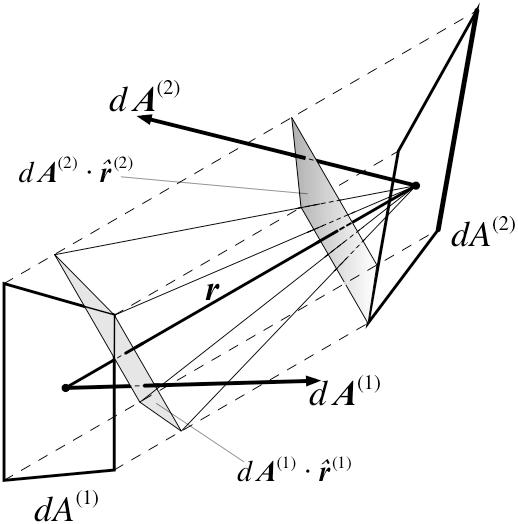
\includegraphics[width=0.9\textwidth, height=0.9\textheight, keepaspectratio=true]{media/image1275.png}
\caption{Radiation exchange between two surface elements \protect \label{fig:radiation-exchange-between-two-surface}}
\end{figure}

In this figure we consider that surface 1 is the back side of the fenestration system, and surface 2 is some other surface in the room that receives the transmitted solar radiation through the fenestration system.~ We consider infinitesimal elements \emph{dA}\(^{(1)}\) and \emph{dA}\(^{(2)}\) of the two surfaces, and define vector surface elements by \emph{d\textbf{A}}\textbf{\(^{(}\)}\(^{1)}\) = \emph{dA}\(^{(1)}\)\textbf{\emph{n}}\(^{(1)}\) and \emph{d\textbf{A}}\textbf{\(^{(}\)}\(^{1)}\) = \emph{dA}\(^{(1)}\)\textbf{\emph{n}}\(^{(1)}\).~ The quantity \textbf{\emph{r}} in the figure denotes a vector pointing from surface 1 to surface 2, the magnitude of which is the distance \emph{r} between the two surface elements.~ This is used to define two unit vectors: \({{\bf{\hat r}}^{{\rm{(1)}}}} = {{\bf{r}} \mathord{\left/ {\vphantom {{\bf{r}} r}} \right. } r}\) ~is a unit vector pointing from surface element 1 to surface element 2, and \({{\bf{\hat r}}^{{\rm{(2)}}}} = - {{\bf{r}} \mathord{\left/ {\vphantom {{\bf{r}} r}} \right. } r}\) ~is a unit vector pointing from surface element 2 back to surface element 1.~ The unit vector \textbf{\emph{p}}\(^{(T)}\) in equation is in fact \({{\bf{\hat r}}^{{\rm{(1)}}}}\) .~ The shaded quadrilaterals in the figure are the projected area elements normal to \textbf{\emph{r}}.~ Since the areas are infinitesimal, all the radiation leaving one surface element and arriving at the other will be in the direction \textbf{\emph{r}}, so that all radiation will be contained within the parallelepiped defined by the dashed lines (parallel to \textbf{\emph{r}}) joining the corners of the two surface elements.~ It follows that the area \emph{dA}\(^{(2)}\)~ is not independent of \emph{dA}\(^{(1)}\).~ The figure also shows the solid angle that has been denoted \emph{d}W\(^{(I,2)}\) above, which is the solid angle subtended by \emph{dA}\(^{(1)}\) as seen from \emph{dA}\(^{(2)}\) and is given by

\begin{equation}
d{\Omega ^{{\rm{(I,2)}}}} = \frac{{d{{\bf{A}}^{{\rm{(1)}}}} \cdot {{\bf{r}}^{{\rm{(1)}}}}}}{{{r^2}}}
\end{equation}

The net power from surface element 1 to surface element 2 is

\begin{equation}
{W^{(1 \to 2)}} = \left( {{S^{{\rm{(1)}}}}({{{\bf{\hat r}}}^{{\rm{(1)}}}}) - {S^{{\rm{(2)}}}}({{{\bf{\hat r}}}^{{\rm{(2)}}}})} \right)\frac{{\left( {d{{\bf{A}}^{{\rm{(1)}}}} \cdot {{{\bf{\hat r}}}^{{\rm{(1)}}}}} \right)\left( {d{{\bf{A}}^{{\rm{(2)}}}} \cdot {{{\bf{\hat r}}}^{{\rm{(2)}}}}} \right)}}{{{r^2}}}
\end{equation}

where \({S^{{\rm{(1)}}}}({{\bf{\hat r}}^{{\rm{(1)}}}})\) ~is the radiance leaving surface element 1 in the direction of surface element 2, and vice-versa for \({S^{{\rm{(2)}}}}({{\bf{\hat r}}^{{\rm{(2)}}}})\) .~ In this case, the latter is zero and the former is the quantity called \emph{S}\(^{(T)}\)(\textbf{\emph{p}}\(^{(T)}\)) above.~ Given equation , we can recognize the quantity multiplying the radiance as the solid angle \emph{d}W\(^{(I,2)}\) times the projected area of surface element 2 perpendicular to \textbf{\emph{r}}.~ But the expression is symmetrical in the two surface elements, so we could also express it as

\begin{equation}
{W^{(1 \to 2)}} = {S^{{\rm{(T)}}}}({{\bf{p}}^{{\rm{(T)}}}})\left( {d{{\bf{A}}^{{\rm{(1)}}}} \cdot {{{\bf{\hat r}}}^{{\rm{(1)}}}}} \right)d{\Omega ^{{\rm{(T)}}}}
\end{equation}

where

\begin{equation}
d{\Omega ^{{\rm{(T)}}}} = \frac{{\left( {d{{\bf{A}}^{{\rm{(2)}}}} \cdot {{{\bf{\hat r}}}^{{\rm{(2)}}}}} \right)}}{{{r^2}}}
\end{equation}

The superscript (T) is used here because the solid angle element pertains to the direction \textbf{\emph{p}}\(^{(T)}\).~ In the particular case under discussion that restricts attention to those directions for which the outgoing radiation strikes surface element 2.~ We can now rewrite equation as

\begin{equation}
{E^{{\rm{(2)}}}}({{\bf{p}}^{{\rm{(T)}}}})d{A^{{\rm{(2)}}}} = {S^{{\rm{(T)}}}}({{\bf{p}}^{{\rm{(T)}}}})\left( {{{\bf{n}}^{{\rm{(1)}}}} \cdot {{{\bf{\hat r}}}^{{\rm{(1)}}}}} \right)d{\Omega ^{{\rm{(T)}}}}d{A^{{\rm{(1)}}}}
\end{equation}

and since, as can readily be seen from Figure~\ref{fig:radiation-exchange-between-two-surface}, \(\left( {d{{\bf{A}}^{{\rm{(1)}}}} \cdot {{{\bf{\hat r}}}^{{\rm{(1)}}}}} \right) = \left( {d{{\bf{A}}^{{\rm{(2)}}}} \cdot {{{\bf{\hat r}}}^{{\rm{(2)}}}}} \right)\) , this becomes

\begin{equation}
{E^{{\rm{(2)}}}}({{\bf{p}}^{{\rm{(T)}}}}) = {S^{{\rm{(T)}}}}({{\bf{p}}^{{\rm{(T)}}}})\left( { - {{\bf{p}}^{{\rm{(T)}}}} \cdot {{\bf{n}}^{{\rm{(2)}}}}} \right)d{\Omega ^{{\rm{(T)}}}}
\end{equation}

Substituting equation for \emph{S}\(^{(T)}\)(\textbf{\emph{p}}\(^{(T)}\), we obtain a propagation equation for outside radiation passing through the window and arriving at surface element 2:

\begin{equation}
E^{(2)}(\bf{p}^{(T)}) = \int_{\Omega^{(I)}} 
      \rm T (\bf{p}^{(T)},\bf{p}^{(I)}) 
      S^{(I)}(\bf{p}^{(I)})(-\bf{p}^{(I)}\cdot\bf{n}^{(I)})
      d\Omega^{(I)}(-\bf{p}^{(T)}\cdot\bf{n}^{(2)})d\Omega^{(T)}
\end{equation}

or, in terms involving only irradiance,

\begin{equation}
{E^{{\rm{(2)}}}}({{\bf{p}}^{{\rm{(T)}}}}) = \int\limits_{{\Omega ^{{\rm{(I)}}}}} {{\mathop{\rm T}\nolimits} ({{\bf{p}}^{{\rm{(T)}}}},{{\bf{p}}^{{\rm{(I)}}}})E({{\bf{p}}^{{\rm{(I)}}}})d{\Omega ^{{\rm{(I)}}}}} \left( { - {{\bf{p}}^{{\rm{(T)}}}} \cdot {{\bf{n}}^{{\rm{(2)}}}}} \right)d{\Omega ^{{\rm{(T)}}}}
\end{equation}

Comparing these two equations with equations and , we can see that physically they represent the processes of (a) propagation of radiation outgoing at one surface (initially, the sky ``surface''), where it is characterized by radiance, to incidence on a second surface, characterized by irradiance, followed (b) transmittance, which converts incoming radiation traveling in a given direction to outgoing radiation in a different set of directions, characterized again by radiance.~ We can make the former of these processes explicit by defining a propagation function.~ Considering the first surface element to be located at a position specified by the vector \textbf{\emph{x}}\(^{(1)}\) and the second at \textbf{\emph{x}}\(^{(2)}\), then radiation leaving surface 1 in a direction \textbf{\emph{p}}\(^{(1)}\) and arriving at surface 2 in a direction \textbf{\emph{p}}\(^{(2)}\) produces an irradiance given by

\begin{equation}
{E^{(2)}}({{\bf{p}}^{{\rm{(2)}}}}) = \int {L({{\bf{x}}^{{\rm{(2)}}}},{{\bf{p}}^{{\rm{(2)}}}};{{\bf{x}}^{{\rm{(1)}}}},{{\bf{p}}^{{\rm{(1)}}}}){S^{{\rm{(1)}}}}({{\bf{p}}^{{\rm{(1)}}}})} d{\Omega ^{{\rm{(1)}}}}
\end{equation}

where the propagation function L is defined by

\begin{equation}
L({{\bf{x}}^{{\rm{(2)}}}},{{\bf{p}}^{{\rm{(2)}}}};{{\bf{x}}^{{\rm{(1)}}}},{{\bf{p}}^{{\rm{(1)}}}}) = \left( { - {{\bf{p}}^{{\rm{(2)}}}}\cdot {{\bf{n}}^{{\rm{(2)}}}}} \right)d{\Omega ^{{\rm{(2)}}}}\delta ({{\bf{p}}^{{\rm{(2)}}}},{{\bf{p}}^{{\rm{(1)}}}})\delta ({{\bf{x}}^{{\rm{(2)}}}},{{\bf{x}}^{{\rm{(1)}}}} + {\bf{r}})
\end{equation}

The spatial dependence is inserted to guarantee that the geometrical relations in Figure~\ref{fig:radiation-exchange-between-two-surface} are preserved.~ The delta functions in direction and spatial vectors are the mathematically standard d-distributions defined so that

\begin{equation}
\int {\delta ({{\bf{p}}^{{\rm{(2)}}}},{{\bf{p}}^{{\rm{(1)}}}})} f({{\bf{p}}^{{\rm{(1)}}}})d{\Omega ^{{\rm{(1)}}}} = f({{\bf{p}}^{{\rm{(2)}}}})
\end{equation}

\begin{equation}
\int\limits_\Omega  {\delta ({{\bf{p}}^{{\rm{(2)}}}},{{\bf{p}}^{{\rm{(1)}}}})d{\Omega ^{{\rm{(1)}}}}}  = \left\{ {\begin{array}{*{20}{c}}1&{{{\bf{p}}^{{\rm{(2)}}}} \in \Omega }\\0&{{{\bf{p}}^{{\rm{(2)}}}} \notin \Omega }\end{array}} \right.
\end{equation}

\begin{equation}
\int {\delta ({{\bf{x}}^{{\rm{(2)}}}},{{\bf{x}}^{{\rm{(1)}}}})} f({{\bf{x}}^{{\rm{(1)}}}})d{A^{{\rm{(1)}}}} = f({{\bf{x}}^{{\rm{(2)}}}})
\end{equation}

\begin{equation}
\int\limits_A {\delta ({{\bf{x}}^{{\rm{(2)}}}},{{\bf{x}}^{{\rm{(1)}}}})d{A^{{\rm{(1)}}}}}  = \left\{ {\begin{array}{*{20}{c}}1&{{{\bf{x}}^{{\rm{(2)}}}} \in A}\\0&{{{\bf{x}}^{{\rm{(2)}}}} \notin A}\end{array}} \right.
\end{equation}

for an arbitrary function \emph{f}.~ {[}In equations and the integration is assumed to be over all possible values of either direction or position, so that the vectors \textbf{\emph{p}}\(^{(2)}\) and \textbf{\emph{x}}\(^{(2)}\) are necessarily within the domain of integration.{]}

\subparagraph{Physical Caveats}\label{physical-caveats}

In equations and the functions T and R pertain to the overall glazing system, and are assumed to be averaged over both wavelength and polarization with appropriate weightings.~ {[}EnergyPlus considers wavelength only in that it distinguishes between radiation in the longwave thermal IR region and in the shortwave solar/visible region.~ (In considering daylighting, there is a further limitation to the visible region.)~ In this discussion we are concerned solely with the shortwave solar/visible region.{]}~ While fenestration properties may depend on both wavelength and polarization, for externally incident radiation this dependence is taken into account in the calculation and averaging of T and R.~ However, both the wavelength distribution (within the solar region) and the polarization state of the outgoing radiation will generally be different from that of the incident radiation.~ This is not a feature peculiar to non-specular fenestration systems; it is also true of specular ones, and may in fact be more important there.~ For most interior surfaces, where the radiation is either absorbed or diffusely reflected (and where both processes are assumed wavelength and polarization independent), this is of no importance, but in the case of either interior windows or the back-reflectance from exterior windows, it could in principle cause errors, unless proper account is taken in specifying T and R for these cases.

\subparagraph{Discretization: The LBNL Method}\label{discretization-the-lbnl-method}

A series of 6 papers (Papamichael, Klems et al. 1988; Klems 1994A; Klems 1994B; Klems and Warner 1995; Klems and Kelley 1996; Klems, Warner et al. 1996) formulated the LBNL method of characterizing scattering fenestration systems.~ The relevant aspects of that method will be summarized here.~ This method has been incorporated into the WINDOW (from LBNL 2012) computer program.

The method begins by approximating the integrals in equations and by finite sums.~ It does this by defining a set of finite solid angle elements \{\(\Delta {\Omega_i}\) \} that covers the relevant solid angle hemisphere (whether incident, transmitted or reflected directions).~ Each solid angle element is characterized by a direction \textbf{\emph{p}}\emph{\(_{i}\)}, and it is assumed that this may be substituted for any direction within the solid angle element.~ This set of solid angle elements and corresponding directions is termed a basis.~ Note that, since \textbf{\emph{p}}\emph{\(_{i}\)} is a two-dimensional vector, enumerating the solid angle elements with a single index \emph{i} implicitly includes specifying an ordering of the direction vectors.~ Equation then becomes

\begin{equation}
S({{\bf{p}}_j}^{{\rm{(T)}}}) = \sum\limits_i {{\mathop{\rm T}\nolimits} ({{\bf{p}}_j}^{{\rm{(T)}}},{{\bf{p}}_i}^{{\rm{(I)}}}){S^{{\rm{(I)}}}}({{\bf{p}}_i}^{{\rm{(I)}}})\left( { - {{\bf{p}}_i}^{{\rm{(I)}}}\cdot {\bf{n}}} \right)\Delta {\Omega_i}^{{\rm{(I)}}}}
\end{equation}

and equation becomes

\begin{equation}
{E^{(2)}}({{\bf{p}}_j}^{{\rm{(2)}}}) = \sum\limits_i {\int\limits_{\Delta {\Omega_i}} {L({{\bf{x}}^{{\rm{(2)}}}},{{\bf{p}}_j}^{{\rm{(2)}}};{{\bf{x}}^{{\rm{(1)}}}},{{\bf{p}}_i}^{{\rm{(1)}}}){S^{{\rm{(1)}}}}({{\bf{p}}_i}^{{\rm{(1)}}})d{\Omega ^{{\rm{(1)}}}}} }
\end{equation}

Referring to the definition of the propagation function in equation and properties of the d-distribution in equation , we see that the integrals in the summation will all be zero, except when \textbf{\emph{p}}\emph{\(_{j}\)}\(^{(2)}\) is contained in the solid angle element DW\emph{\(_{i}\)}.~ In that case the integration produces \textbf{\emph{p}}\emph{\(_{i}\)}\(^{(1)}\) = \textbf{\emph{p}}\emph{\(_{j}\)}\(^{(2)}\).~ We can retain the formal summation by utilizing the finite-dimensional form of the d-distribution, known as the Kronicker delta, d\emph{\(_{ij}\)}:

\begin{equation}
{\delta_{ij}} = \left\{ {\begin{array}{*{20}{c}}1&{i = j}\\0&{i \ne j}\end{array}} \right.
\end{equation}

Then the integral becomes

\begin{equation}
\int\limits_{\Delta {\Omega_i}} {L({{\bf{x}}^{{\rm{(2)}}}},{{\bf{p}}_j}^{{\rm{(2)}}};{{\bf{x}}^{{\rm{(1)}}}},{{\bf{p}}_i}^{{\rm{(1)}}}){S^{{\rm{(1)}}}}({{\bf{p}}_i}^{{\rm{(1)}}})d{\Omega ^{{\rm{(1)}}}}}  = \lambda ( - {{\bf{p}}_j}^{{\rm{(2)}}}){\delta_{ij}} \cdot \delta ({{\bf{x}}^{{\rm{(2)}}}},{{\bf{x}}^{{\rm{(1)}}}} + {\bf{r}})
\end{equation}

where the function \emph{l} is defined as

\begin{equation}
{\lambda ^{{\rm{(s)}}}}({{\bf{p}}_j}) = \left( {{{\bf{p}}_j}\cdot {{\bf{n}}^{{\rm{(s)}}}}} \right)\Delta {\Omega_j}
\end{equation}

and the superscript (s) refers to the surface.

The LBNL method, which focuses on glazing systems consisting of plane-parallel layers, makes particular assumptions that allow one to ignore the spatial dependence of L.~ Since the only effect of the function \(\delta ({{\bf{x}}^{{\rm{(2)}}}},{{\bf{x}}^{{\rm{(1)}}}} + {\bf{r}})\) ~in equation is to require that if the expression is formally integrated over two separate surface areas, only the parts of the integration that satisfy the geometric constraints will contribute (in effect, the integration is over only one of the surfaces), we will drop the spatial dependence in the present discussion and replace it later when we consider the total energy transfer between different surfaces.

Equations (without the delta distribution in \textbf{\emph{x}}) and are then considered to define the components of a diagonal matrix,

\begin{equation}
\begin{array}{*{20}{c}}{{\bf{\Lambda }^{{\rm{(s)}}}} = \left( {{\Lambda ^{{\rm{(s)}}}}_{ij}} \right)}&{{\rm{where}}}&{\Lambda_{ij}^{{\rm{(s)}}} = \left( {{{\bf{p}}_j}\cdot {{\bf{n}}^{{\rm{(s)}}}}} \right)\Delta {\Omega_j}{\delta_{ij}}}\end{array}
\end{equation}

Considering the radiance in the various basis directions to be the components of a vector,

\begin{equation}
\bf{S} = \left( 
    \begin{array}{c}
      S_1 \\ ... \\ S_j \\ ...
    \end{array}
  \right)
  \text{where}
  S_j = S(\bf{p}_j)
\end{equation}

equation becomes

\begin{equation}
\begin{array}{*{20}{c}}{{S^{{\rm{(T)}}}}_j = \sum\limits_i {{T_{ji}}} \sum\limits_k {{\Lambda_{ik}}} {S_k}}&{{\rm{where}}}&{{T_{ji}} = {\mathop{\rm T}\nolimits} ({{\bf{p}}_j}^{{\rm{(T)}}},{{\bf{p}}_i}^{{\rm{(I)}}})}\end{array}
\end{equation}

which has the obvious character of a series of matrix multiplications.~ (Note that the superscript (T) here means transmitted, not the matrix operation transpose.)~ Similarly, the reflectance matrix elements are

\begin{equation}
{R_{ij}} = {\mathop{\rm R}\nolimits} ({{\bf{p}}^{{\rm{(R)}}}},{{\bf{p}}^{{\rm{(I)}}}})
\end{equation}

The method then identifies the infinitesimal directional irradiances in equation with the components of an irradiance vector,

\begin{equation}
E = \left( 
    \begin{array}{c}
      E_1 \\ ... \\ E_i \\ ...
    \end{array}
  \right)
  \text{where}
  E_i = \frac{dE(\bf{p}_j)}{d\Omega}
\end{equation}

and equations - can be rewritten as matrix equations,

\begin{equation}
{{\bf{S}}^{{\rm{(T)}}}} = {\bf{T}} \cdot {{\bf{E}}^{{\rm{(I)}}}}
\end{equation}

\begin{equation}
{{\bf{S}}^{{\rm{(R)}}}} = {\bf{R}} \cdot {{\bf{E}}^{{\rm{(I)}}}}
\end{equation}

\begin{equation}
{{\bf{E}}^{{\rm{(I)}}}}{\bf{ = }}{\bf{\Lambda }^{{\rm{(I)}}}} \cdot {{\bf{S}}^{{\rm{(I)}}}}
\end{equation}

\begin{equation}
{{\bf{S}}^{{\rm{(T)}}}}{\bf{ = T}} \cdot {\bf{\Lambda }^{{\rm{(I)}}}} \cdot {{\bf{S}}^{{\rm{(I)}}}}
\end{equation}

(These are for radiation incident on the front surface of the fenestration; there is a similar set of equations for radiation incident on the back surface and propagating in an opposite sense to that in the above equations.)

In the LBNL method, these equations are used extensively to calculate the overall properties of a fenestration system from those of its component layers.~ Here we will assume that the components of the system property matrices are given at input.~ These may be from a calculation by WINDOW or determined by some other method.~ The quantities needed for each fenestration are:

Table 34: Fenestration properties needed for the calculation

Exterior Window

\begin{equation}
T_{ij}^F
\end{equation}

Front Transmittance~ matrix elements

\begin{equation}
R_{ij}^F
\end{equation}

Back Reflectance matrix elements

\begin{equation}
{\mathop{\rm A}\nolimits}_i^{F,n}
\end{equation}

In-situ absorptance of n\(^{th}\) layer for front incidence

\begin{equation}
{\mathop{\rm A}\nolimits}_i^{B,n}
\end{equation}

In-situ absorptance of n\(^{th}\) layer for back incidence

Interior Window

\begin{equation}
T_{ij}^F
\end{equation}

Front Transmittance matrix elements

\begin{equation}
T_{ij}^B
\end{equation}

Back Transmittance matrx elements

\begin{equation}
R_{ij}^F
\end{equation}

Front Reflectance matrix elements

\begin{equation}
R_{ij}^B
\end{equation}

Back Reflectance matrix elements

\begin{equation}
{\mathop{\rm A}\nolimits}_i^{F,n}
\end{equation}

In-situ absorptance of n\(^{th}\) layer for front incidence

\begin{equation}
{\mathop{\rm A}\nolimits}_i^{B,n}
\end{equation}

In-situ absorptance of n\(^{th}\) layer for back incidence

The transmittance and reflectance are overall system properties.~ (For daylighting calculations, one also needs the transmittance and reflectance averaged over the visible spectrum only; the quantities indicated in the table pertain to the entire solar spectrum.)~ For the optical calculations we do not need to know anything about the individual layers making up the fenestration.~ However, the thermal calculation of heat flow through the fenestration requires knowledge of the amount of radiation absorbed in each of the fenestration layers.~ As indicated in the table, we therefore need the in-situ layer absorptance for each layer, referenced to the incident surface.~ This is denoted \({\mathop{\rm A}\nolimits}_i^{F,n}\) ~for the fraction of the \emph{i\(^{th}\)} component of the irradiance incident on the front surface of the fenestration that is absorbed in layer \emph{n}, with a similar quantity, \({\mathop{\rm A}\nolimits}_i^{B,n}\) , for irradiance incident on the back surface.~ The term ``in-situ layer absorptance'' is used because these are not simply the absorptance of the layer, but include the transmittance and interreflection by other layers of the system prior to the absorptance in layer \emph{n}.~ The absorptance is a row vector, having possibly a different value for each direction of the incident irradiance, so that for an irradiance \emph{E\(_{i}\)\(^{F}\)} on the front surface of a fenestration and \emph{E\(_{i}\)\(^{B}\)} on the back surface, the power \emph{Q\(^{n}\)} absorbed per unit area in layer \emph{n} would be

\begin{equation}
{Q^n} = \sum\limits_i {{\mathop{\rm A}\nolimits}_i^{F,n}E_i^F}  + \sum\limits_j {{\mathop{\rm A}\nolimits}_j^{B,n}E_j^B}
\end{equation}

(In the vector/matrix language, \({Q^n} = {\bf{A}^{F,n}} \cdot {{\bf{E}}^F} + {\bf{A}^{B,n}} \cdot {{\bf{E}}^B}\) )

\subparagraph{Bases and Coordinate Systems}\label{bases-and-coordinate-systems}

The introduction of a basis or multiple bases is a bit more complicated than indicated in the text preceding equation .~ There for transmission we need coordinates describing incoming radiation on one surface of the physical layer and outgoing radiation at the second (opposite) surface, while reflection adds the need for coordinates describing outgoing radiation at the first surface.~ Back transmittance and reflectance add the requirement for coordinates describing incoming radiation at the second surface.~ The usual way of assigning coordinates to radiation involves specifying its line of propagation relative to the local surface normal. This means that there are separate coordinate systems for the first and second surfaces, and that, moreover, the description is different for incoming and outgoing radiation: for incoming radiation one is specifying a unit vector pointing toward the source of the radiation (\emph{i}.\emph{e}., antiparallel to the direction of propagation), while for outgoing radiation one is specifying a unit vector in the direction of propagation of the radiation.~ In principle, then, one needs four coordinate systems or bases (for each physical layer), and the process of transmission or reflection involves a discontinuous transition between an input basis and an output basis.

The LBNL method used by WINDOW uses a particular choice of coordinate systems in which incoming radiation at the first surface and outgoing radiation at the second are described by one coordinate system, while the same coordinate system reflected through the layer is used to describe incoming radiation at the second surface and outgoing radiation at the first.~ The reason for this choice is that it greatly simplifies the matrix representations: specular transmittance or reflectance is always represented by a diagonal matrix, one can mix matrices representing forward or backward incidence processes, and all of the coordinate systems have propagation matrices with the same representation, so in effect there is one \emph{L} matrix rather than four.

The point of this discussion is that the components of the transmittance and reflectance matrices, and the layer absorptance vectors, depend on the definition of these four bases.~ If they were generated by WINDOW, then they assume the particular coordinate system described above.~ (If they were produced by some other means, they may be specified in yet some other coordinate system.)~ While the LBNL coordinate system gives an intuitive description of outgoing radiation, as a description of incoming radiation it is very unintuitive.~ And in any case, the coordinate system is different from that of EnergyPlus.~ It will be necessary to translate the matrices and vectors into the correct EnergyPlus coordinate system.

\subparagraph{Matching the WINDOW6 Calculation to EnergyPlus}\label{matching-the-window6-calculation-to-energyplus}

It is useful to have some sense of how well the basis normally used in WINDOW calculations matches the requirements of EnergyPlus.~ In using a BSDF window, a user would presumably be interested in the directionality of the transmitted radiation; if the size of the solid angle bins in the basis is large compared to the solid angle subtended by the typical surface in a zone, then that directional information will be lost.~ On the other hand, if the bins are very small compared to this solid angle, then (since EnergyPlus does not consider the spatial variations within a surface) the directions are being oversampled.~ Since the calculation time will be proportional to the number of matrix elements, which is the square of the number of basis directions, oversampling is to be avoided.

Because of the great variety of buildings that may be modeled with EnergyPlus, and because the user has control over the basis for the BSDF properties, it is not possible to answer this question in a definitive way.~ Here we consider the effect of the normal WINDOW basis in a typical perimeter office space, 10 ft wide, 15 ft deep and 11 ft high.~ It is assumed to have a window 9 ft wide by 6 ft high, with the sill height 3 ft.~ The window is placed to have a 4 in inner reveal.

The normal WINDOW ``full'' basis has 145 output directions.~ Figure~\ref{fig:transmitted-radiation-in-three-directions-for} shows how the window and the solid angle bin project onto the inner surfaces for three of those directions.~ In each case the solid angle bin is projected from the window center, and the window edges are projected along the central ray.

In general, the basis appears to be reasonably matched to the calculation, with neither a loss of angular detail nor great oversampling.

\begin{figure}[hbtp] % fig 92
\centering
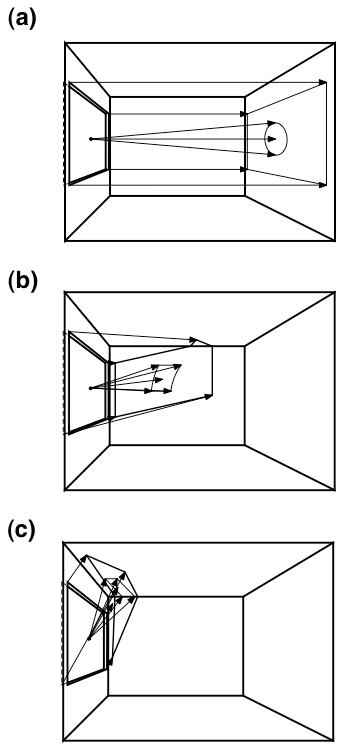
\includegraphics[width=0.9\textwidth, height=0.9\textheight, keepaspectratio=true]{media/image1326.png}
\caption{Transmitted Radiation in Three Directions for a Perimeter Office. (a) q = 0º; (b) q = 40º, f = 15º; (c) q = 70º, f = 67.5º.  q and f are the normal spherical angle coordinates in a right-handed coordinate system where y points up and z is normal to the window p \protect \label{fig:transmitted-radiation-in-three-directions-for}}
\end{figure}

\subparagraph{Complex Fenestrations in EnergyPlus}\label{complex-fenestrations-in-energyplus}

Exterior

EnergyPlus models the exterior radiance in two parts, a moving sun radiance \({S^{{\rm{(Sun)}}}}(t)\Delta {\Omega ^{{\rm{(Sun)}}}}\) ~and a constant-shape direction-dependent sky radiance \({S^{{\rm{(Sky)}}}}({\bf{p}},t)\) .~ The intensities of these vary with time.~ For the solar radiation there is a single sky radiance model.~ For daylight calculations the treatment is similar for exterior luminance, except that there are a number of user-selectable sky luminance models.~ Here we will discuss radiance; the treatment of luminance is analogous.

The direct normal solar intensity (at a given time) is

\begin{equation}
{I^{{\rm{(D)}}}}(t) = {S^{{\rm{(Sun)}}}}(t)\Delta {\Omega ^{{\rm{(Sun)}}}}
\end{equation}

and if we let

\begin{equation}
{S^{{\rm{(Sky)}}}}({\bf{p}},t) = {I^{{\rm{(Sky)}}}}(t)s({\bf{p}})
\end{equation}

where the shape function for the sky radiance model, \emph{s}, is defined so that

\begin{equation}
\int\limits_{2\pi } {s({\bf{p}})d\Omega }  = 1
\end{equation}

then the global solar irradiance on a horizontal surface at a given time is

\begin{equation}
{I^{{\rm{(G)}}}}(t) = {I^{{\rm{(Sky)}}}}(t)\left( {1 - \int\limits_{\Delta {\Omega ^{{\rm{(Sun)}}}}} {s({\bf{p}})d\Omega } } \right) + {I^{{\rm{(D)}}}}(t)\cos {\theta ^{{\rm{(Sun)}}}}(t)
\end{equation}

It must be understood that in equation the integration region 2p means integration over the sky hemisphere, and that \emph{s(\textbf{p})} is zero for upward-going directions.

With the sky radiance shape \emph{s(\textbf{p})} specified in the EnergyPlus code, the angular size of the sun \(\Delta {\Omega ^{{\rm{(Sun)}}}}\) ~known, and the solar zenith angle \({\theta ^{{\rm{(Sun)}}}}(t)\) ~calculated in the code, the two hourly input quantities \emph{I}\(^{(D*)*}\)\emph{(t)} and \emph{I}\(^{(G)}\)\emph{(t)} determine the exterior radiance for any given hour.

In this context, the transmitted radiance for a complex fenestration system given in equation becomes

\begin{equation}
\begin{array}{c}S({{\bf{p}}^{{\rm{(T)}}}}) = {I^{({\bf{Sky}})}}(t)\int\limits_{{\Omega ^{{\rm{(Sky)}}}}} {{\mathop{\rm T}\nolimits} ({{\bf{p}}^{{\rm{(T)}}}},{{\bf{p}}^{{\rm{(I)}}}})s({{\bf{p}}^{{\rm{(I)}}}})\left( { - {{\bf{p}}^{{\rm{(I)}}}}\cdot {\bf{n}}} \right)d{\Omega ^{{\rm{(I)}}}}} \\ + \int\limits_{{\Omega ^{{\rm{(Gnd)}}}}} {{\mathop{\rm T}\nolimits} ({{\bf{p}}^{{\rm{(T)}}}},{{\bf{p}}^{{\rm{(I)}}}}){S^{{\rm{(Gnd)}}}}({{\bf{p}}^{{\rm{(I)}}}},t)\left( { - {{\bf{p}}^{{\rm{(I)}}}}\cdot {\bf{n}}} \right)d{\Omega ^{{\rm{(I)}}}}} \\ + H\left( {\Delta {\Omega ^{{\rm{(Sun)}}}}(t) \not\subset {\Omega ^{{\rm{(Sf)}}}}} \right)\int\limits_{\Delta {\Omega ^{{\rm{(Sun)}}}}(t)} {{\mathop{\rm T}\nolimits} ({{\bf{p}}^{{\rm{(T)}}}},{{\bf{p}}^{{\rm{(I)}}}}){S^{{\rm{(Sun)}}}}({{\bf{p}}^{{\rm{(I)}}}},t)\left( { - {{\bf{p}}^{{\rm{(I)}}}}\cdot {\bf{n}}} \right)d{\Omega ^{{\rm{(I)}}}}} \\ + \int\limits_{{\Omega ^{{\rm{(Sf)}}}}} {{\mathop{\rm T}\nolimits} ({{\bf{p}}^{{\rm{(T)}}}},{{\bf{p}}^{{\rm{(I)}}}}){S^{{\rm{(Refl)}}}}({{\bf{p}}^{{\rm{(I)}}}},t)\left( { - {{\bf{p}}^{{\rm{(I)}}}}\cdot {\bf{n}}} \right)d{\Omega ^{{\rm{(I)}}}}} \end{array}
\end{equation}

where the incoming hemisphere viewed by the fenestration has been broken up into four parts.~ The viewed sky (excluding the part containing the sun) is \({\Omega ^{{\rm{(Sky)}}}}\) , the viewed ground is \({\Omega ^{{\rm{(Gnd)}}}}\) , the part subtended by the sun is DW\(^{(Sun)}\), and the part subtended by one or more exterior surfaces (shading or reflecting objects) is W\(^{(Sf)}\).~ These solid angles must exclude the exterior surfaces.~ The symbol \emph{H} represents a Helmholtz function: Its value is one if its logical argument is true, zero otherwise.~ It has been inserted into the equation to account for those times when the sun is behind an exterior object.~ Where there are multiple exterior shading or reflecting objects, W\(^{(Sf)}\) may consist of several regions that may be disjoint or connected, depending on the exterior geometry.~ As indicated in the equation, DW\(^{(Sun)}\) is time-dependent, to account for the sun's movement; W\(^{(Gnd)}\) and W\(^{(Sf)}\)~ are fixed, but as written \({\Omega ^{{\rm{(Sky)}}}}\) ~has a time dependence induced by the exclusion of the solid angle subtended by the sun.~ So that we can discuss the parts separately, we break the outgoing radiance down by source:

\begin{equation}
S({{\bf{p}}^{{\rm{(T)}}}}) = {S^{{\rm{(Sky)}}}}({{\bf{p}}^{{\rm{(T)}}}}) + {S^{{\rm{(Gnd)}}}}({{\bf{p}}^{{\rm{(T)}}}}) + {S^{{\rm{(Sun)}}}}({{\bf{p}}^{{\rm{(T)}}}}) + {S^{{\rm{(Sf)}}}}({{\bf{p}}^{{\rm{(T)}}}})
\end{equation}

By subtracting the radiation from the part of the sky hidden by the sun from \({S^{{\rm{(Sun)}}}}\) ~and adding it back into \emph{S}\(^{(Sky)}\) we can remove the time dependence of W\(^{(Sky)}\):

\begin{equation}
\begin{array}{c}{S^{{\rm{(Sun)}}}}({{\bf{p}}^{{\rm{(T)}}}}) = H\left( {\Delta {\Omega ^{{\rm{(Sun)}}}}(t) \not\subset {\Omega ^{{\rm{(Sf)}}}}} \right)\\ \times \int\limits_{\Delta {\Omega ^{{\rm{(Sun)}}}}(t)} {{\mathop{\rm T}\nolimits} ({{\bf{p}}^{{\rm{(T)}}}},{{\bf{p}}^{{\rm{(I)}}}})\left[ {{S^{{\rm{(Sun)}}}}({{\bf{p}}^{{\rm{(I)}}}},t) - {I^{({\bf{Sky}})}}(t)s({{\bf{p}}^{{\rm{(I)}}}})} \right]\left( { - {{\bf{p}}^{{\rm{(I)}}}}\cdot {\bf{n}}} \right)d{\Omega ^{{\rm{(I)}}}}} \end{array}
\end{equation}

\begin{equation}
{S^{{\rm{(Sky)}}}}({{\bf{p}}^{{\rm{(T)}}}}) = {I^{({\bf{Sky}})}}(t)\int\limits_{{\Omega ^{{\rm{(Sky)}}}}} {{\mathop{\rm T}\nolimits} ({{\bf{p}}^{{\rm{(T)}}}},{{\bf{p}}^{{\rm{(I)}}}})s({{\bf{p}}^{{\rm{(I)}}}})\left( { - {{\bf{p}}^{{\rm{(I)}}}}\cdot {\bf{n}}} \right)d{\Omega ^{{\rm{(I)}}}}}
\end{equation}

Now in equation the integral is to be evaluated without regard to the sun position, and therefore \({\Omega ^{{\rm{(Sky)}}}}\) ~is time-independent.

We can further simplify equation by noting that the angular size of the sun is small, and both \emph{s}(\textbf{\emph{p}}\(^{(I)}\)) and T(\textbf{\emph{p}}\(^{(T)}\), \textbf{\emph{p}}\(^{(I)}\)) can be considered as constant over the range of directions in DW\(^{(Sun)}\).~ We can therefore evaluate them at the direction \textbf{\emph{p}}\(^{(Sun)}\)(t) of the center of the sun and move them out of the integration, resulting in

\begin{equation}
{S^{{\rm{(Sun)}}}}({{\bf{p}}^{{\rm{(T)}}}}) = {\mathop{\rm T}\nolimits} ({{\bf{p}}^{{\rm{(T)}}}},{{\bf{p}}^{{\rm{(Sun)}}}})\left[ {{I^{{\rm{(D)}}}} - {I^{{\rm{(Sky)}}}}s({{\bf{p}}^{{\rm{(Sun)}}}})\Delta {\Omega ^{{\rm{(Sun)}}}}} \right]\cos {\theta ^{{\rm{(Sun)}}}}H\left( {{{\bf{p}}^{{\rm{(Sun)}}}} \not\subset {\Omega ^{{\rm{(Sf)}}}}} \right)
\end{equation}

In this equation we have dropped the explicit time dependence, but \textbf{\emph{p}}\(^{(Sun)}\), \emph{q}\(^{(Sun)}\), \emph{I}\(^{(D)}\), and \emph{I}\(^{(Sky)}\) are time-varying, while DW\(^{(Sun)}\) is simply the constant angular size of the sun.

We separate the reflected radiance \emph{S}\(^{(Sf)}\) into separate components for each surface,

\begin{equation}
{S^{{\rm{(Sf)}}}} = \sum\limits_n {{S^{{\rm{(Sf, n)}}}}}
\end{equation}

The individual shading surface reflected radiances are then

\begin{equation}
{S^{{\rm{(Sf, n)}}}}({{\bf{p}}^{{\rm{(T)}}}}) = \int\limits_{{\Omega ^{{\rm{(Sf, n)}}}}} {{\mathop{\rm T}\nolimits} ({{\bf{p}}^{{\rm{(T)}}}},{{\bf{p}}^{{\rm{(I)}}}}){S^{{\rm{(Refl, n)}}}}({{\bf{p}}^{{\rm{(I)}}}},t)\left( { - {{\bf{p}}^{{\rm{(I)}}}}\cdot {\bf{n}}} \right)d{\Omega ^{{\rm{(I)}}}}}
\end{equation}

The solid angle of integration in this expression is subtended by the portion of the exterior reflecting surface \emph{n} viewed by the fenestration; if one surface lies behind another, the hidden part of its surface is removed from the solid angle it subtends.~ This is summarized by the requirement

\begin{equation}
\begin{array}{l}{\Omega ^{{\rm{(Sf)}}}} = \bigcup\limits_n {{\Omega ^{{\rm{(Sf, n)}}}}} \\\bigcap\limits_n {{\Omega ^{{\rm{(Sf, n)}}}}}  = 0\end{array}
\end{equation}

(This requirement will need to be modified to handle the case of transmitting exterior surfaces.)

\emph{S}\(^{(Refl,n)}\) is time dependent because the incident radiation on the surface depends on the sun position. \emph{~}Equation must be evaluated after the exterior surface shading or reflectance calculations, in order to enforce the requirement that

\begin{equation}
{\Omega ^{{\rm{(Sky)}}}} \cap {\Omega ^{{\rm{(Sf)}}}} = 0
\end{equation}

Finally, the transmitted radiance from the ground-reflected exterior radiation is

\begin{equation}
{S^{{\rm{(Gnd)}}}}({{\bf{p}}^{{\rm{(T)}}}}) = \int\limits_{{\Omega ^{{\rm{(Gnd)}}}}} {{\mathop{\rm T}\nolimits} ({{\bf{p}}^{{\rm{(T)}}}},{{\bf{p}}^{{\rm{(I)}}}}){S^{{\rm{(Gnd)}}}}({{\bf{p}}^{{\rm{(I)}}}},t)\left( { - {{\bf{p}}^{{\rm{(I)}}}}\cdot {\bf{n}}} \right)d{\Omega ^{{\rm{(I)}}}}}
\end{equation}

Here, not only is there the requirement that

\begin{equation}
{\Omega ^{{\rm{(Gnd)}}}} \cap {\Omega ^{{\rm{(Sf)}}}} = 0
\end{equation}

but also the incident radiation on the ground may be affected by shading or reflection from exterior surfaces.~ Since this is dependent on the sun position, \emph{S}\(^{(Gnd)}\) is time dependent, as indicated in equation .

Applying the discretization of the previous section and the definitions in equations -, we can rewrite equation as

\begin{equation}
{S_j}^{{\rm{(T,Sky)}}} = {I^{({\bf{Sky}})}}(t)\sum\limits_{i \in {\Omega ^{{\rm{(Sky)}}}}} {{T_{ji}}{\Lambda_{ii}}{s_i}}
\end{equation}

where

\begin{equation}
{s_i} = s({{\bf{p}}_i}^{{\rm{(I)}}})
\end{equation}

is the sky radiance shape factor evaluated at the central direction of the i\(^{th}\) solid angle bin.~ A ``T'' superscript has been added on the left-hand side of the equation to denote that \emph{S} is the transmitted outgoing radiance (due to incident sky radiation for the fenestration under discussion).~ The stipulation \(i \in {\Omega ^{{\rm{(Sky)}}}}\) ~on the summation means that the sum is to include only those solid angle elements for which the sky is viewed by the fenestration.~ This is essentially a shading calculation, in addition to a restriction to downward-going incident directions.~ We anticipate the result of this calculation by defining a sky geometric factor:

\begin{equation}
V_i^{(Sky)} = \left\{
    \begin{array}{rl}
      1                      & \text{all of } \Delta\Omega_i \text{ views sky for all of fenestration} \\
      \text{viewed fraction} & \text{some of } \Delta\Omega_i \text{, fenestration views sky} \\
      0                      & \text{none of } \Delta\Omega_i \text{ views sky for any part of fenestration}
    \end{array}
  \right.
\end{equation}

Then we can carry out the summation over all downward directions and write

\begin{equation}
  S_j^{(T,Sky)} = I^{Sky}(t)\sum_{i down} T_{ji} \Lambda_{ii} V_i^{(Sky)} {s_i}
\end{equation}

Similarly, equation becomes

\begin{equation}
{S_j}^{{\rm{(T, Sf, n)}}} = \sum\limits_{i{\rm{ }}down} {{T_{ji}}{\Lambda_{ii}}V_i^{{\rm{(Sf, n)}}}{S^{{\rm{(Refl, n)}}}}({{\bf{p}}_i}^{{\rm{(I)}}},t)}
\end{equation}

where \(V_{i}^{(Sf,\, n)}\) is another geometric view factor, defined analogously to equation , giving the fraction of the solid angle \(\Delta {\Omega_i}\) that views the exterior surface \emph{n}. Note that

\begin{equation}
V_i^{{\rm{(Sky)}}} + \sum\limits_{\rm{n}} {V_i^{{\rm{(Sf, n)}}}}  = 1
\end{equation}

The quantity \(S^{(Refl,n)} (\bf{p}_i^{(I)},t)\) is in fact the reflected radiance at a particular location on the n\(^{th}\) exterior surface --- the location where the direction \textbf{\emph{p}}\emph{\(_{i}\)}\(^{(I)}\) intersects the surface. (This statement will become more precise when the spatial dependence dropped from equation is re-inserted.) This surface is assumed to have either a diffuse reflectance \emph{r}\(^{(n)}\) or a specular reflectance \emph{r}\(^{(sp,\\ n)}\). (Both properties are possible simultaneously, but EnergyPlus assumes that an exterior surface is either diffusing or specular, but not both.) The reflectance is assumed uniform over the surface, but the particular location (effectively, the image of the fenestration projected onto surface n) may or may not view the sky, or, at a particular time, the sun. We denote the incident irradiance of the surface n by \(E_i^n\). This irradiance pertains only to the surface n (in the present EnergyPlus calculation) and is independent of the fenestration or its basis.~ We attach the subscript i simply as a reminder that (2) the irradiance pertains to the portion of the surface that is viewed by the solid angle element \(\Delta {\Omega_i}\) of the fenestration f (which would become important if the EnergyPlus shading calculations were modified to relax the assumption of uniform incident irradiance on exterior surfaces) and that the irradiance pertains only to those surfaces n that are viewed by the solid angle element i. For specularly reflecting surfaces, we make the following definitions: First, within the set of basis solid angles \(\Delta {\Omega_i}\), let s(\emph{t}) identify the one containing the sun direction at time \emph{t}, and let r(\emph{t}) identify the one containing the specular reflection direction of the sun at time \emph{t}. We then define a contingent direct beam irradiance, which we denote by \(E_{i{\rm{ }}r(t)}^{(D,n)}\) . This irradiance is non-zero only if \(i = r(t)\) this direction is such that i is the specularly reflected direction for the surface n. If this is the case, then \(E_{i = r(t)}^{(D,n)}\) is the incident direct beam irradiance. With this definition,

\begin{equation}
{S^{{\rm{(Refl, n)}}}}({{\bf{p}}_i}^{{\rm{(I)}}},t) = {\rho ^{{\rm{(sp, n)}}}}E_{i{\rm{ }}r(t)}^{(D,n)} + {\rho ^{{\rm{(n)}}}}E_i^n
\end{equation}

If we then define normalized irradiance factors \emph{U} by \(E_i^n = U_i^{(Sky,n)}{I^{(Sky)}}(t) + U_{i{\rm{ }}Sun(tsh)}^{(D,n)}{I^{(D)}}(t)\) ~and \(E_{i{\rm{ }}r(t)}^{(D,n)} = U_{i{\rm{ }}r(t)}^{(D,n)}{I^{(D)}}(t)\) , where \(U_{i{\rm{ }}Sun(tsh)}^{(D,n)}\) ~denotes the fraction of the beam solar that irradiates the surface for a given sun direction.~ It is evaluated during the shading calculation, as indicated by the notation \emph{Sun(tsh)}.~ With these definitions we can rewrite the equation as

\begin{equation}
S^{(Refl,n)}(\bf{p}_i^{(I)},t) = 
  I^{(D)}(t) U_{i r(t)}^{(D,n)} \rho^{(sp,n)} +
  I^{(D)}(t) U_{i Sun(tsh)}^{(D,n)} \rho^{(n)} +
  I^{(sky)}(t) U_i^{(Sky,n)} \rho^{(n)}
\end{equation}

and equation becomes, in terms of the incident irradiances,

\begin{equation}
{S_j}^{{\rm{(T, Sf, n)}}} = \sum\limits_{i{\rm{ }}down} {{T_{ji}}{\Lambda_{ii}}V_i^{{\rm{(Sf, n)}}}\left( {{\rho ^{{\rm{(sp, n)}}}}E_{i{\rm{ }}r(t)}^{(D,n)} + {\rho ^{{\rm{(n)}}}}E_i^n} \right)}
\end{equation}

and in terms of the normalized irradiance factors,

\begin{equation}
\begin{array}{c}{S_j}^{{\rm{(T, Sf, n)}}} = \sum\limits_{i{\rm{ }}down} {{T_{ji}}{\Lambda_{ii}}V_i^{{\rm{(Sf, n)}}}{I^{{\rm{(D)}}}}(t)U_{i{\rm{ r(}}t{\rm{)}}}^{{\rm{(D,n)}}}{\rho ^{{\rm{(sp, n)}}}}} \\ + \sum\limits_{i{\rm{ }}down} {{T_{ji}}{\Lambda_{ii}}V_i^{{\rm{(Sf, n)}}}\left[ {{I^{{\rm{(D)}}}}(t)U_{i{\rm{ }}Sun(tsh)}^{{\rm{(D,n)}}}{\rho ^{{\rm{(n)}}}} + {I^{(Sky)}}(t)U_i^{{\rm{(Sky,n)}}}{\rho ^{{\rm{(n)}}}}} \right]} \end{array}
\end{equation}

The specularly reflected term can be removed from the sum, since only one value of i can contribute:

\begin{equation}
{S_j}^{{\rm{(T, Sf, n)}}} = {T_{j{\rm{ r(}}t{\rm{)}}}}{\Lambda_{{\rm{ r(}}t{\rm{) r(}}t{\rm{)}}}}V_{{\rm{ r(}}t{\rm{)}}}^{{\rm{(Sf, n)}}}E_{{\rm{ r(}}t{\rm{) r(}}t{\rm{)}}}^{{\rm{(D,n)}}}{\rho ^{{\rm{(sp, n)}}}} + {\rho ^{{\rm{(n)}}}}\sum\limits_{i{\rm{ }}down} {{T_{ji}}{\Lambda_{ii}}V_i^{{\rm{(Sf, n)}}}E_i^n}
\end{equation}

and

\begin{equation}
\begin{array}{c}{S_j}^{{\rm{(T, Sf, n)}}} = {T_{j{\rm{ r(}}t{\rm{)}}}}{\Lambda_{{\rm{ r(}}t{\rm{) r(}}t{\rm{)}}}}V_{{\rm{ r(}}t{\rm{)}}}^{{\rm{(Sf, n)}}}U_{{\rm{ r(}}t{\rm{) r(}}t{\rm{)}}}^{{\rm{(D,n)}}}{I^{(D)}}(t){\rho ^{{\rm{(sp, n)}}}}\\ + {\rho ^{{\rm{(n)}}}}\sum\limits_{i{\rm{ }}down} {{T_{ji}}{\Lambda_{ii}}V_i^{{\rm{(Sf, n)}}}\left( {{I^{{\rm{(D)}}}}(t)U_{i{\rm{ }}Sun(tsh)}^{{\rm{(D,n)}}} + U_i^{(Sky,n)}{I^{(Sky)}}(t)} \right)} \end{array}
\end{equation}

which separates specular and diffuse reflectance from the exterior surfaces.

With respect to shading and reflection of exterior radiation into the fenestration, the exterior reveal surfaces can be treated as additional diffusely reflecting exterior surfaces.

Ground radiation is treated in the same way as radiation reflected from interior surfaces, except that one sums only over upward-going incident directions, and the ground is assumed to be diffusely reflecting.~ The transmitted radiance from ground reflectance is

\begin{equation}
{S_j}^{{\rm{(T, Gnd)}}} = {\rho ^{{\rm{(Gnd)}}}}\sum\limits_{i{\rm{ }}up} {{T_{ji}}{\Lambda_{ii}}V_i^{{\rm{(Gnd)}}}E_i^{(Gnd)}}
\end{equation}

In this equation, the symbol \(E_i^{(Gnd)}\) ~is shorthand for a spatial calculation.~ The solid angle region \(\Delta {\Omega_i}\) ~views (from various points over the fenestration area) some spatial region of the ground.~ The symbol \(E_i^{(Gnd)}\) ~denotes the incident irradiance on the ground over this spatial region.~ In the absence of shading, this would be simply \({I^{(G)}} = {I^{(Sky)}} + {I^{(D)}}\cos {\theta_{Sun}}\) ; shading requires a more complex calculation.~ Currently the EnergyPlus code does a Monte-Carlo calculation: rays are randomly generated from the window, when they strike the ground a calculation is made to determine whether that point receives direct solar radiation and what portion of the sky it views (reflected radiation from surfaces is neglected).~ Here we would perform that calculation for each region of the ground i viewed by a basis solid angle element, instead of generating random rays from the window.~ We denote the results of that calculation by \(E_i^{(Gnd)} = U_{i{\rm{ }}Sun(tsh)}^{(D,Gnd)}{I^{(D)}}(t) + U_i^{(Sky,Gnd)}{I^{(Sky)}}(t)\) , where the \emph{U}'s are average viewing factors for the sun and sky, calculated as part of the shading calculation (which is indicated by the subscript \emph{tsh}: \emph{Sun(tsh)} is the sun direction as specified by the shading calculation.~ This then gives

\begin{equation}
{S_j}^{{\rm{(T, Gnd)}}} = {\rho ^{{\rm{(Gnd)}}}}\sum\limits_{i{\rm{ }}up} {{T_{ji}}{\Lambda_{ii}}V_i^{{\rm{(Gnd)}}}\left( {U_{i{\rm{ }}Sun(tsh)}^{(D,Gnd)}{I^{(D)}}(t) + U_i^{(Sky,Gnd)}{I^{(Sky)}}(t)} \right)}
\end{equation}

The transmitted radiance from direct beam radiation is

\begin{equation}
{S_j}^{{\rm{(T, Sun)}}} = {T_{j{\rm{ s}}(t)}}\cos {\theta ^{{\rm{(Sun)}}}}{I^{{\rm{(D)}}}}(t)V_{i{\rm{ s(}}t{\rm{)}}}^{{\rm{(D)}}}
\end{equation}

This introduces yet one more geometric view factor: $V_{i s(t)}^{(D)}$ is zero if the sun direction s\emph{(t)} is not \emph{i}; if \emph{i} = s(\emph{t}) it is the fraction of the fenestration area irradiated by the direct sun.~ Equation uses the fact that the angular size of the sun is smaller than any basis solid angle element, and that EnergyPlus treats the sun and circumsolar region as a point source {[}hence the absence of the sky correction in equation {]}.

At this point we have developed separate expressions for a fenestration's~ transmitted radiance in a particular direction depending on the exterior source of the radiation.~ These expressions utilize the discretized BTDF of the fenestration in the form of transmittance matrix elements over an angular basis.~ The exterior geometry is re-expressed in the form of geometric view factors in this basis.~ In the process, the explicit time dependence of the exterior radiation has been reduced to the time-varying direct and diffuse solar intensities and the solar position.~ The time dependence of the solar position, however, consists merely in specifying, for a particular time, which of the basis solid angle elements contains the solar direction.~ The entire exterior geometry necessary for the fenestration transmittance calculation can therefore be pre-calculated.

Interior

We begin with the discretized form of equation , in which we also modify the surface notation.~ In that equation, the surfaces involved are termed (1) and (2), where radiation is outgoing from surface 1 and incoming to surface 2.~ Here radiation is outgoing from the inner surface of the fenestration, so we label that surface (f).~ The receiving surface is one of the surfaces of the zone in which the fenestration is located.~ We number those surfaces with the index \emph{k}, so the receiving surface is labeled (\emph{k}).~ Equation then becomes

\begin{equation}
dW_j^{{\rm{(f}} \to k{\rm{)}}} = {E^{{\rm{(}}k{\rm{)}}}}({{\bf{p}}_j}^{{\rm{(T)}}})d{A^{{\rm{(}}k{\rm{)}}}} = {S_j}^{{\rm{(T)}}} \cdot \left( {{{\bf{n}}^{{\rm{(f)}}}} \cdot {{\bf{p}}_j}^{{\rm{(T)}}}} \right)\Delta {\Omega_j}^{{\rm{(T)}}}d{A^{{\rm{(f)}}}}
\end{equation}

or, noting that \(\left(\bf{n}^{(f)}\cdot\bf{p}_j^{(T)}\right) \Delta\Omega^{(T)} = \Lambda_{jj}^{(T)}\) ~(where the superscript T is retained in case the incoming and outgoing bases are defined differently),

\begin{equation}
dW_j^{{\rm{(f}} \to k{\rm{)}}} = {E^{{\rm{(}}k{\rm{)}}}}({{\bf{p}}_j}^{{\rm{(T)}}})d{A^{{\rm{(}}k{\rm{)}}}} = {S_j}^{{\rm{(T)}}}\Lambda_{jj}^{{\rm{(T)}}}d{A^{{\rm{(f)}}}}
\end{equation}

If we integrate this expression over the fenestration area \emph{A}\(^{(f)}\) we obtain the total power leaving the fenestration surface in direction \emph{j}; however, all of that power may not reach surface \emph{k}: some may strike the inner window reveal or a different zone surface.~ If we define a spatial projection operator by

\begin{equation}
{{\bf{x}}^{{\rm{(}}k{\rm{)}}}} = {{\mathop{\rm P}\nolimits} ^{{\rm{(}}k{\rm{)}}}}({\bf{p}}_j^{{\rm{(T)}}},{{\bf{x}}^{{\rm{(f)}}}}) \equiv {{\mathop{\rm P}\nolimits}_j}^{{\rm{(}}k{\rm{)}}}({{\bf{x}}^{{\rm{(f)}}}})
\end{equation}

where \textbf{\emph{x}}\(^{(*k*)}\) is in the plane of surface \emph{k}, and a geometric form factor by

\begin{equation}
F_j^{{\rm{(}}k{\rm{)}}} = \frac{1}{{{A^{{\rm{(f)}}}}}}\int\limits_{{{\mathop{\rm P}\nolimits}_j}^{{\rm{(}}k{\rm{)}}}({{\bf{x}}^{{\rm{(f)}}}}) \in {A^{{\rm{(}}k{\rm{)}}}}} {d{A^{{\rm{(f)}}}}}
\end{equation}

then

\begin{equation}
dW_j^{{\rm{(f}} \to k{\rm{)}}} = {S_j}^{{\rm{(T)}}}\Lambda_{jj}^{{\rm{(T)}}}F_j^{{\rm{(}}k{\rm{)}}}{A^{{\rm{(f)}}}}
\end{equation}

The total power leaving the fenestration (in any direction) and arriving at surface \emph{k} is then

\begin{equation}
W_j^{{\rm{(f}} \to k{\rm{)}}} = \sum\limits_j {{S_j}^{{\rm{(T)}}}\Lambda_{jj}^{{\rm{(T)}}}F_j^{{\rm{(}}k{\rm{)}}}{A^{{\rm{(f)}}}}}
\end{equation}

Substituting equations , , , , into equation yields a series of expressions for the total power arriving at surface \emph{k} (by transmission through fenestration f) from each of the sources of exterior radiation.~ However, the equations for transmitted radiation describe an infinitesimal region, which means that the radiation in a given direction will always come from one source.~ When one integrates the transmitted power over the fenestration surface, one encounters the problem that for this direction different parts of the fenestration area may receive radiation from different sources.~ Also, for a given outgoing direction, the projection of a receiving surface back onto the fenestration may produce an image that covers only part of the fenestration area, and this image may not be identical with the part of the area that receives incident radiation from a particular source.~ The most important origin of this problem is the existence of inner and outer window reveals, as illustrated in Figure~\ref{fig:mismatch-of-irradiated-and-viewed}.

\begin{figure}[hbtp] % fig 93
\centering
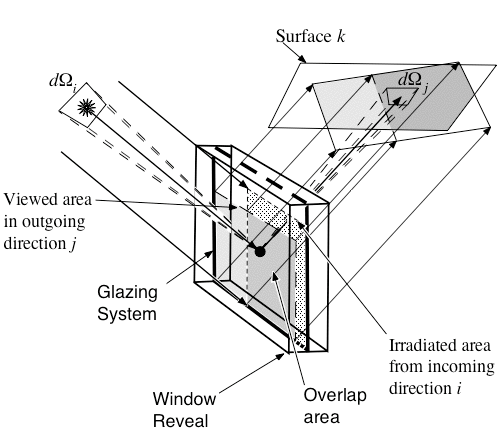
\includegraphics[width=0.9\textwidth, height=0.9\textheight, keepaspectratio=true]{media/image1392.png}
\caption{Mismatch of irradiated and viewed fenestration areas for different incident and outgoing directions \protect \label{fig:mismatch-of-irradiated-and-viewed}}
\end{figure}

In this figure, the portion of the fenestration area not viewed by the plane of surface \emph{k} is instead viewed by one or more of the inner window reveals.~ Similarly, the portion of the fenestration not irradiated in the figure is in fact irradiated by diffusely reflected radiation from the outer window reveals.~ We can account for this by replacing the area \emph{A}\(^{(f)}\) in equation with the overlap area \(A_{ji}^{{\rm{(f, Src), }}k}\) \emph{~}(dark shaded in the figure), where ``Src'' stands for the source of the incident radiation.~ This area is defined by

\begin{equation}
A_{ji}^{\left( {f,Src} \right),k} = \left. {A_i^{\left( {f,Src} \right)}} \right|A_j^{\left( f \right),k}
\end{equation}

The total power at the interior surface \emph{k} for each source of radiation then becomes

\begin{equation}
{W^{{\rm{(Sky), }}k}} = {I^{({\bf{Sky}})}}(t)\sum\limits_j {\Lambda_{jj}^{{\rm{(T)}}}F_j^{{\rm{(}}k{\rm{)}}}\sum\limits_{i{\rm{ }}down} {{T_{ji}}{\Lambda_{ii}}V_i^{{\rm{(Sky)}}}A_{ji}^{{\rm{(f, Sky), }}k}{s_i}} }
\end{equation}

\begin{equation}
\begin{array}{c}{W^{{\rm{(Sf,n)}},k}} = {I^{{\rm{(D)}}}}(t){\rho ^{{\rm{(sp, n)}}}}\sum\limits_j {\Lambda_{jj}^{{\rm{(T)}}}F_j^{{\rm{(}}k{\rm{)}}}{T_{j{\rm{ r(}}t{\rm{)}}}}{\Lambda_{{\rm{ r(}}t{\rm{) r(}}t{\rm{)}}}}V_{{\rm{ r(}}t{\rm{)}}}^{{\rm{(Sf, n)}}}A_{j{\rm{ r(}}t{\rm{)}}}^{{\rm{(f, Sf, n), }}k}U_{{\rm{ r(}}t{\rm{) s(}}t{\rm{)}}}^{{\rm{(D,n)}}}} \\ + {I^{(D)}}(t){\rho ^{{\rm{(n)}}}}\sum\limits_j {\Lambda_{jj}^{{\rm{(T)}}}F_j^{{\rm{(}}k{\rm{)}}}\sum\limits_{i{\rm{ }}down} {{T_{ji}}{\Lambda_{ii}}V_i^{{\rm{(Sf, n)}}}A_{ji}^{{\rm{(f, Sf, n), }}k}U_{i{\rm{ }}Sun(tsh)}^{{\rm{(D,n)}}}} } \\ + {I^{(Sky)}}(t){\rho ^{{\rm{(n)}}}}\sum\limits_j {\Lambda_{jj}^{{\rm{(T)}}}F_j^{{\rm{(}}k{\rm{)}}}\sum\limits_{i{\rm{ }}down} {{T_{ji}}{\Lambda_{ii}}V_i^{{\rm{(Sf, n)}}}A_{ji}^{{\rm{(f, Sf, n), }}k}U_i^{{\rm{(Sky,n)}}}} } \end{array}
\end{equation}

\begin{equation}
\begin{array}{c}{W^{{\rm{(Gnd)}},k}} = {I^{{\rm{(D)}}}}(t){\rho ^{{\rm{(Gnd)}}}}\sum\limits_j {\Lambda_{jj}^{{\rm{(T)}}}F_j^{{\rm{(}}k{\rm{)}}}\sum\limits_{i{\rm{ }}up} {{T_{ji}}{\Lambda_{ii}}V_i^{{\rm{(Gnd)}}}A_{ji}^{{\rm{(f, Gnd), }}k}U_{i{\rm{ }}Sky(tch)}^{{\rm{(D, Gnd)}}}} } \\ + {I^{({\bf{Sky}})}}(t){\rho ^{{\rm{(Gnd)}}}}\sum\limits_j {\Lambda_{jj}^{{\rm{(T)}}}F_j^{{\rm{(}}k{\rm{)}}}\sum\limits_{i{\rm{ }}up} {{T_{ji}}{\Lambda_{ii}}V_i^{{\rm{(Gnd)}}}A_{ji}^{{\rm{(f, Gnd), }}k}U_i^{{\rm{( Sky,Gnd)}}}} } \end{array}
\end{equation}

\begin{equation}
{W^{{\rm{(Sun)}},k}} = {I^{{\rm{(D)}}}}(t)\sum\limits_j {F_j^{{\rm{(}}k{\rm{)}}}\Lambda_{jj}^{{\rm{(T)}}}{T_{j{\rm{ s}}(t)}}\cos {\theta_{{\rm{s(}}t{\rm{)}}}}^{{\rm{(Sun)}}}V_{i{\rm{ s(}}t{\rm{)}}}^{{\rm{(D)}}}A_{j{\rm{ s(}}t{\rm{)}}}^{{\rm{(f, Sun), }}k}}
\end{equation}

If we define a series of solar irradiation factors, Z, that describe the fraction of the radiation incident on the fenestration due to a given exterior radiation source that is ultimately incident on the interior surface \emph{k},

\begin{equation}
{Z^{{\rm{(Sky), }}k}} = \sum\limits_j {\Lambda_{jj}^{{\rm{(T)}}}F_j^{{\rm{(}}k{\rm{)}}}\sum\limits_{i{\rm{ }}down} {{T_{ji}}{\Lambda_{ii}}V_i^{{\rm{(Sky)}}}A_{ji}^{{\rm{(f, Sky), }}k}{s_i}} }
\end{equation}

\begin{equation}
{Z_{{\rm{r(}}t{\rm{)}}}}^{{\rm{(sp, Sf, n)}},k} = \sum\limits_j {\Lambda_{jj}^{{\rm{(T)}}}F_j^{{\rm{(}}k{\rm{)}}}{T_{j{\rm{ r(}}t{\rm{)}}}}{\Lambda_{{\rm{ r(}}t{\rm{) r(}}t{\rm{)}}}}V_{{\rm{ r(}}t{\rm{)}}}^{{\rm{(Sf, n)}}}A_{j{\rm{ r(}}t{\rm{)}}}^{{\rm{(f, Sf, n), }}k}U_{{\rm{ r(}}t{\rm{) s(}}t{\rm{)}}}^{{\rm{(D,n)}}}}
\end{equation}

\begin{equation}
{Z_{{\rm{s(}}t{\rm{)}}}}^{{\rm{(Sun, Sf, n)}},k} = \sum\limits_j {\Lambda_{jj}^{{\rm{(T)}}}F_j^{{\rm{(}}k{\rm{)}}}\sum\limits_{i{\rm{ }}down} {{T_{ji}}{\Lambda_{ii}}V_i^{{\rm{(Sf, n)}}}A_{ji}^{{\rm{(f, Sf, n), }}k}U_{i{\rm{ }}Sun(tsh)}^{{\rm{(D,n)}}}} }
\end{equation}

\begin{equation}
{Z^{{\rm{(Sky, Sf, n)}},k}} = \sum\limits_j {\Lambda_{jj}^{{\rm{(T)}}}F_j^{{\rm{(}}k{\rm{)}}}\sum\limits_{i{\rm{ }}down} {{T_{ji}}{\Lambda_{ii}}V_i^{{\rm{(Sf, n)}}}A_{ji}^{{\rm{(f, Sf, n), }}k}U_i^{{\rm{(Sky, n)}}}} }
\end{equation}

\begin{equation}
{Z_{{\rm{s(}}t{\rm{)}}}}^{{\rm{(D, Gnd)}},k} = \sum\limits_j {\Lambda_{jj}^{{\rm{(T)}}}F_j^{{\rm{(}}k{\rm{)}}}\sum\limits_{i{\rm{ }}up} {{T_{ji}}{\Lambda_{ii}}V_i^{{\rm{(Gnd)}}}A_{ji}^{{\rm{(f, Gnd), }}k}U_{i{\rm{ }}Sun(tsh)}^{{\rm{(D, Gnd)}}}} }
\end{equation}

\begin{equation}
{Z^{{\rm{(Sky, Gnd)}},k}} = \sum\limits_j {\Lambda_{jj}^{{\rm{(T)}}}F_j^{{\rm{(}}k{\rm{)}}}\sum\limits_{i{\rm{ }}up} {{T_{ji}}{\Lambda_{ii}}V_i^{{\rm{(Gnd)}}}A_{ji}^{{\rm{(f, Gnd), }}k}U_i^{{\rm{(Sky, Gnd)}}}} }
\end{equation}

\begin{equation}
{Z_{{\rm{s(}}t{\rm{)}}}}^{{\rm{(Sun)}},k} = \sum\limits_j {F_j^{{\rm{(}}k{\rm{)}}}\Lambda_{jj}^{{\rm{(T)}}}{T_{j{\rm{ s}}(t)}}\cos {\theta_{{\rm{s(}}t{\rm{)}}}}^{{\rm{(Sun)}}}V_{i{\rm{ s(}}t{\rm{)}}}^{{\rm{(D)}}}A_{j{\rm{ s(}}t{\rm{)}}}^{{\rm{(f, Sun), }}k}}
\end{equation}

then equations through become

\begin{equation}
{W^{{\rm{(Sky), }}k}} = {I^{({\bf{Sky}})}}(t){Z^{{\rm{(Sky), }}k}}
\end{equation}

\begin{equation}
\begin{array}{c}{W^{{\rm{(Sf,n)}},k}} = {I^{{\rm{(D)}}}}(t){\rho ^{{\rm{(sp, n)}}}}{Z_{{\rm{r(}}t{\rm{)}}}}^{{\rm{(sp, Sf, n)}},k} + {I^{{\rm{(D)}}}}(t){\rho ^{{\rm{(n)}}}}{Z_{{\rm{s(}}t{\rm{)}}}}^{{\rm{(Sun, Sf, n)}},k}\\ + {I^{({\bf{Sky}})}}(t){\rho ^{{\rm{(n)}}}}{Z^{{\rm{(Sky, Sf, n)}},k}}\end{array}
\end{equation}

\begin{equation}
{W^{{\rm{(Gnd)}},k}} = {I^{{\rm{(D)}}}}(t){\rho ^{{\rm{(Gnd)}}}}{Z_{{\rm{s(}}t{\rm{)}}}}^{{\rm{(D, Gnd)}},k} + {I^{({\bf{Sky}})}}(t){\rho ^{{\rm{(Gnd)}}}}{Z^{{\rm{(Sky, Gnd)}},k}}
\end{equation}

\begin{equation}
{W^{{\rm{(Sun)}},k}} = {I^{{\rm{(D)}}}}(t){Z_{{\rm{s(}}t{\rm{)}}}}^{{\rm{(Sun)}},k}
\end{equation}

The notation s(\emph{t}) appearing in a subscript in several of the above equations refers to the basis direction for which the sun direction is contained in the basis solid angle element.~ This is of course time dependent.~ What is meant here is that at any given time the particular basis element containing the sun is to be picked out.~ (If no basis element for the fenestration contains the sun at a given time, then the corresponding view factor---and therefore irradiance or absorption factor---is zero.)~ It is therefore necessary to tabulate those quantities with an s(\emph{t}) subscript for all basis directions \emph{s} that could possibly contain the sun direction (and for \emph{r(t)}, all basis directions that could possibly contain the reflected sun angle for the surface n).~ This is a set considerably smaller than that of all incoming basis directions.~ Figure~\ref{fig:sun-paths-and-incident-basis-for-three-window} illustrates this point for direct irradiation of fenestrations in three different orientations in a building at a particular latitude, using the W6 full basis, which has 145 incoming directions.~ In the worst case (west-facing) one only needs to consider around 50 of these, with much fewer needed in other orientations.~ The specific numbers for a given fenestration will depend on the choice of basis, orientation and latitude.~ The basis direction values can of course be interpolated where greater directional resolution is warranted.~ In equation the specular direction r(\emph{t}) is uniquely determined by the sun direction s(\emph{t}), so the Z factor does not need an additional index for \emph{s}.

\begin{figure}[hbtp] % fig 94
\centering
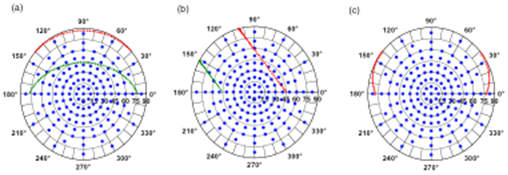
\includegraphics[width=0.9\textwidth, height=0.9\textheight, keepaspectratio=true]{media/image1410.png}
\caption{Sun Paths and Incident Basis for Three Window Orientations, 38º N. Latitude. The nodal positions (blue dots) for a W6 full basis are compared with the summer solstice (red curve) and winter solstice (green curve) solar paths. Solar paths for other days of the year will lie between these two extremes. (Note: the basis points are to be interpreted as the direction of a vector pointing from the fenestration to the sun.) (a) South facing. (b) West facing. (c) North facing (the winter path is off the figure (i.e., the window is shaded); allowed paths will be outside the red path. \protect \label{fig:sun-paths-and-incident-basis-for-three-window}}
\end{figure}

The reason for the definition of the Z factors is that to a great extent they can be precalculated, so that within the hourly calculation only equations - need to be used.~ In addition, there are fewer Z factors to be stored than transmittance matrix elements.~ The storage determinants for the foregoing calculations are summarized in the following table.

% table 35
\begin{longtable}[c]{p{1.5in}p{4.5in}}

\caption{Determination of array sizes \label{table:determination-of-array-sizes}} \tabularnewline
\toprule
\multicolumn{2}{c}{Parameters} \tabularnewline
\midrule
\endfirsthead

\caption[]{Determination of array sizes} \tabularnewline
\toprule
\multicolumn{2}{c}{Parameters} \tabularnewline
\midrule
\endhead

N\(_{Basis}\) & Number of elements in the (incoming or outgoing) basis \tabularnewline
N\(_{Sun}\) & Number of basis directions that may be sun directions (depends on fenestration orientation \tabularnewline
N\(^{(Gnd)}_{Sun}\) & Number of sun directions that give significantly different ground irradiation conditions, as seen by fenestration \tabularnewline
N\(_{Sf}\) & Number of reflecting surfaces viewable by fenestration (depends on fenestration orientation) \tabularnewline
N\(^{(Sf,n)}_{Sun}\) & Number of time steps for which surface \emph{n} is sunlit (depends on orientation of surface \emph{n}; determined during shading calculation) \tabularnewline
N\(^{(Sf,n)}_{Refl}\) & Number of basis directions that may be reflected sun directions from surface \emph{n} (depends on orientation of fenestration and surface \emph{n}). \tabularnewline
N\(_{IntSurf}\) & Number of interior surfaces in the zone containing the fenestration \tabularnewline
N\(_{Layers}\) & Number of thermal layers in the fenestration system \tabularnewline
\multicolumn{2}{c}{Arrays} \tabularnewline
A\(^{F,l}_{i}\), A\(^{B,l}_{i}\) & Absorptance vector element; N\(_{Basis}\) \tabularnewline
T\(_{ij}\) & Transmittance matrix element; N\(_{Basis}\) X N\(_{Basis}\) \tabularnewline
V\(^{(Sky)}_{i}\) & Sky viewed fraction; one-dimensional, N\(_{Basis}\) \tabularnewline
V\(^{(Sf,n)}_{i}\) & Fraction of surface \emph{n} viewed; N\(_{Basis}\) X N\(_{Sf}\) \tabularnewline
$\rho$\(^{(n)}\), $\rho$\(^{(sp,n)}\) & Surface \emph{n} diffuse, specular reflectance; N\(_{Sf}\) (already stored by E+) \tabularnewline
U\(^{(D,n)}_{i\,Sun(tsh)}\) & Fraction of the image of $\Delta\Omega$\(_{i}\) on surface \emph{n} that views the sun when it is in direction Sun(tsh); N\(_{Basis}\) X N\(_{Sf}\) X N\(^{(Sf,n)}_{Sun}\) \tabularnewline
V\(^{(Gnd)}_{i}\) & Fraction of $\Delta\Omega$\(_{i}\) that views ground; N\(_{Basis}\) \tabularnewline
U\(^{(Sky, Gnd)}_{i}\) & Fraction of sky radiation received by the image of $\Delta\Omega$\(_{i}\) on the ground; N\(_{Basis}\) \tabularnewline
U\(^{(D,Gnd)}_{i\,Sun(tsh)}\) & Fraction of direct solar radiation for sun direction Sun(tsh) received by image of $\Delta\Omega$\(_{i}\) on ground; N\(^{Gnd}_{Sim}\) X N\(_{Basis}\) \tabularnewline
V\(^{(D)}_{i\,s(t)}\) & Fraction of fenestration area irradiated by direct solar radiation for direction \emph{i}, given that sun angle is s(\emph{t}); N\(_{Sun}\) X N\(_{Basis}\) \tabularnewline
F\(^{(k)}_{j}\) & Fraction of radiation in direction \emph{j} leaving fenestration interior that arrives at surface \emph{k}; N\(_{Basis}\) X N\(_{IntSurf}\) \tabularnewline
Z\(^{(Sky), k}\) & Sky irradiation factor; N\(_{IntSurf}\) \tabularnewline
Z\(^{(sp,Sf,n),k}_{r(t)}\) & Exterior surface specular irradiation factor; N\(^{(Sf,n)}_{Sun}\) X N\(_{Sf}\) X N\(_{IntSurf}\) \tabularnewline
Z\(^{(Sun,Sf,n),k}_{s(t)}\) & Exterior surface direct-diffuse irradiation factor; N\(^{(Sf,n)}_{Sun}\) X N\(_{Sf}\) X N\(_{IntSurf}\) \tabularnewline
Z\(^{(Sky,Sf,n),k}\) & Exterior surface sky irradiation factor; N\(_{Sf}\) X N\(_{IntSurf}\) \tabularnewline
Z\(^{(D,Gnd),k}_{s(t)}\) & Ground-reflected direct solar irradiaton factor (given sun direction s(\emph{t})); N\(^{(Gnd)}_{Sun}\) X N\(_{IntSurf}\) \tabularnewline
Z\(^{(Sky,Gnd),k}\) & Ground-reflected diffuse solar irradiation factor; N\(_{IntSurf}\) \tabularnewline
Z\(^{(Sun),k}_{s(t)}\) & Direct solar irradiation factor; N\(_{Sun}\) X N\(_{IntSurf}\) \tabularnewline
K\(^{(Sky),l}\) & Sky absorption factor; N\(_{Layers}\) \tabularnewline
K\(^{(sp,Sf,n),l}_{r(t)}\) & Exterior surface specular absorption factor; N\(_{Sf}\) X N\(^{(Sf,n)}_{Refl}\) X N\(_{Layers}\) \tabularnewline
K\(^{(Sun,Sf,n),l}_{s(t)}\) & Exterior surface diffusely reflected direct sun absorption factor; N\(_{Sf}\) X N\(^{(Sf,n)}_{Sun}\) X N\(_{Layers}\) \tabularnewline
K\(^{(Sky,Sf,n),l}\) & Exterior surface reflected sky radiation absorption factor; N\(_{Sf}\) X N\(_{Layers}\) \tabularnewline
K\(^{(D,Gnd),l}_{s(t)}\) & Ground-reflected direct solar absorption factor; N\(^{(Gnd)}_{Sun}\) X N\(_{Layers}\) \tabularnewline
K\(^{(Sky,Gnd),l}\) & Ground-reflected sky radiation absorption factor; N\(_{Layers}\) \tabularnewline
K\(^{(Sun),l}_{s(t)}\) & Direct sunlight absorption factor; N\(_{Sun}\) X N\(_{Layers}\) \tabularnewline
\bottomrule
\end{longtable}

\subparagraph{Absorption}\label{absorption}

For thermal calculations it is necessary to know the energy absorbed in each layer of the fenestration.~ This depends only on the incident geometry, but otherwise is calculated in the same manner as the solar flux incident on interior surfaces. ~For a given layer l of a fenestration f, we define a source-referenced absorption factor, K(source),l.~ This is the amount of energy absorbed in layer l divided by the relevant solar intensity (which might be beam, diffuse, or reflected beam or diffuse, depending on the source of the radiation).~ These absorption factors and the resultant source-specific absorbed solar powers are calculated by the analogs {[}see equation of equations through :

\begin{equation}
{K^{{\rm{(Sky), }}l}} = {A^{{\rm{(f)}}}}\sum\limits_{i{\rm{ }}down} {{\mathop{\rm A}\nolimits}_i^{F,l}{\Lambda_{ii}}V_i^{{\rm{(Sky)}}}{s_i}}
\end{equation}

\begin{equation}
{Q^{{\rm{(Sky), }}l}} = {I^{({\bf{Sky}})}}(t){K^{{\rm{(Sky), }}l}}
\end{equation}

\begin{equation}
{K_{{\rm{r(}}t{\rm{)}}}}^{{\rm{(sp, Sf, n)}},l} = {A^{{\rm{(f)}}}}{\mathop{\rm A}\nolimits}_{r(t)}^{F,l}{\Lambda_{{\rm{ r(}}t{\rm{) r(}}t{\rm{)}}}}V_{{\rm{ r(}}t{\rm{)}}}^{{\rm{(Sf, n)}}}U_{{\rm{ r(}}t{\rm{) s(}}t{\rm{)}}}^{{\rm{(D,n)}}}
\end{equation}

\begin{equation}
{K_{{\rm{s(}}t{\rm{)}}}}^{{\rm{(Sun, Sf, n)}},l} = {A^{{\rm{(f)}}}}\sum\limits_{i{\rm{ }}down} {{\mathop{\rm A}\nolimits}_i^{F,l}{\Lambda_{ii}}V_i^{{\rm{(Sf, n)}}}U_{i{\rm{ }}Sun(tsh)}^{{\rm{(D,n)}}}}
\end{equation}

\begin{equation}
{K^{{\rm{(Sky, Sf, n)}},l}} = {A^{{\rm{(f)}}}}\sum\limits_{i{\rm{ }}down} {{\mathop{\rm A}\nolimits}_i^{F,l}{\Lambda_{ii}}V_i^{{\rm{(Sf, n)}}}U_i^{{\rm{(Sky, n)}}}}
\end{equation}

\begin{equation}
\begin{array}{c}{Q^{{\rm{(Sf,n)}},l}} = {I^{{\rm{(D)}}}}(t){\rho ^{{\rm{(sp, n)}}}}{K_{{\rm{r(}}t{\rm{)}}}}^{{\rm{(sp, Sf, n)}},l} + {I^{{\rm{(D)}}}}(t){\rho ^{{\rm{(n)}}}}{K_{{\rm{s(}}t{\rm{)}}}}^{{\rm{(Sun, Sf, n)}},l}\\ + {I^{({\bf{Sky}})}}(t){\rho ^{{\rm{(n)}}}}{K^{{\rm{(Sky, Sf, n)}},l}}\end{array}
\end{equation}

\begin{equation}
{K_{{\rm{s(}}t{\rm{)}}}}^{{\rm{(D, Gnd)}},l} = {A^{{\rm{(f)}}}}\sum\limits_{i{\rm{ }}up} {{\mathop{\rm A}\nolimits}_i^{F,l}{\Lambda_{ii}}V_i^{{\rm{(Gnd)}}}U_{i{\rm{ }}Sun(tsh)}^{{\rm{(D, Gnd)}}}}
\end{equation}

\begin{equation}
{K^{{\rm{(Sky, Gnd)}},l}} = {A^{{\rm{(f)}}}}\sum\limits_{i{\rm{ }}up} {{\mathop{\rm A}\nolimits}_i^{F,l}{\Lambda_{ii}}V_i^{{\rm{(Gnd)}}}U_i^{{\rm{(Sky, Gnd)}}}}
\end{equation}

\begin{equation}
{Q^{{\rm{(Gnd)}},l}} = {I^{{\rm{(D)}}}}(t){\rho ^{{\rm{(Gnd)}}}}{K_{{\rm{s(}}t{\rm{)}}}}^{{\rm{(D, Gnd)}},l} + {I^{({\bf{Sky}})}}(t){\rho ^{{\rm{(Gnd)}}}}{K^{{\rm{(Sky, Gnd)}},l}}
\end{equation}

\begin{equation}
{K_{{\rm{s(}}t{\rm{)}}}}^{{\rm{(Sun)}},l} = {A^{{\rm{(f)}}}}{\mathop{\rm A}\nolimits}_{{\rm{s}}(t)}^{F,l}\cos {\theta_{{\rm{s(}}t{\rm{)}}}}^{{\rm{(Sun)}}}V_{i{\rm{ s(}}t{\rm{)}}}^{{\rm{(D)}}}
\end{equation}

\begin{equation}
{Q^{{\rm{(Sun)}},l}} = {I^{{\rm{(D)}}}}(t){K_{{\rm{s(}}t{\rm{)}}}}^{{\rm{(Sun)}},l}
\end{equation}

\subparagraph{Comment on Bases}\label{comment-on-bases}

Use of the basis in the above discussion has been mostly implicit, but it should nevertheless be clear that the essential feature of the basis is that it is a two-element list (i.e., a 2 X N array): it associates with an incident (i) or outgoing (j) direction index a vector pi (or pj ) that is a unit vector giving the direction of the radiation, the specification of which is two angles in some coordinate system.~ The incident and outgoing bases of course must match the matrix elements of the fenestration properties.~ These bases will (certainly in the case of WINDOW program; probably in the case of other input sources) have a structure: ordering of the elements, etc.~ However, after the initialization of the hourly loop calculation, this structure will be irrelevant:~ EnergyPlus will retain only those incoming and outgoing directions that are essential to the calculation with (one would hope, most of) the others combined into irradiation factors.~ At this point, the basis will truly be an arbitrary list.~ It follows that the specification of the basis in the EnergyPlus input should be determined by (1) the source of fenestration property data, and (2) user convenience.

A related point concerns the specification of a basis for specular glazings, i.e., multiple layers of glass.~ These fenestrations are both specular (input direction = output direction) and axially symmetric.~ These properties have different effects on the calculation.

The specular property means that one should not be using equation at all to describe the transmittance.~ Instead, one should use the equation

\begin{equation}
S({{\bf{p}}^{{\rm{(T)}}}}) = \tau ({{\bf{p}}^{{\rm{(T)}}}}) \cdot E({{\bf{p}}^{{\rm{(T)}}}})
\end{equation}

This equation is shoehorned into the integral calculation of equation through the use of a delta function in the incident direction vector, resulting (after the discretization) in a diagonal matrix for the transmittance (or reflectance).~ The outgoing radiance element on the diagonal would be calculated as \emph{T\(_{ii}\)}L\emph{\(_{ii}\)}, where multiplication by L\emph{\(_{ii}\)} substitutes for integration over the basis solid angle element. For a specular glazing, \(T_{ii} = \tau(\bf{p}_i^{(T)})/\Lambda_{ii}\), so one recovers the correct transmittance when one does the multiplication. However, there is still a problem in principle: For a specular fenestration, the angular spread of the outgoing radiation will be that of the source, which for direct sunlight is very small; the calculation, however, assumes the angular spread of the basis element. This problem disappears in the geometric approximation to be used in EnergyPlus: by considering only the central direction of each basis element, the outgoing radiation in that direction is essentially assumed to be specular, so the blurring in the discretization is undone.

The axial symmetry of conventional glazings means that the transmittance (or reflectance) depends on only the incident angle, not the azimuthal angle about the normal to the fenestration plane.~ So if one specifies the diagonal elements of the matrix, all of the terms with the same incident angles but different azimuthal angles will be the same.~ One could alternatively specify only the specular transmittance at each of the incident angle values, provided one also indicated that it was for an axially symmetric fenestration.~ Since expanding this set of values to the equivalent diagonal elements is a trivial calculation, how one specifies a specular glazing is completely a question of user convenience.~ For example, if one were dealing with the WINDOW full basis, would it be more user-friendly to specify

\begin{enumerate}
\def\labelenumi{(\arabic{enumi})}
\item
  \(T_{ii} = \tau(\bf{p}_i^{(T)})/\Lambda_{ii}\) , for 145 values, 135 of which are repeats of the previous value
\item
  \(\tau ({\theta_i})\) ~for 9 values of incident angle, \emph{q\(_{i}\)} ?
\end{enumerate}

\subparagraph{Interior Solar Radiation Transmitted by Complex Fenestration}\label{interior-solar-radiation-transmitted-by-complex-fenestration}

Diffuse Solar Radiation Transmitted by Complex Fenestration

Distribution of solar radiation transmitted through exterior window is divided on diffuse and direct part.

Diffuse solar transmitted through exterior complex fenestration and absorbed in interor walls is calculated and treated in same way as described in the section on Initial Distribution of Diffuse Solar Transmitted through Exterior and Interior Windows. Even though that BSDF is given for various directions, for purpose of diffuse solar radiation, transmittance and reflectances of fenestration system is integrated over incoming and outgoing hemisphere.~ Because incoming diffuse solar radiation is divided on ground and sky parts, integration of incoming hemisphere is also perfomed over ground and sky part (see equation .

Direct Solar Radiation Transmitted by Complex Fenestration

Direct solar (beam) transmitted through exterior window is using same overlap calculations (see Figure~\ref{fig:vertical-section-through-a-two-zone-building}) for each outgoing basis direction.~ For certain sun position, algorithm calculatates equivalent incoming beam number.~ The inside beam solar irradiance is calculated in similar manner as described in the section titled Interior Beam Radiation.

\begin{equation}
\begin{split}
AISurf\left(SurfNum\right) =& \frac{AbsIntSurf\left(SurfNum\right)}{A\left(SurfNum\right)} \\
&\cdot\sum_{i = 1}^{N_{extwin}} \left( \sum_{j = 1}^{N_{out}} TB{m_{k,j}} \cdot \Lambda_{k,j} \cdot \text{Aoverlap}_{k,j} \left( SurfNum \right)\right) \cdot \text{CosInc}_i
\end{split}
\end{equation}

\emph{i} = exterior window number

\emph{N\(_{extwin}\) =} number of exterior windows in zone

\emph{N\(_{out}\) =} Beam number of exterior windows in zone

\emph{CosInc\(_{i}\)} = cosine of angle of incidence of beam on exterior window \emph{i}

\emph{TBm\(_{k,j}\)} = beam-to-beam transmittance of exterior window* i*at incidence direction k outgoing direction j

\emph{Λ\(_{k,j}\)} = lambda value of exterior window* i*at incidence direction k for outgoing direction j

\emph{Aoverlap\(_{k,j}\)(SurfNum)} = beam solar irradiated area of surface \emph{SurfNum} projected back onto the plane of exterior window* i* for incoming direction k and outgoing direction j (the \emph{Aoverlap}'s for an exterior window sum up to the glazed area of the window)

\emph{AbsIntSurf(SurfNum)} = inside face solar absorptance of surface \emph{SurfNum}

\emph{A(SurfNum)} = area of surface \emph{SurfNum} {[}m\(^{2}\){]}

Equation is valid as long as surface which is hit by transmitted solar radiation is not another complex fenestration.~ In that case, for beam which is transmitted from other exterior window and reaches back surface of this window, angle of incidence needs to be taken into account.

\subparagraph{Interior Solar Absorbed by Complex Fenestration}\label{interior-solar-absorbed-by-complex-fenestration}

Solar radiation absorbed in window layers is coming from three sources: Diffuse radiation from sky and ground, direct radiation from the sun and beam radiation coming from the sun and it is transmitted through other exterior windows.

Diffuse Radiation from Sky and Ground

Energy absorbed in the layers and which originates from diffuse radiation from sky and ground is represented by following equation:

\begin{equation}
\begin{split}
&\text{QRadSWwinAbs}(Surf, Lay) = \\
&\sum_{i = 1}^{N_{layers}} \left(\text{WinSkyFtAbs}(Surf, Lay) \cdot \text{SkySolarInc} + \text{WinSkyGndAbs}(Surf, Lay) \cdot \text{GndSolarInc}\right)
\end{split}
\end{equation}

where,

\emph{WinSkyFtAbs(Lay)} = front absorptance averaged over sky for layer (Lay) and window belonging to Surf

\emph{WinSkyGndAbs(Lay)} = front absorptance averaged over ground for layer (Lay) and window belonging to Surf

\emph{SkySolarInc =} incident diffuse solar from the sky

\emph{GndSolarInc} = incident diffuse solar from the ground

Direct Radiation from the Sun

Energy absorbed in the layers and which originates from direct solar radiation is given by following equation:

\begin{equation}
\text{QRadSWwinAbs}(SurfNum, Lay) = \text{AWinSurf}(SurfNum, Lay) \cdot \text{BeamSolar}
\end{equation}

where,

\emph{AWinSurf(SurfNum,Lay)} -- is time step value of factor for beam absorbed in fenestration glass layers

\emph{BeamSolar} -- Current beam normal solar irradiance

Factor for time step value is given by equation:

\begin{equation}
\begin{split}
\text{AWinSurf}(SurfNum,Lay) =& \text{WinBmFtAbs}(Lay,HourOfDay,TimeStep) \cdot \text{CosInc} \\
&\cdot \text{SunLitFract} \cdot \text{OutProjSLFracMult}(HourOfDay)
\end{split}
\end{equation}

where,

\emph{WinBmFtAbs(Lay,HourOfDay,TimeStep)} -- is front directional absorptance for given layer and time

\emph{CosInc} -- cosine of beam solar incident angle

\emph{SunLitFract} -- sunlit fraction without shadowing effects of frame and divider

\emph{OutProjSLFracMult(HourOfDay)} - Multiplier on sunlit fraction due to shadowing of glass by frame and divider outside projections.

Direct Solar Radiation Coming from Sun and it is Transmitted Through Other Windows

Direct solar radiation transmitted through other windows is using solar overlap calculations described in the section on Overlapping Shadows. Overlapping is used to determine amount of energy transferred through the window is hitting certain surface.~ That is used to calculate energy absorbed in walls and same approach will be used to calculate energy absorbed in window layers (equation ).~ In case when receiving surface is complex fenestration, it is not enought just to apply equation because factor AbsIntSurf is now depending of incoming angle which is defined through front and back directional absorptance matrices.~ It would mean that for each outgoing directions of transmitting complex fenestration, algorithm would need to determine what is best matching basis direction of receiving surface.~ Best receiving direction is used to determine absorptance factors which will be used in equation .~ It is important to understand that for basis definition, each unit vector defining one beam is going towards surface, which would mean that best matching directions from surface to surface will actually have minimal dot product.

\begin{equation}
Bes{t_{in}} = {\rm{min}}\left( {dot\left( {ou{t_p},i{n_1}} \right),dot\left( {ou{t_p},i{n_2}} \right), \ldots ,dot\left( {ou{t_p},i{n_N}} \right)} \right)
\end{equation}

where,

Best\(_{in}\) -- is best matching receiving direction basis dot product (in\(_{k}\))

out\(_{p}\) -- current transmitting complex fenestration direction

in\(_{1}\), \ldots{}, in\(_{N}\) -- set of receiving complex fenestration basis directions

Result of equation is minimal dot product, which corresponds to best matching direction of receiving surface.~ If we mark that direction with index k, then equation becomes:

\begin{equation}
  \begin{array}{l}
    AWinSurf(SurfNum,Lay) = \\
      \frac{1}{A(SurfNum)} \cdot \\
      \sum_{i = 1}^{N_{extwin}} (\sum\limits_{j = 1}^{N_{out}} AbsIntSur{f_k}(SurfNum) \cdot TB{m_{k,j}} \cdot \\
      A_{k,j} \cdot \text{Aoverlap}_{k,j}(SurfNum)) \cdot \text{CosInc}_i
  \end{array}
\end{equation}

where,

\emph{AbsIntSurf\(_{k}\)(SurfNum)} -- directional absorptance for the receiving surface for the best matching direction

Everything else is same as described in equation .

\subsubsection{References}\label{references-1-018}

Klems, J. H. 1994A. ``A New Method for Predicting the Solar Heat Gain of Complex Fenestration Systems: I. Overview and Derivation of the Matrix Layer Calculation.''. ASHRAE Transactions. 100(pt.1): 1073-1086.

Klems, J. H. 1994B. ``A New Method for Predicting the Solar Heat Gain of Complex Fenestration Systems: II. Detailed Description of the Matrix Layer Calculation.''. ASHRAE Transactions. 100(pt.1): 1073-1086.

Klems, J. H. 1995. ``Measurements of Bidirectional Optical Properties of Complex Shading Devices.''. ASHRAE Transactions. 101(pt 1; Symposium Paper CH-95-8-1(RP-548)): 791-801.

Klems, J. H. 1996. ``A Comparison between Calculated and Measured SHGC for Complex Glazing Systems.''. ASHRAE Transactions. 102(Pt. 1; Symposium Paper AT-96-16-1): 931-939.

Klems, J. H. 1996. ``Calorimetric Measurements of Inward-Flowing Fraction for Complex Glazing and Shading Systems.''. ASHRAE Transactions. 102(Pt. 1; Symposium Paper AT-96-16-3): 947-954.

Papamichael, K. J. 1998. ``Determination and Application of Bidirectional Solar-Optical Properties of Fenestration Systems.''. Cambridge, MA: 13th National Passive Solar Conference.
